\documentclass[ms,cpyr,lof,lot]{uathesis}





\usepackage{graphicx}
\usepackage{amsmath,amssymb}
\usepackage{xcolor}
\usepackage{mathtools}
\usepackage{etoolbox}
\usepackage{booktabs}
\usepackage{float}
\usepackage{graphicx}
\usepackage{geometry}
\usepackage{multicol}
\usepackage{caption}
\usepackage{natbib}
\usepackage{siunitx}
\usepackage{listings}
\usepackage{bm}
\usepackage[outdir=./eps2pdf/]{epstopdf}
\graphicspath{
  {figures/}
  {figures/goals/}
  {figures/light_data/}
  {figures/attenuation/}
  {figures/results/}
}


\setlength{\tabcolsep}{12pt}

\definecolor{commentcolor}{HTML}{752000}
\definecolor{keywordcolor}{HTML}{007520}

\lstset{
    language=[90]Fortran,
    inputpath=../kelp/code/fortran/src,
    basicstyle=\linespread{0.8}\ttfamily,
    commentstyle=\rmfamily,
    keywordstyle=\color{commentcolor},
    commentstyle=\color{keywordcolor},
    showstringspaces=false,
    numbers=left,
    breaklines=true,
    numbersep=1em,
    frame=leftline,
    tabsize=4,
    xleftmargin=.5in,
    xrightmargin=.5in}

\DeclareMathOperator{\atantwo}{atan2}

\newcommand\xmin{{x_{\min}}}
\newcommand\xmax{{x_{\max}}}
\newcommand\ymin{{y_{\min}}}
\newcommand\ymax{{y_{\max}}}
\newcommand\zmin{{z_{\min}}}
\newcommand\zmax{{z_{\max}}}

\newcommand\plotwidth{7in}


\newcommand{\ds}{\displaystyle}

\newcommand{\erf}{\mbox{erf}}
\newcommand{\sign}{\mbox{sign}}
\newcommand{\ceil}{\mbox{ceil}}
\newcommand{\floor}{\mbox{floor}}
\newcommand\R{\mathbb{R}}
\newcommand\norm[1]{||#1||}
\newcommand\LL{\mathcal{L}}
\newcommand\FF{\mathcal{F}}


\newcommand\NN{\mathbb{N}}
\newcommand\RR{\mathbb{R}}
\newcommand\CC{\mathbb{C}}
\newcommand\BB{\mathcal{B}}
\newcommand\DD{\mathcal{D}}
\newcommand\QQ{\mathcal{Q}}
\newcommand\unorm[1]{\left\lVert #1 \right\rVert_\infty}
\newcommand\ip[1]{\left\langle #1 \right\rangle}
\newcommand\abs[1]{\left| #1 \right|}
\newcommand\conj\overline
\newcommand\pd[2]{\frac{\partial #1}{\partial #2}}
\newcommand{\iter}[1]{^{(#1)}}
\newcommand\qed{\hfill$\blacksquare$\hspace{0.5in}}

\renewcommand\vec\bm

\newcommand\nomega{{n_{\vec{\omega}}}}


\title{Modelling the Light Field in Macroalgae Aquaculture}
\author{Oliver Graham Evans}
\conferraldate{May}{2018}

\advisor{Dr. Kevin Kreider}
\chair{Dr. Kevin Kreider}
\collegedean{Dr. John Green}
\gradschdean{Dr. Chand Midha}
\coadvisor{Dr. Curtis Clemons}
\facreader{Dr. Gerald Young}

\begin{document}

\maketitle
\chapter{INTRODUCTION} \label{ch:intro}

\section{Motivation}
  Given the global rise in population, efficient and innovative resource utilization is increasingly important.
Future generations face major challenges regarding food, energy, and water security while addressing major issues associated with global climate change.
Growing concern for the negative environmental impacts of petroleum-based fuel is generating a market for biofuel, especially corn-based ethanol.
However, corn-based ethanol has been heavily criticized for diverting land usage away from food production, for increasing use of fertilizers that impair water quality, and for low return on energy investments for production.
At the same time, a great deal of unutilized saltwater coastline is available for both food and fuel production through seaweed cultivation.
Specifically, the sugar kelp \textit{Saccharina latissima} is known to be a viable source of food,  both for direct human consumption and biofuel production.

Nitrogen leakage into water bodies is a significant ecological problem, and is especially relevant near large conventional agriculture facilities due to run-off from nitrogen-based fertilizers, as well as near wastewater treatment plants.
Waste water treatment plants (WWTPs) in particular are facing increasingly stringent regulation of nutrients in their effluent discharges from the US Environmental Protection Agency (USEPA) and state regulatory agencies.
Nutrient management at WWTPs requires significant infrastructure, operations, and maintenance investments for tertiary treatment processes. Many treatment works are constrained financially or by space limitations in their ability to expand their treatment works.
As an alternative to conventional nutrient remediation techniques, the cultivation of the macroalgae \textit{Saccharina latissima} (sugar kelp) within the nutrient plume of WWTP ocean outfalls has been proposed.
The purpose of such an undertaking would be twofold: to prevent eutrophication of the surrounding ecosystem by sequestering nutrients, and to provide supplemental nutrients that benefit macroalgae cultivation. 

Large scale macroalgae cultivation has long existed in Eastern Asia due to the popularity of seaweed in Asian cuisine, and low labor costs that facilitate its manual seeding and harvest.
  More recently, less labor-intense and more industrialized kelp aquaculture has been developing in Scandinavia and in the Northeastern United States and Canada.
For example, the MACROSEA project is a four year international research collaboration led by SINTEF, an independent research organization in Norway, and funded by the Research Council of Norway targeting ``successful and predictable production of high quality biomass thereby making significant steps towards industrial macroalgae cultivation in Norway.'' 
The project includes both cultivators and scientists, working to develop a precise understanding of the full life cycle of kelp and its interaction with its environment.
A fundamental aspect of this endeavor is the development of mathematical models to describe the growth of kelp.

Recently, a growth model\cite{broch_modelling_2012} for S. latissima has been produced and integrated into the SINMOD\cite{wassmann_modelling_2006} hydrodynamic and ecosystem model of SINTEF.
One aspect of the model which has yet to be fully developed is the availability of light, considering factors such as absorption and scattering by the aquatic medium, as well as by the kelp itself.
This thesis contributes to this effort by developing a first-principles model of the light field in a kelp farming environment.
As a first step, a model for the spatial distribution of kelp is developed.
Radiative transfer theory is then applied to determine the effects of the kelp and water on the availability of light throughout the medium.
A finite difference solution to the radiative transfer equation is developed, followed by asymptotic approximations that prove to be sufficiently accurate for clear water, and significantly less computationally intensive.
A detailed description of the numerical solution of this model is presented, accompanied by source code for a FORTRAN implementation of the solution.
This model can be used independently, or in conjunction with a kelp growth model to determine the amount of light available for photosynthesis at a single time step.

\begin{figure}[h]
  \centering
  \includegraphics[width=0.5\textwidth]{kelp_photo/sonja}
  \caption{\textit{Saccharina latissima} being harvested}
\end{figure}


\section{Background on Kelp Models}

Mathematical modeling of macroalgae growth is not a new topic, although it is a reemerging one.
Several authors in the second half of the twentieth century were interested in describing the growth and composition of the macroalgae \textit{Macrocystis pyrifera}, commonly known as ``giant kelp,'' which grows prolifically off the coast of southern California.
The first such mathematical model was developed by W.J. North for the Kelp Habitat Improvement Project at the California Institute of Technology in 1968 using seven variables.
By 1974, Nick Anderson greatly expanded on North's work, and created the first comprehensive model of kelp growth which he programmed using FORTRAN\cite{anderson_mathematical_1974}.
In his model, he accounts for solar radiation intensity as a function of time of year and time of day, and refraction on the surface of the water.
He uses a simple model for shading, simply specifying a single parameter which determines the percentage of light that is allowed to pass through the kelp canopy floating on the surface of the water.
He also accounts for attenuation due to turbidity using Beer's Law.
Using this data on the availability of light, he calculates the photosynthesis rates and the growth experienced by the kelp.

Over a decade later in 1987, G.A.
Jackson expanded on Anderson's model for \textit{Macrocystis pyrifera}, with an emphasis on including more environmental parameters and a more complete description of the growth and decay of the kelp\cite{jackson_modelling_1987}. 
The author takes into account respiration, frond decay, and sub-canopy light attenuation due to self-shading.
Light attenuation is represented with a simple exponential model, and self-shading appears as an added term in the decay coefficient.
The author does not consider radial or angular dependence on shading. 
Jackson also expands Anderson's definition of canopy shading, treating the canopy not as a single layer, but as 0, 1, or 2 discrete layers, each composed of individual fronds.
While this is a significant improvement over Anderson's light model, it is still rather simplistic.

Both Anderson's and Jackson's model were carried out by numerically solving a system of differential equations over small time intervals.
In 1990, M.A. Burgman and V.A. Gerard developed a stochastic population model\cite{burgman_stage-structured_1990}.
This approach is quite different, and functions by dividing kelp plants into groups based on size and age and generating random numbers to determine how the population distribution over these groups changes over time based on measured rates of growth, death, decay, light availability, etc.
In the same year, Nyman et. al. published a similar model alongside a Markov chain model, and compared the results with experimental data collected in New Zealand\cite{nyman_macrocystis_1990}.

In 1996 and 1998 respectively, P. Duarte and J.G. Ferreira used the size-class approach to create a more general model of macroalgae growth, and Yoshimori et. al. created a differential equation model of \textit{Laminaria religiosa} with specific emphasis on temperature dependence of growth rate\cite{duarte_model_1997,yoshimori_mathematical_1998}.
These were the some of the first models of kelp growth that did not specifically relate to \textit{Macrocystis pyrifera} (``giant kelp''). 
Initially, there was a great deal of excitement about this species due to it's incredible size and growth rate, but difficulties in harvesting and negative environmental impacts have caused scientists to investigate other kelp species. 

\section{Background on Radiative Transfer}
In terms of optical quantities, of primary interest is in the radiance at each point from all directions, which affects the photosynthetic rate of the kelp, and therefore the total amount of biomass producible in a given area as well as the total nutrient remediation potential.
The equation governing the radiance throughout the system is known as the radiative transfer equation (RTE), which has been largely unutilized in the fields of oceanography and aquaculture.
The radiative transfer equation has been used primarily in stellar astrophysics; it's application to marine biology is fairly recent\cite{mobley_radiative_2001}.
In its full form, radiance is a function of 3 spatial dimensions, 2 angular dimensions, and frequency, making for an incredibly complex problem. 
In this work, frequency is ignored, only monochromatic radiation is considered.
The RTE states that along a given path, radiance is decreased by absorption and scattering out of the path, while it is increased by emission and scattering into the path.
In our situation, emission is negligible, owing only perhaps to some small luminescent phytoplankton or other anomaly, and can therefore be safely ignored.

Understanding the growth rate and nutrient recovery by
kelp cultures has important marine biological implications. For example, recent
work by our research group at Clarkson University, the University of Maine, and
SINTEF Fisheries and Aquaculture is investigating kelp aquaculture as a means to
recover nutrients from wastewater effluent plumes in coastal environments into a
valuable biomass feedstock for many products. Current models for kelp growth
place little emphasis on the way in which nearby plants shade one another.
Self-shading may be a significant model feature, though, as light availability
may impact the growth and composition of the kelp biomass, and thus the mixture
of goods that may be derived.

\section{Overview of Thesis}
The remainder of this document is organized as follows.
In Chapter \ref{chap:kelp}, probabilistic model is developed to describe the spatial distribution of kelp by assuming simple distributions for the lengths and orientations of fronds.
Chapter \ref{chap:light} begins with a survey of fundamental radiometric quantities and optical properties of matter.
The spatial kelp distribution from Chapter \ref{chap:kelp} is used to determine optical properties of the combined water-kelp medium,
and the radiative transfer equation, an integro-partial differential equation which describes the the light field as a function of position and angle, is discussed.
An asymptotic expansion is explored for cases where absorption dominates scattering in the medium, such as in very clear water or high kelp density.
In Chapter \ref{chap:numerical}, details are given for the numerical solution of the equations from Chapters \ref{chap:kelp} and \ref{chap:light}.
Both the full finite difference solution and the asymptotic approximation are described.
Next, in Chapter \ref{chap:parameters}, the availability of necessary parameters in the literature is discussed.
For those which are not readily available, give rough estimates are given or describe experimental methods for their determination are described.
Then, in Chapter \ref{chap:model_analysis}, necessary grid resolution for adequate accuracy in the full finite difference solution is determined.
The finite difference solution is compared to the asymptotic approximation for a few sets of optical properties.
Further, we showcase the effect of varying a few key parameters on the light field predicted by the asymptotic approximation.
Afterwards, the light model developed here is used in a numerical simulation of kelp growth, and the predicted light field and biomass production are compared to those predicted by a simpler 1D exponential decay light model.
Finally, Chapter \ref{chap:conclusion} concludes the thesis by giving a brief summary of the model, discuss and its performance, and suggest improvements and avenues for future work.
 \chapter{KELP MODEL}
\label{chap:kelp}

In order to properly model the spatial distribution of light around the kelp, it is first necessary to formulate a spatial description of the kelp, which we do in this chapter.
We take a probabilistic approach to describing the kelp.
We begin by describing the distribution of kelp fronds, and through algebraic manipulation, we are able to assign to each point in space a probability that kelp occupies the location.

\section{Physical Setup}
The life of cultivated macroalgae generally begins in the laboratory, where microscopic kelp spores are inoculated onto a thread in a small laboratory pool. 
This thread is wrapped around a large rope, which is placed in the ocean and generally suspended by buoys in one of two configurations: horizontal or vertical.
We consider only the case of a rigid vertical rope which does not sway in the current.
The mature \textit{Saccharina latissima} plant consists of a single frond (leaf), a stipe (stem) and a holdfast (root structure).
For the sake of this model, only the kelp frond is considered, and its base is attached directly to the rope.
The ``gentle undulation approximation'' is employed, whereby it is assumed that fronds are perfectly horizontal.
While on at any point in time they may point up or down due to water current and gravity, we consider the horizontal
state to be an average configuration.
This simplifaction allows for the three-dimensionally distributed population of kelp fronds
to be considered a collection of independent populations in two-dimensional depth layers.

\begin{figure}[H]
	\centering
	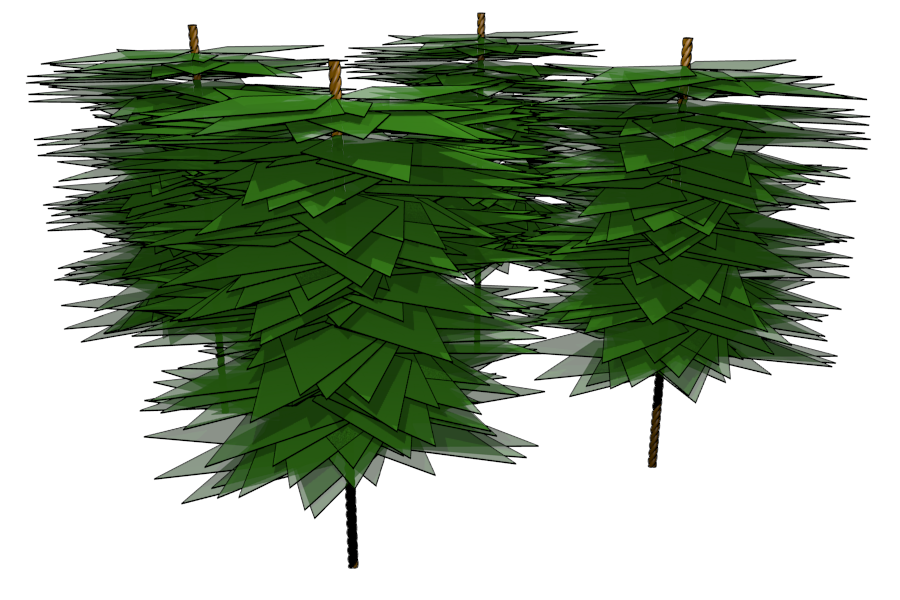
\includegraphics[width=3.5in]{kelp_array}
	\captionof{figure}{Rendering of four nearby vertical kelp ropes}
\end{figure}

\section{Coordinate System}
Consider the rectangular domain
\begin{align*}
  \xmin &\leq x \leq \xmax, \\
  \ymin &\leq y \leq \ymax, \\
  \zmin &\leq z \leq \zmax.
\end{align*}
For all three dimensional analysis, we use the absolute coordinate system defined in Figure \ref{fig:3dcoords}.
In the following sections, it is necessary to convert between Cartesian and spherical coordinates, which we do using the relations
\begin{equation}
  \left\{
	\begin{split}
		x & = r\sin\phi\cos\theta, \\
		y & = r\sin\phi\sin\theta, \\
		z & = r\cos\phi. \\
	\end{split}
  \right.
	\label{eqn:coords}
\end{equation}

Therefore, for some function $f(x,y,z)$, we can write its derivative along a path in spherical coordinates in terms of Cartesian coordinates using the chain rule.
\begin{equation*}
	\frac{\partial f}{\partial r} 
	=\frac{\partial f}{\partial x}\frac{\partial x}{\partial r} 
	+ \frac{\partial f}{\partial y}\frac{\partial y}{\partial r} 
	+ \frac{\partial f}{\partial z}\frac{\partial z}{\partial r}
\end{equation*}
Then, calculating derivatives from \eqref{eqn:coords} yields
\begin{equation}
	\frac{\partial f}{\partial r} 
	=\frac{\partial f}{\partial x}\sin\phi\cos\theta
	+ \frac{\partial f}{\partial y}\sin\phi\sin\theta
	+ \frac{\partial f}{\partial z}\cos\phi.
	\label{eqn:partials}
\end{equation}
\begin{figure}[H]
	\centering
	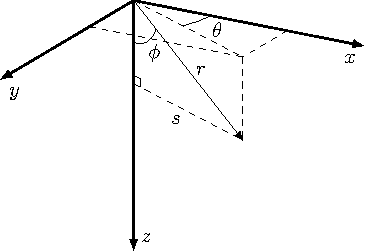
\includegraphics[width=3in]{3d_coords}
	\caption{Downward-facing right-handed coordinate system with radial distance $r$ from the origin, distance $s$ from the $z$ axis, zenith angle $\phi$ and azimuthal angle $\theta$}
	\label{fig:3dcoords}
\end{figure}


\section{Population Distributions}
In order to construct a spatial distribution of kelp fronds, a simple kite-shaped geometry is introduced,
and frond lengths and azimuthal orientations are assumed to be distributed predictably.
It is assumed that fronds extend perfectly horizontally 

\subsection{Frond Shape}
\label{sec:shape}

\begin{figure}[h]
	\centering
  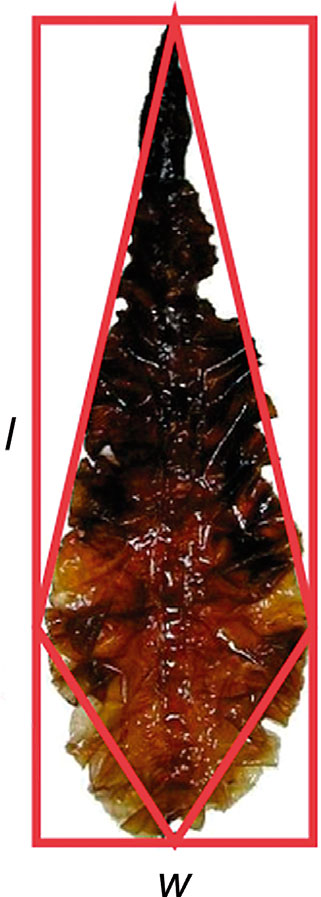
\includegraphics[width=1.2in]{kelp_photo/kite}
  \qquad
	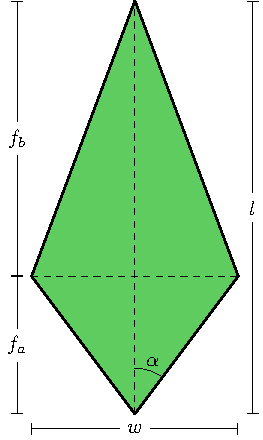
\includegraphics[width=2in]{frond}
	\captionof{figure}{Simplified kite-shaped frond}
	\label{fig:frond}
\end{figure}

The frond is assumed to be kite-shaped with length $l$ from base to tip, and width $w$ from left to right.
In Figure \ref{fig:frond}, the base is shown at the bottom and the tip is shown at the top.
The proximal length is the shortest distance from the base to the diagonal connecting the left and right corners, and is notated as $f_a$.
Likewise, the distal length is the shortest distance from that diagonal to the tip, notated $f_b$.
 We have
 \begin{equation*}
	 f_a + f_b = l
 \end{equation*}
When considering a whole population with varying sizes, it is more convenient to specify ratios than absolute lengths.
Let the following ratios be defined.
\begin{align*}
	f_r &= \frac{l}{w} \\
	f_s &= \frac{f_a}{f_b}
\end{align*}
These ratios are assumed to be consistent among the entire population, making all fronds geometrically similar.
With these definitions, the shape of the frond can be fully specified by $l$, $f_r$, and $f_s$.
It is possible, then, to redefine $w$, $f_a$ and $f_b$ as follows from the preceding formulas.

\begin{align*}
	w &= \frac{l}{f_r} \\
	f_a &= \frac{lf_s}{1+f_s} \\
	f_b &= \frac{l}{1+f_s}
\end{align*}

The angle $\alpha$, half of the angle at the base corner, is also noteworthy.
Using the above equations,
\begin{equation*}
	\alpha = \tan^{-1}\left(\frac{2f_rf_s}{1+f_s}\right)
\end{equation*}

The area of the frond is given by
\begin{equation*}
  A = \frac{lw}{2} = \frac{l^2}{2f_r}.
\end{equation*}

Likewise, if the area is known, then the length is
\begin{equation}
  l = \sqrt{2Af_r}.
  \label{eqn:length-from-area}
\end{equation}

\subsection{Length and Angle Distributions}
\label{sec:dist}
Frond lengths are assumed to be normally distributed with mean $\mu_l$ and standard deviation $\sigma_l$.
That is, the frond length distribution has the probability density function (PDF)
\begin{equation*}
  P_l(l) = \frac{1}{\sqrt{2\pi\sigma_l^2}}\exp\left(\frac{(l-\mu_l)^2}{2\sigma_l^2}\right).
\end{equation*}

It is further assumed that frond angle varies according to the von Mises distribution, which is the periodic analogue of the normal distribution, defined on $[-\pi,\pi]$ rather than $(-\infty,\infty)$.
The von Mises distribution has two parameters, $\mu$ and $\kappa$, which shift and sharpen its peak respectively, as shown in Figure \ref{fig:vonmises}.
$\kappa$ can be considered analogous to $1/\sigma$ in the normal distribution.
That is, in the case of zero current velocity, the frond angles are be distributed uniformly, while as current velocity increases, they become increasingly likely to be pointing in the direction of the current, depending on the stiffness of the frond.
Assuming a linear relationship between the current velocity and the steepness of the angular distribution, define the frond bending coefficient $\eta$, with units \SI{}{\s\per\m}.
Then, in use $\mu = \theta_w$ and $\kappa = \eta v_w$ as the von Mises distribution parameters.
Note that $\theta_w$ and $v_w$ vary over depth, while $\eta$ is assumed constant for the population.
Then, the PDF for the von Mises frond angle distribution is
\begin{equation*}
	P_{\theta_f}(\theta_f) = \frac{\exp\left(\eta v_w\cos(\theta_f-\theta_w)\right)}{2\pi I_0(\eta v_w)},
\end{equation*}
where $I_0(x)$ is the modified Bessel function of the first kind of order 0.
Notice that unlike the normal distribution, the von Mises distribution approaches a \textit{non-zero} uniform distribution as $\kappa$ approaches 0, so
\begin{equation*}
	\displaystyle \lim_{v_w \to 0}P_{\theta_f}(\theta_f) = \frac{1}{2\pi} \;\forall\, \theta_f \in [-\pi,\pi].
\end{equation*}

\begin{figure}[h]
	\centering
	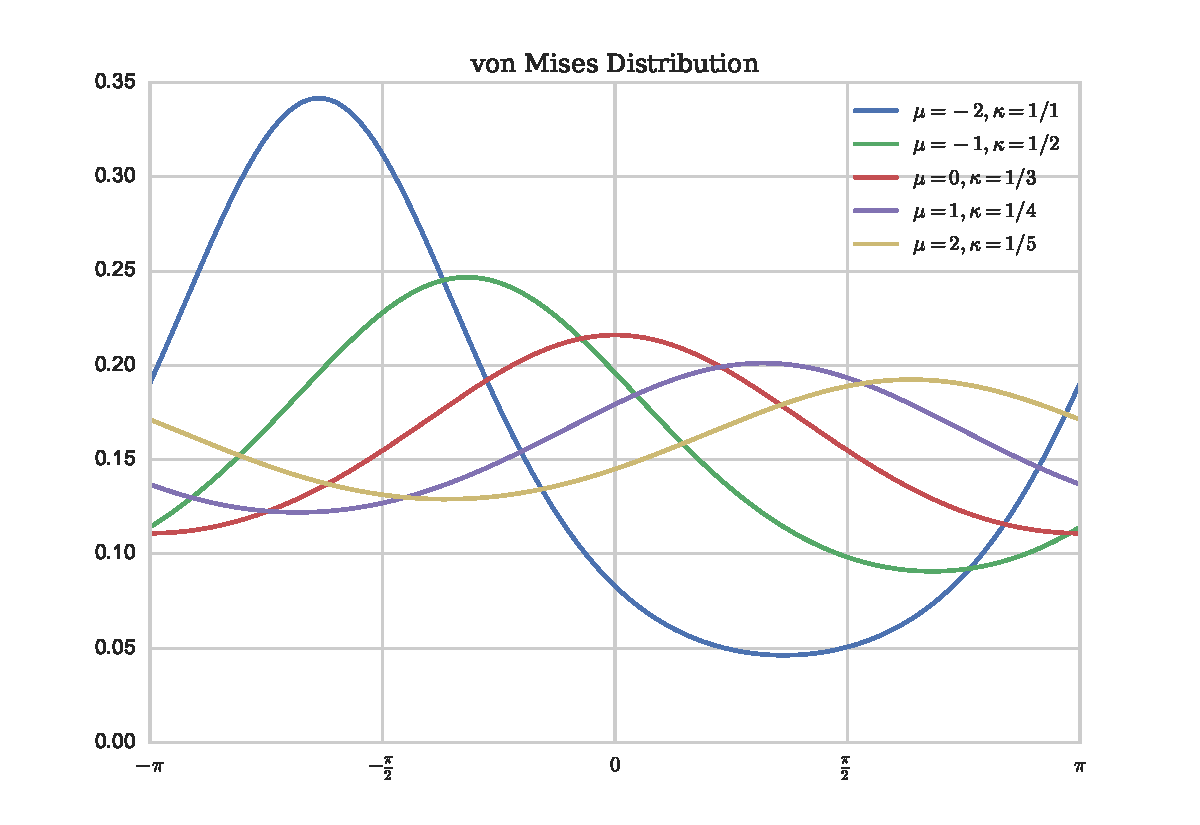
\includegraphics[width=.75\linewidth]{vonmises_2}
	\captionof{figure}{von Mises distribution for a variety of parameters}
	\label{fig:vonmises}
\end{figure}

\subsection{Joint Length-Orientation Distribution}
\label{sec:dist_2d}
The previous two distributions can reasonably be assumed to be independent of one another. That is, the angle of the frond does not depend on the length, or vice versa.
Therefore, the probability of a frond simultaneously having a given frond length and angle is the product of their individual probabilities.

Given independent events $A$ and $B$,
\begin{equation*}
	\label{eq:ind_prob}
	P(A \cap B) = P(A)P(B)
\end{equation*}
Then the probability of frond length $l$ and frond angle $\theta_f$ coinciding is 
\begin{equation*}
	P_{2D}(\theta_f,l) = P_{\theta_f}(\theta_f) \cdot P_l(l)
\end{equation*}
A contour plot of this 2D distribution for a specific set of parameters is shown in Figure \ref{fig:dist_2d}, where probability is represented by color in the 2D plane.
Darker green represents higher probability, while lighter beige represents lower probability.
In Figure \ref{fig:kelp_sample}, 50 samples are drawn from this distribution and plotted.

It is important to note that if $P_{\theta_f}$ were dependent on $l$, the above definition of $P_{2D}$ would no longer be valid.
For example, it might be more realistic to say that larger fronds are less likely to bend towards the direction of the current.
In this case, \eqref{eq:ind_prob} would no longer hold, and it would be necessary to use the more general relation
\begin{equation*}
	P(A \cap B) = P(A)P(B|A) = P(B)P(B|A),
\end{equation*}
which is currently not taken into consideration in this model.

\begin{figure}[h]
	\centering
	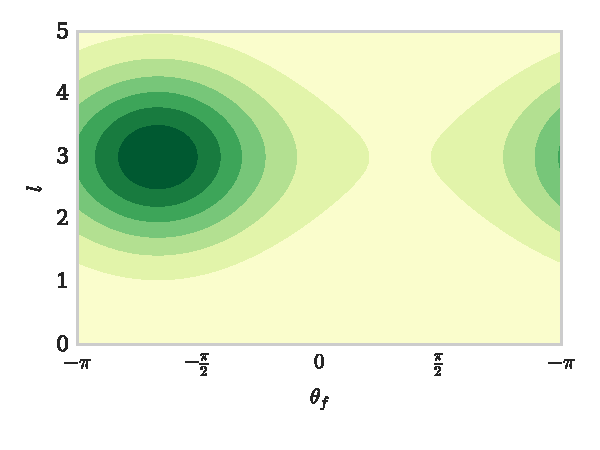
\includegraphics[width=.75\linewidth]{prob_2d}
	\vspace{-3em}
	\captionof{figure}{2D length-angle probability distribution with $\theta_w=2\pi/3,v_w=1$}
	\label{fig:dist_2d}
\end{figure}

\begin{figure}[h]
	\centering
	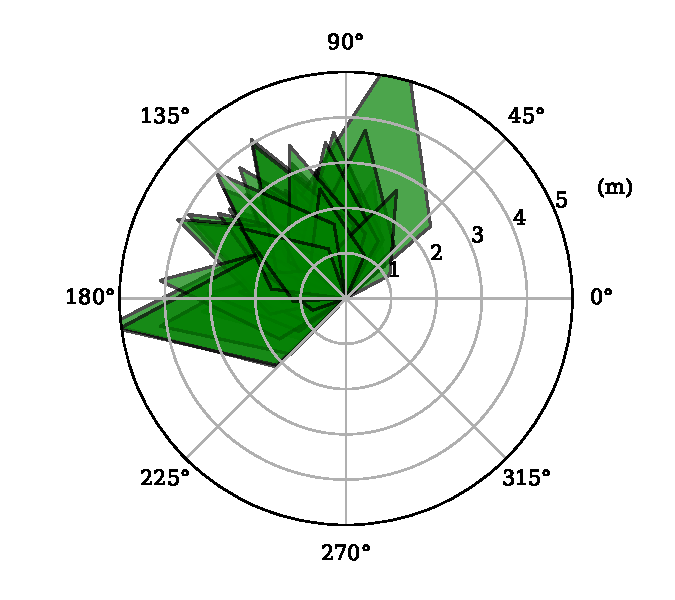
\includegraphics[width=.75\linewidth]{kelp_sample}
	\vspace{-2em}
	\captionof{figure}{A sample of 50 kelp fronds with length and angle picked from the distribution above with $f_s=0.5$ and $f_r=2$.}
	\label{fig:kelp_sample}
\end{figure}

\section{Spatial Distribution}
\subsection{Rotated Coordinate System}
\label{sec:rot_coords}
To determine under what conditions a frond will occupy a given point, we begin by
describing the shape of the frond in Cartesian coordinates and then convert to polar coordinates.
Of primary interest are the edges connected to the frond tip.
For convenience, we will use a rotated coordinate system $(\theta',s)$ such that the line connecting the base to the tip is vertical, with the base at $(0,0)$.
Denote the Cartesian analogue of this coordinate system as $(x',y')$ which is related to $(\theta',s)$ by
\begin{align*}
	x' &= s\cos\theta' \\ 
	y' &= s\sin\theta' \\
	s &= \sqrt{x'^2+y'^2}, \\
	\theta' &= \atantwo(y, x).
\end{align*}

\subsection{Functional Description of Frond Edge}
With this coordinate system established, the outer two edges of the frond can be described in Cartesian coordinates as a piecewise linear function connecting the left corner: $(-w/2,f_a)$, the tip: $(0,l)$, and the right corner: $(w/2,f_a)$.
This function has the form
\begin{equation*}
	y'_f(x') = l-\sign(x')\frac{f_b}{w/2}x'.
\end{equation*}
Using the equations in Section \ref{sec:rot_coords}, this can be written in polar coordinates after some rearrangement as
\begin{equation*}
	s_f'(\theta') = \frac{l}{\sin\theta' + S(\theta')\frac{2f_b}{w}\cos\theta'},
\end{equation*}
where
\begin{equation*}
	S(\theta') = \sign(\theta'-\pi/2).
\end{equation*}
Then, using the relationships in Section \ref{sec:shape}, the above equation can be rewritten in terms of the frond ratios $f_s$ and $f_r$ as
\begin{equation*}
	\label{eq:rf_rel}
	s_f'(\theta') = \frac{l}{\sin\theta' + S(\theta')\frac{2f_r}{1+f_s}\cos\theta'}.
\end{equation*}
To generalize to a frond pointed at an angle $\theta_f$, we introduce the coordinate system $(\theta,s)$ such that
\begin{equation*}
	\theta = \theta' + \theta_f - \frac{\pi}{2}
\end{equation*}
Then, for a frond pointed at the arbitrary angle $\theta_f$, the function for the outer edges can be written as 
\begin{equation*}
	\label{eq:rf_abs}
	s_f(\theta) = s_f'\left(\theta - \theta_f + \frac{\pi}{2} \right).
\end{equation*}

\subsection{Conditions for Occupancy}
We now formulate the conditions under which a kite shape frond occupies a point
in the sense that the point lies within its interior.
Combining these conditions with the size and orientation distributions from \ref{sec:dist}
allows a spatial distribution of the kelp fronds to be calculated.

Consider a fixed frond of length $l$ at an angle $\theta_f$. The point
$(\theta,s)$ is occupied by the frond if
\begin{align*}
	\left|\theta_f - \theta \right| < \alpha,
	s < s_f(\theta).
\end{align*}

Equivalently, the opposite perspective can be taken.
Letting the point $(\theta,s)$ be fixed, a frond occupies the point if
\begin{align}
	\theta - \alpha < \theta_f < \theta + \alpha,
	\label{eqn:rs_th} \\
	l > l_{min}(\theta,s),
	\label{eqn:rs_l}
\end{align}
where
\begin{equation*}
	l_{min}(\theta,s) = s \cdot \frac{l}{s_f(\theta)}.
\end{equation*}
Then, considering the point to be fixed, \eqref{eqn:rs_th} and \eqref{eqn:rs_l} define the spacial region $R_s(\theta,s)$ called the ``occupancy region for $(\theta,s)$'' with the property that if the tip of a frond lies within this region (i.e., $(\theta_f,l) \in R_s(\theta,s)$), then it occupies the point.
$R_s(3\pi/4,3/2)$ is shown in blue in Figure \ref{fig:shade_area} and the smallest possible occupying fronds for several values of $\theta_f$ are shown in various colors.
Any frond longer than these at the same angle will also occupy the point.

\begin{figure}[h]
	\centering
	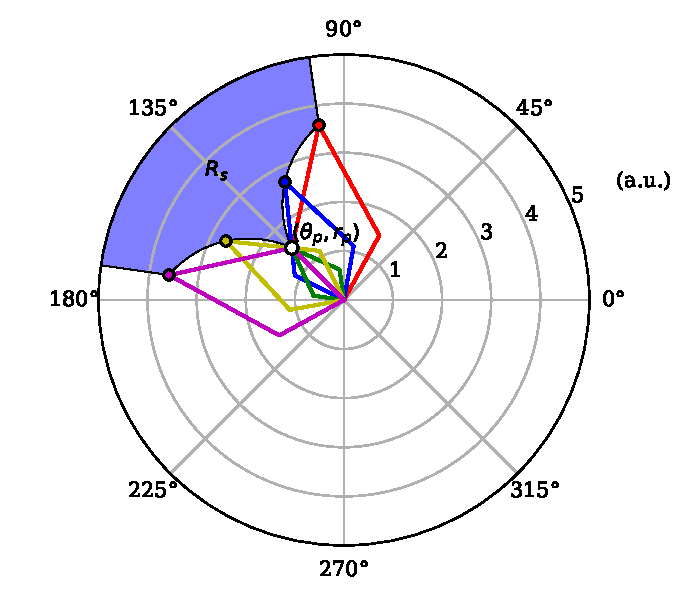
\includegraphics[width=.75\linewidth]{shade_area}
	\vspace{-2em}
	\captionof{figure}{Outlines of minimum-length fronds for a variety of angles to occupy the point $(\theta,s)=(3\pi/4,3/2)$}
	\label{fig:shade_area}
\end{figure}

\subsection{Probability of Occupancy}
We are interested in the probability that, given a fixed point $(\theta,s)$, values of $l$ and $\theta_f$ chosen from the distributions described in Section \ref{sec:dist} will fall in the occupancy region.
This is found by integrating $P_{2D}$ over the occupancy region for $(\theta,s)$.

\begin{figure}[H]
	\centering
	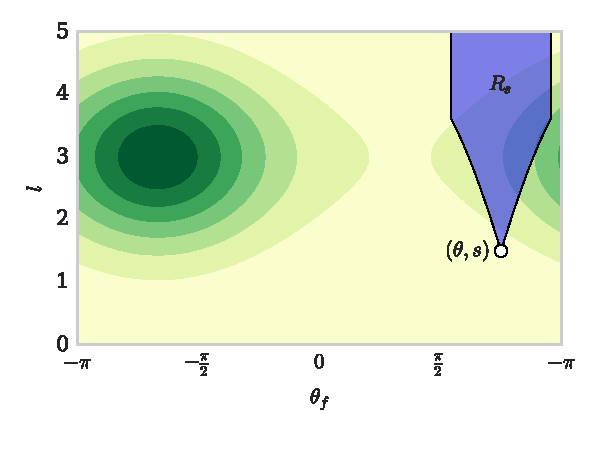
\includegraphics[width=.75\linewidth]{cart_shade}
	\vspace{-3em}
	\captionof{figure}{Contour plot of $P_{2D}(\theta_f,l)$ overlayed with the
    region in the $\theta_f-l$ plane which results in a frond occupying the point $(\theta,s)=(3\pi/4,3/2)$}
	\label{fig:cart_shade}
\end{figure}

Integrating $P_{2D}(\theta_f,l)$ over $R_s(\theta,s)$ as depicted in Figure \ref{fig:cart_shade} yields the proportion of the population occupying the point $(\theta,s)$,
\begin{align*}
		\tilde{P}_k(\theta,s,z)	&= \iint_{R_s(\theta,s)}
								P_{2D}(\theta_f,l)
								\,dl\,d\theta_f \nonumber \\
							&= \int_{\theta-\alpha}^{\theta+\alpha} 
								\int_{l_{min}(\theta_f)}^\infty
								P_{2D}(\theta_f,l)
								\,dl\,d\theta_f.
\end{align*}

Then, multiplying $\tilde{P}_k$ by the number of fronds in the population $n$ of the depth layer gives the expected number of fronds occupying the point.
Assuming a uniform thickness $t$ for all fronds, and a thickness $dz$ of the depth layer, the proportion of the grid cell occupied by kelp is found to be
\begin{equation*}
  P_k = \frac{nt}{dz}\tilde{P}_k.
\end{equation*}

Then, the effective absorption coefficient can be calculated at any point in space as
\begin{equation*}
  a(\vec{x}) = P_k(\vec{x})a_k + (1-P_k(\vec{x}))a_w
\end{equation*}

\begin{figure}[h]
	\centering
	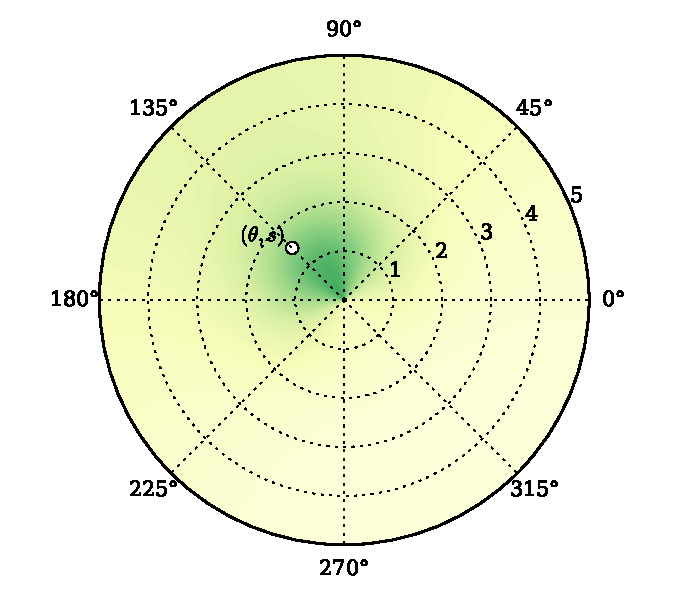
\includegraphics[width=.75\linewidth]{prob_shade}
	\vspace{-2em}
	\captionof{figure}{Colored plot of the probability of frond occupation sampled at 121 points using $\theta_f=2\pi/3,v_w=1$}
	\label{fig:prob_shade}
\end{figure}
 \chapter{LIGHT MODEL}
\label{chap:light}

Now that we have formulated the distribution of kelp throughout the medium, we introduce the Radiative Transfer Equation, which is used to calculate the light field.

\section{Optical Definitions}

\subsection{Radiometric Quantities}

One of the most fundamental quantities in optics is radiant flux $\Phi$, which is the has units of energy per time.
The quantity of primary interest in modeling the light field is radiance $L$, which is defined as the radiant flux per steradian per projected surface area perpendicular to the direction of propagation of the beam.
That is,

\begin{equation*}
	L = \frac{d^2\Phi}{dA d\vec{\omega}}
\end{equation*}

Once the radiance $L$ is calculated everywhere, the irradiance is
\begin{equation*}
  I(\vec{x}) = \int_{4\pi}L(\vec{x},\vec{\omega})\, d\vec{\omega}.
\end{equation*}
Integrating $I(\vec{x})$, which has units \SI{}{\W/m^2}, over the surface of a frond, produces the power (with units \SI{}{\W}) transmitted to the frond.
For details, see Section \ref{sec:perceived_irrad}.

Irradiance is sometimes given in units of moles of photons (a mole of photons is also called an Einstein) per second, with the conversion \cite{mobley_light_1994} given by
\begin{equation}
  \SI{1}{\W\per\m^2} = \SI{4.2}{\micro\mole \,photons\per\second}.
  \label{eqn:watts_photons}
\end{equation}

\subsection{Perceived Irradiance}
\label{sec:perceived_irrad}

The average irradiance experienced by a kelp frond in depth layer $k$ is
\newcommand{\Iperk}{\tilde{I}_k}
\begin{equation*}
   \Iperk = \frac{\sum_{ij}P_{ijk}I_{ijk}}{\sum_{ij}P_{ijk}}.
\end{equation*}

The irradiance perceived by the kelp is expected to be slightly lower than the average irradiance,
\begin{equation*}
  \bar{I}_k = \frac{\sum_{ij}I_{ijk}}{n_x n_y}
\end{equation*}
since the kelp is more densely located at the center of the domain where the light field is reduced,
whereas the simple average is influenced by regions of higher irradiance at the edges of the domain where kelp is not present.

\subsection{Inherent Optical Properties}
We must now define a few inherent optical properties (IOPs) which depend only on the medium of propagation.
These phenomena are governed by three inherent optical properties (IOPs) of the
medium.
The absorption coefficient $a(\vec{x})$ (units m$^{-1}$) defines the
proportional loss of radiance per unit length.
The scattering coefficient $b$ (units m$^{-1}$), defines the proportional loss
of radiance per unit length, and is assumed to be constant over space.

The volume scattering function (VSF) $\beta(\Delta): [-1, 1] \to \RR^+$ (units sr$^{-1}$) defines the probability of light scattering at any given angle from its source.
Formally, given two directions $\vec{\omega}$ and $\vec{\omega}'$, $\beta(\vec{\omega} \cdot \vec{\omega}')$ is the probability density of light scattering from $\vec{\omega}$ into $\vec{\omega}'$ (or vice-versa).
Of course, since a single direction subtends no solid angle, the probability of scattering occurring exactly from $\vec{\omega}$ to $\vec{\omega}'$ is 0.
Rather, we say that the probability of radiance being scattered from a direction $\omega$ into an element of solid angle $\Omega$ is $\int_\Omega \beta(\vec{\omega} \cdot \vec{\omega}')\, d\vec{\omega}'$.

The VSF is normalized such that
\begin{equation*}
  \int_{-1}^1\beta(\Delta)\, d\Delta=\frac{1}{2\pi},
\end{equation*}
so that for any $\omega$,
\begin{equation*}
  \int_{4\pi}\beta(\vec{\omega}\cdot\vec{\omega}')\, d\vec{\omega}' = 1.
\end{equation*}
i.e., the probability of light being scattered to some direction on the unit sphere is 1.


\section{The Radiative Transfer Equation}
We now present the Radiative Transfer Equation, whose solution is the radiance in the medium as a function of position and angle.

\subsection{Ray Notation}
Consider a fixed position $\vec{x}$ and direction $\vec{\omega}$ such that
$\vec{\omega} \cdot \hat{z} \neq 0$.
Let $\vec{l}(\vec{x}, \vec{\omega}, s)$ denote the linear path containing $\vec{x}$ in the direction $\vec{\omega}$.
Assume that the ray is not horizontal.
Then, it originates either at the surface or bottom of the domain, with initial z coordinate given by
\begin{equation*}
  z_0 =
   \begin{cases}
    0, & \vec{\omega} \cdot \hat{z} < 0 \\
    \zmax, & \vec{\omega} \cdot \hat{z} > 0.
  \end{cases}
\end{equation*}
Hence, the ray path is parameterized as
\begin{equation}
  \vec{l}(\vec{x}, \vec{\omega}, s) = \frac{1}{\tilde{s}} (s\vec{x} + (\tilde{s} - s)\vec{x_0}(\vec{x}, \vec{\omega})),
  \label{eqn:ray_path}
\end{equation}
where
\begin{equation*}
  \vec{x_0}(\vec{x}, \vec{\omega}) = \vec{x} - \tilde{s} \vec{\omega}
\end{equation*}
is the origin of the ray, and 
\begin{equation*}
  \tilde{s} = \frac{\vec{x} \cdot \hat{z} - z_0}{\vec{\omega} \cdot \hat{z}}
\end{equation*}
is the path length from $\vec{x_0}(\vec{x}, \vec{\omega})$ to $\vec{x}$.

\subsection{Colloquial Description}
Denote the radiance at $\vec{x}$ in the direction $\vec{\omega}$ by $L(\vec{x}, \vec{\omega})$.
As light travels along $\vec{l}(\vec{x}, \vec{\omega}, s)$, interaction with the
medium produces three phenomena of interest:
\begin{enumerate}
  \item Radiance is decreased due to absorption.
  \item Radiance is decreased due to scattering out of the path to other
    directions.
  \item Radiance is increased due to scattering into the path from other
      directions.
\end{enumerate}

\subsection{Equation of Transfer}
Combining these phenomena yields the Radiative Transfer Equation along
$\vec{l}(\vec{x}, \vec{\omega})$,
\begin{equation}
  \label{eqn:rte1d}
  \frac{dL}{ds}(\vec{l}(\vec{x}, \vec{\omega}, s), \vec{\omega})
  = -(a(\vec{x}) + b)L(\vec{x}, \vec{\omega})
  + b \int_{4\pi} \beta(\vec{\omega}\cdot\vec{\omega}') L(\vec{x})\, d\vec{\omega}',
\end{equation}
where $\int_{4\pi}$ denotes integration over the unit sphere.
The derivative of $L$ over the path can be rewritten as
\begin{align*}
  \frac{dL}{ds}(\vec{l}(\vec{x}, \vec{\omega}, s), \vec{\omega})
    &= \frac{d\vec{l}}{ds}(\vec{x}, \vec{\omega}, s) \cdot \nabla L(\vec{x}, \vec{\omega}', \vec{\omega}) \\
    &= \vec{\omega} \cdot \nabla L(\vec{x}, \vec{\omega}),
\end{align*}
which unveils the general form of the Radiative Transfer Equation,
\begin{equation*}
  \vec{\omega} \cdot \nabla L(\vec{x}, \vec{\omega})
  = -(a(\vec{x}) + b)L(\vec{x}, \vec{\omega})
  + b \int_{4\pi} \beta(\vec{\omega}\cdot\vec{\omega}') L(\vec{x}, \vec{\omega}')\, d\vec{\omega}'
\end{equation*}

or, equivalently,
\begin{equation}
  \vec{\omega} \cdot \nabla L(\vec{x}, \vec{\omega})
  + a(\vec{x})L(\vec{x}, \vec{\omega})
  = b \left(
    \int_{4\pi} \beta(\vec{\omega}\cdot\vec{\omega}') L(\vec{x}, \vec{\omega}')\, d\vec{\omega}'
    - L(\vec{x}, \vec{\omega})
  \right).
  \label{eqn:rte}
\end{equation}

\subsection{Boundary Conditions}

We use periodic boundary conditions in the $x$ and $y$ directions,
\begin{align*}
  L\left((\xmin, y, z), \vec{\omega}\right) &= L\left((\xmax, y, z), \vec{\omega}\right), \\
  L\left((x, \ymin, z), \vec{\omega}\right) &= L\left((x, \ymax, z), \vec{\omega}\right).
\end{align*}
In the $z$ direction, we specify a spatially uniform downwelling light just
under the surface of the water by a function $f(\vec{\omega})$.
Or if $\zmin>0$, then the radiance at $z=\zmin$ should be specified instead (as opposed to the radiance at the first grid cell center).
Further, we assume that no upwelling light enters the domain from the bottom, so
\begin{align*}
  L(\vec{x_s}, \vec{\omega}) &= f(\omega) \mbox{ if } \vec{\omega} \cdot \hat{z} > 0, \\ 
  L(\vec{x_b}, \vec{\omega}) &= 0 \mbox { if } \vec{\omega} \cdot \hat{z} < 0.
\end{align*}
 
\section{Low-Scattering Approximation}
In clear waters where absorption is more important than scattering, an asymptotic expansion can be used whereby the light field is generated through a sequence of discrete scattering events.
\subsection{Asymptotic Expansion}
Taking $b$ to be small, we introduce the asymptotic series
\newcommand{\Lasym}{L_0(\vec{x},\vec{\omega}) + b L_1(\vec{x},\vec{\omega}) + b^2 L_2(\vec{x},\vec{\omega}) + \cdots}
\newcommand{\Lasyms}{L_0(\vec{x_s},\vec{\omega}) + b L_1(\vec{x_s},\vec{\omega}) + b^2 L_2(\vec{x_s},\vec{\omega}) + \cdots}
\newcommand{\Lasymp}{L_0(\vec{x},\vec{\omega}') + b L_1(\vec{x},\vec{\omega}') + b^2 L_2(\vec{x},\vec{\omega}') + \cdots}
\begin{align*}
  L(\vec{x},\vec{\omega}) = \Lasym.
\end{align*}
Substituting the above into \eqref{eqn:rte} yields
\begin{align*}
    &\vec{\omega} \cdot \nabla \left[ \Lasym \right] \\
    &+ a(\vec{x}) \left[ \Lasym \right] \\
    &= b\Bigg(
      \int_{4\pi} \beta(\vec{\omega}\cdot\vec{\omega}')
      \left[ \Lasymp \right] \, d\vec{\omega}' \\
    &- \left[ \Lasym \right]
    \Bigg).
\end{align*}
Grouping like powers of $b$, we have the decoupled set of equations
\begin{align}
  \vec{\omega} \cdot \nabla L_0(\vec{x}, \vec{\omega}) + a(\vec{x})L_0(\vec{x}) &= 0,
  \label{eqn:asymptotics_0}\\
  \vec{\omega} \cdot \nabla L_1(\vec{x}, \vec{\omega}) + a(\vec{x})L_1(\vec{x})
  &= \int_{4\pi} \beta(\vec{\omega}\cdot\vec{\omega}') L_0(\vec{x}, \vec{\omega}')\,d\vec{\omega}' - L_0(\vec{x}, \vec{\omega}), \nonumber\\ 
  \vec{\omega} \cdot \nabla L_2(\vec{x}, \vec{\omega}) + a(\vec{x})L_2(\vec{x})
  &= \int_{4\pi} \beta(\vec{\omega}\cdot\vec{\omega}') L_1(\vec{x}, \vec{\omega}')\,d\vec{\omega}' - L_1(\vec{x}, \vec{\omega}). \nonumber \\ 
  &\vdots \nonumber
\end{align}
In general, for $n \geq 1$,
\begin{equation}
  \vec{\omega} \cdot \nabla L_n(\vec{x}, \vec{\omega}) + a(\vec{x})L_n(\vec{x})
  = \int_{4\pi} \beta(\vec{\omega}\cdot\vec{\omega}') L_{n-1}(\vec{x}, \vec{\omega}')\,d\vec{\omega}' - L_{n-1}(\vec{x}, \vec{\omega}).
  \label{eqn:asymptotics_n}
\end{equation}

For boundary conditions, let $\vec{x_s}$ be a point on the surface of the domain.
Then, 
\begin{equation*}
  \Lasyms =
  \begin{cases}
    f(\omega), & \hat{z}\cdot\omega > 0 \\
    0, & \mbox{otherwise},
  \end{cases}
\end{equation*}
which can be decomposed as
\begin{align}
  L_0(\vec{x}, \vec{\omega}) &=
  \begin{cases}
    f(\omega), & \hat{z}\cdot\omega > 0, \\
    0, & \mbox{otherwise},
  \end{cases}
  \label{eqn:asymptotics_bc_0} \\
  L_1(\vec{x}, \vec{\omega}) &= 0 \nonumber \\
  L_2(\vec{x}, \vec{\omega}) &= 0. \nonumber \\
  &\vdots \nonumber
\end{align}
In general, for $n \geq 1$,
\begin{equation}
  L_n(\vec{x}, \vec{\omega}) = 0.
  \label{eqn:asymptotics_bc_n}
\end{equation}

 
\subsection{Analytical Solution}
\label{sec:asymptotic_sol}

For all $\vec{x}, \vec{\omega}$, we consider the path $l(\vec{x}, \vec{\omega}, s)$ from \eqref{eqn:ray_path}.
We extract the absorption coefficient along the path,
\begin{equation*}
  \tilde{a}(s) = a(\vec{l}(\vec{x}, \vec{\omega}), s).
\end{equation*}
Then, the first equation from the asymptotic expansion, \eqref{eqn:asymptotics_0} and its associated boundary condition, \eqref{eqn:asymptotics_bc_0}, can be rewritten as
\begin{equation*}
  \left\{
  \begin{aligned}
  0 &= \frac{du_0}{ds}(s) + \tilde{a}(s) u_0(s) \\
  u_0(0) &= f(\vec{\omega}),
  \end{aligned}
  \right.
\end{equation*}
which we can solve by multiplying by the appropriate integrating factor, as follows.
\begin{align*}
  0 &= \exp\left(\int_0^s \tilde{a}(s')\, ds'\right) \frac{du_0}{ds} + \exp\left(\int_0^s \tilde{a}(s')\, ds'\right) \tilde{a}(s) u_0(s) \\
  &= \frac{d}{ds}\left[\exp\left(\int_0^s \tilde{a}(s')\, ds'\right) u_0(s)\right].
\end{align*}
Then, integrating both sides yields
\begin{align*}
  0 &= \int_0^s \frac{d}{ds'}\left[\exp\left(\int_0^{s'} \tilde{a}(s'')\, ds''\right) u_0(s')\right]\, ds' \\
  &= \exp\left(\int_0^s \tilde{a}(s')\, ds'\right) u_0(s) - f(\vec{\omega}).
\end{align*}
Hence,
\begin{equation}
  u_0(s) = f(\omega) \exp\left(-\int_0^s \tilde{a}(s)\, ds\right).
  \label{eqn:asymptotics_soln_0}
\end{equation}
Then, we convert back from path length $s$ to the spatial coordinate $\vec{x}$ using
\begin{equation*}
  L_0(\vec{l}(\vec{x}, \vec{\omega},s), \vec{\omega}) = u_0(s).
\end{equation*}

The $n \geq 1$ equations have a nonzero right-hand side, which we call the effective source, $g_n(s)$.
This can be similarly extracted along a ray path as
\begin{equation*}
  g_n(s) = \int_{4\pi} \beta(\vec{\omega}\cdot\vec{\omega}')
  L_{n-1}(\vec{l}(\vec{x}, \vec{\omega'}, s), \vec{\omega}')\,d\vec{\omega}' - L_{n-1}(\vec{l}(\vec{x}, \vec{\omega}, s), \vec{\omega}).
\end{equation*}
Then, since $g_n$ depends only on $L_{n-1}$, it is independent of $u_n$, which allows \eqref{eqn:asymptotics_n} and its boundary condition, \eqref{eqn:asymptotics_bc_n}, to be written as the first order, linear ordinary differential equation along the ray path,
\begin{equation*}
  \left\{
  \begin{aligned}
    g_n(s) &= \frac{du_n}{ds}(s) + \tilde{a}(s)u_n(s) \\
    u_n(0) &= 0
  \end{aligned}
  \right.
\end{equation*}
As with the $n=0$ equation, the solution is found by multiplying by the appropriate integrating factor.
\begin{align*}
  \exp\left(\int_0^s \tilde{a}(s')\, ds'\right) g_n(s) &= \exp\left(\int_0^s \tilde{a}(s')\, ds'\right) \frac{du_n}{ds} + \exp\left(\int_0^s \tilde{a}(s')\, ds'\right) \tilde{a}(s) u_n(s) \\
  &= \frac{d}{ds}\left[\exp\left(\int_0^s \tilde{a}(s')\, ds'\right) u_n(s)\right].
\end{align*}
Integrating both sides yields
\begin{align*}
  \int_0^s\exp\left(\int_0^{s'} \tilde{a}(s'')\, ds''\right) g_n(s')\, ds' &= \int_0^s \frac{d}{ds'}\left[\exp\left(\int_0^{s'} \tilde{a}(s'')\, ds''\right) u_n(s')\right]\, ds' \\
  &= \exp\left(\int_0^s \tilde{a}(s')\, ds'\right) u_n(s).
\end{align*}
Hence,
\begin{equation*}
  u_n(s) = \exp\left(-\int_0^s \tilde{a}(s')\, ds'\right) \int_0^s\exp\left(\int_0^{s'} \tilde{a}(s'')\, ds''\right) g_n(s')\, ds',
\end{equation*}
which simplifies to
\begin{equation}
  u_n(s) = \int_0^sg_n(s')\exp\left( -\int_{s''}^{s'}\tilde{a}(s'')\,ds'' \right)\, ds'.
  \label{eqn:asymptotics_soln_n}
\end{equation}
As before, the conversion back to spatial coordinates is
\begin{equation*}
  L_n(\vec{l}(\vec{x}, \vec{\omega}, s), \vec{\omega}) = u_n(s).
\end{equation*}
 \chapter{NUMERICAL SOLUTION}
\label{chap:numerical}

In this chapter, the mathematical details involved in the numerical solution of the previously described equations are presented.
It is assumed that this model is run in conjunction with a model describing the growth of kelp over its life cycle, which calls this light model periodically to update the light field.

\section{Super-Individuals}
\label{sec:si}

Rather than model each kelp frond, a subset of the population, called super-individuals, are modeled explicitly, and are considered to represent many identical individuals, as in \citep{scheffer_super-individuals_1994}.
Specifically, at each depth $k$, there are $n$ super-individuals, indexed by $i$.
Super-individual $i$ has a frond area $A_{ki}$ and represents $n_{ki}$ individual fronds.

From \eqref{eqn:length-from-area}, the frond length of the super-individual is $l_{ki} = \sqrt{2A_{ki}f_r}$.
Given the super-individual data, we calculate the mean $\mu$ and standard deviation $\sigma$ frond
lengths using the formulas
\begin{align}
  \mu_k &= \frac{\ds \sum_{i=1}^N l_{ki}}{\ds \sum_{i=1}^N n_{ki}},
  \label{eqn:si_mean} \\
  \sigma_k &= \frac{\ds \sum_{i=1}^N \left( l_{ki} - \mu_k \right)^2}{\ds \sum_{i=1}^N n_{ki}}.
  \label{eqn:si_std}
\end{align}
We then assume that frond lengths are normally distributed in each depth layer
with mean $\mu_k$ and standard deviation $\sigma_k$.

\section{Discrete Grid}
\label{sec:grid}

The following is a description of the spatial-angular grid used in the numerical implementation of this model.
It is assumed that all simulated quantities are constant over the interior of a grid cell.
Other legitimate choices of grids exists; this one was chosen for its relative simplicity.

The domain of the radiative transfer equation is embedded in five dimensions: three spatial ($x$, $y$, and $z$) and two angular (azimuthal $\theta$ and polar $\phi$).
The number of grid cells in each dimension are denoted by $n_x$, $n_y$, $n_z$,
$n_\theta$, and $n_\phi$, with uniform spacings $dx$, $dy$, $dz$, $d\theta$, and
$d\phi$ between adjacent grid points.

The following indices are assigned to each dimension:
\begin{align*}
  x &\to i \\
  y &\to j \\
  z &\to k \\
  \theta &\to l \\
  \phi &\to m
\end{align*}

It is convenient, however, to use a single index $p$ to refer to directions $\vec{\omega}$ rather than referring to $\theta$ and $\phi$ separately.
Then, the center of a generic grid cell will be denoted as
$(x_i, y_j, z_k, \vec{\omega}_p)$, and the boundaries between adjacent grid cells
will be referred to as \textit{edges}.
One-indexing is employed throughout this document.

\begin{figure}[H]
  \centering
  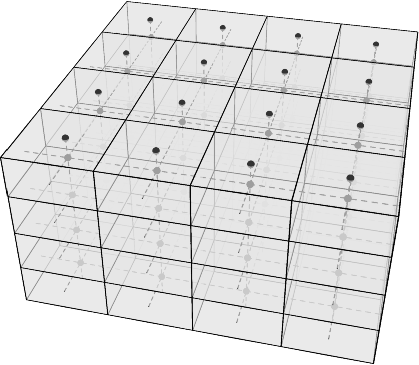
\includegraphics[width=8cm]{spatialgrid.pdf}
  \caption{Spatial grid}
  \label{fig:spatial_grid}
\end{figure}

Each spatial grid cell is the Cartesian product of $x$, $y$, and $z$ intervals of width $dx$, $dy$, and $dz$ respectively.
The three-dimensional interval centered at $(x_i, y_j, z_k)$ is denoted $X_{ijk}$, and has volume $\abs{X_{ijk}}=dx\,dy\,dz$.
Also, note that no grid center is located on the plane $z=0$; the surface radiance boundary condition is treated separately.

\begin{figure}[H]
  \centering
  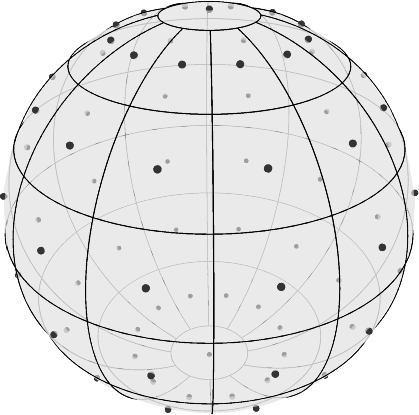
\includegraphics[width=8cm]{angulargrid.pdf}
  \caption{Angular grid at each point in space}
  \label{fig:angular_grid}
\end{figure}

As shown in Figure \ref{fig:angular_grid}, $\phi=0$ and $\phi=\pi$, called
the north ($+z$) and south ($-z$) poles respectively, are treated separately from other angular grid cells.
A generic interior angular grid cell centered at $\vec{\omega}_p$ is the Cartesian product of an azimuthal interval of width $d\theta$ and a polar interval of width $d\theta$.
However, two pole cells are the Cartesian product of a polar interval of width $d\phi/2$ and the full azimuthal domain, $[0, 2\pi)$.

With this configuration, the total number of angles considered is $\nomega = n_\theta(n_\phi-2)+2$.
Then, cells are indexed by $p=1,\ldots,n_{\vec{\omega}}$ and are ordered such that
$p=1$ and $p=n_{\vec{\omega}}$ refer to the north and south poles respectively,
$p\leq\nomega/2$ refers to the northern hemisphere, and $p>\nomega/2$ refers to the southern hemisphere.
Further, the symbol $\Omega_p$ is used to refer to the two dimension angular interval centered at $\omega_p$.
The solid angle subtended by $\Omega_p$ is denoted $\abs{\Omega_p}$.
Refer to Appendix \ref{chap:grid_details} for a more rigorous discussion of the discrete spatial-angular grid.

\section{Quadrature Rules}
Since it is assumed that all quantities are constant within a spatial-angular grid cell,
the midpoint rule is employed for both spatial and angular integration.
Presented here is a basic derivation of the formulas for integration in the spatial-angular grid.
Further details are found in Appendix \ref{chap:ray_tracing}.

\subsection{Spatial Quadrature}
Define the \textit{spatial characteristic function} as
\begin{equation*}
  \mathcal{X}^X_{ijk}(\vec{x}) = \begin{cases}
    1, & \vec{x} \in X_{ijk} \\
    0, & \mbox{otherwise}.
  \end{cases}
\end{equation*}
The double integral of a function $f(\vec{x})$ over a depth layer $k$ is approximated as
\begin{align*}
  \int_\xmin^\xmax\int_\ymin^\ymax f(x, y, z_k)\, dy\, dx &\approx \int_\xmin^\xmax \int_\ymin^\ymax \sum_{i=1}^{n_x}\sum_{j=1}^{n_y} \mathcal{X}^X_{ijk}(x,y,z_k) f(x_i, y_j, z_k)\, dy\, dx \\
  &= \sum_{i=1}^{n_x}\sum_{j=1}^{n_y} f(x_i, y_j, z_k) \int_\xmin^\xmax \int_\ymin^\ymax \mathcal{X}^X_{ijk}(x,y,z_k) \, dy\, dx \\
  &= \sum_{i=1}^{n_x}\sum_{j=1}^{n_y} \abs{X_{ijk}} f(x_i, y_j, z_k) \\
  &= dx\, dy\, dx\, \sum_{i=1}^{n_x}\sum_{j=1}^{n_y} f(x_i, y_j, z_k).
\end{align*}
The path integral of $f(\vec{x})$ over a path $\vec{l}(s)$ from $s=0$ to $s=\tilde{s}$ is
\begin{align*}
  \int_0^{\tilde{s}} f(\vec{l}(s))\, ds &= \sum_{i=1}^{n_x}\sum_{j=1}^{n_y}\sum_{k=1}^{n_z} f(x_i, y_j, z_k)\, ds_{ijk},
\end{align*}
where $ds_{ijk}$ is the total path distance of $\vec{l}(s)$ through $X_{ijk}$.
Full details of the path integral algorithm for the case of straight line paths are found in Appendix \ref{chap:ray_tracing}.

\subsection{Angular Quadrature}
Define the \textit{angular characteristic function} as
\begin{equation*}
  \mathcal{X}^\Omega_p(\vec{\omega}) = \begin{cases}
    1, & \vec{\omega} \in \Omega_p \\
    0, & \mbox{otherwise}.
  \end{cases}
\end{equation*}


Then, the integral of a function $f(\vec{\omega})$ is approximated as
\begin{align*}
  \int_{4\pi} f(\vec{\omega})\, d\vec{\omega} &\approx \int_{4\pi} \sum_{p=1}^\nomega f(\vec{\omega}_p) \mathcal{X}^\Omega_p(\vec{\omega})\, d\vec{\omega} \\
  &= \sum_{p=1}^\nomega f(\vec{\omega}_p) \int_{4\pi} \mathcal{X}^\Omega_p(\vec{\omega})\, d\vec{\omega} \\
  &= \sum_{p=1}^\nomega f(\vec{\omega}_p) \int_{\Omega_p} d\vec{\omega} \\
  &= \sum_{p=1}^\nomega f(\vec{\omega}_p) \abs{\Omega_p}.
\end{align*}

\section{Numerical Asymptotics}
Presented here are details of the evaluation of the asymptotic approximations \eqref{eqn:asymptotics_soln_0} and \eqref{eqn:asymptotics_soln_n} to the raditiave transfer equation \eqref{eqn:rte}.

\subsection{Scattering Integral}

Specifically, the amount of light scattered between angular grid cells is found by integrating $\beta$ as follows.
Consider two angular grid cells, $\Omega$ and $\Omega'$.
Since $\beta(\vec{\omega}\cdot\vec{\omega}')$ is the probability density of scattering between $\vec{\omega}$ and $\vec{\omega}'$, the average probability density of scattering from $\vec{\omega} \in \Omega$ to $\vec{\omega}' \in \Omega'$ (or vice versa) is
\begin{equation*}
  \beta_{pp'} = \frac{1}{\abs{\Omega}\abs{\Omega'}} \int_\Omega\int_{\Omega'}\beta(\vec{\omega}\cdot\vec{\omega}')\, d\vec{\omega'}\, d\vec{\omega}.
\end{equation*}
Denote the radiance at $(x_i, y_j, z_k, \vec{\omega}_p)$ by $L_{ijkp}$.
Then, the total radiance scattered into $\Omega_p$ from $\Omega_{p'}$ is
\begin{align*}
  \int_{\Omega}\int_{\Omega'}\beta(\vec{\omega} \cdot \vec{\omega}')L(\vec{x},\vec{\omega}')\, d\vec{\omega}'\, d\vec{\omega}
  &= L_{ijkp'} \int_\Omega\int_{\Omega_{p'}} \beta(\vec{\omega} \cdot \vec{\omega}')\, d\vec{\omega}'\, d\vec{\omega} \\
  &= \beta_{pp'}\abs{\Omega}\abs{\Omega'}L_{ijkp'}.
\end{align*}
Hence, the average radiance scattered from $\Omega_{p'}$ into some $\vec{\omega} \in \Omega_p$ is $\beta_{pp'}\abs{\Omega'}L_{ijkp'}$.
Therefore, the radiance gain due to scattering into $\vec{\omega}_p$ from all other angles is
\begin{equation}
  \int_{4\pi}\beta(\vec{\omega_p}\cdot\vec{\omega_{p'}})L(\vec{x}, \vec{\omega}')\, d\vec{\omega} \approx \sum_{p=1}^\nomega \beta_{pp'}\abs{\Omega'}L_{ijkp}.
  \label{eqn:scatter_integral}
\end{equation}

\subsection{Ray Integral}
Given a position $\vec{x}$ and direction $\vec{\omega}$, a path through the discrete grid can be constructed using the ray tracing algorithm described in Appendix \ref{chap:ray_tracing}. 
Let $\nu=1,\ldots,N\nobreak-\nobreak1$ index the spatial grid cells traversed by the ray, and define the \textit{path-length characteristic function}
\begin{equation*}
  \mathcal{X}^l_\nu(s) = \begin{cases}
    1, & s_\nu \leq s < s_{\nu+1} \\
    0, & \mbox{otherwise}.
    \end{cases}
\end{equation*}
Then, the piecewise constant representations of the path absorption coefficient $\tilde{a}(s)$ and the effective source $g_n(s)$ from Section \ref{sec:asymptotic_sol} are
\begin{align*}
  g_n(s) &= \sum_{\nu=1}^{N-1}g_{n\nu}\mathcal{X}^l_\nu(s), \\
  \tilde{a}(s) &= \sum_{\nu=1}^{N-1}\tilde{a}_{\nu}\mathcal{X}^l_\nu(s).
\end{align*}

As the ray traverses the spatial grids, it crosses $N-2$ spatial grid edges.
Let the nondecreasing path lengths at which these crossings occur be denoted by
$\left\{s_\nu\right\}_{\nu=1}^{N}$, with the convention $s_1=0$ and $s_{N}=\tilde{s}$.
$\{s_\nu\}$ is not strictly increasing if the ray directly intersects a grid corner,
which means that multiple edges are traversed at the same path length.
Hence, for $\nu=1,\ldots,N-1$, the path lengths through each grid cell are
\begin{equation*}
  ds_\nu = s_{\nu+1} - s_\nu.
\end{equation*}
Given $s$, the index next edge crossing occurs at
\begin{equation*}
  \hat{\nu}(s) = \min\left\{ \nu \in \{1,\ldots,N\} : s_\nu>s \right\},
\end{equation*}
and the path length between $s$ and the next edge crossing is
\begin{equation*}
  \tilde{d}(s) = s_{\hat{\nu}(s)}-s.
\end{equation*}
Then, evaluating \eqref{eqn:asymptotics_soln_n} at $s=\tilde{s}$ is calculated as
\begin{align*}
  u_n(\tilde{s}) &= \int_0^{\tilde{s}}g_n(s')\exp\left( -\int_{s''}^{s'}\tilde{a}(s'')\,ds'' \right)\, ds' \\
  &= \int_0^{s_N} \sum_{\nu=1}^{N-1}g_{n\nu}\mathcal{X}^l_\nu(s') \exp\left( -\int_{s''}^{s'}\sum_{j=1}^{N-1}\tilde{a}_{j}\mathcal{X}^l_j(s'')\,ds'' \right)\, ds' \\
  &= \sum_{\nu=1}^{N-1}g_{n\nu}\int_0^{s_N} \mathcal{X}^l_\nu(s') \exp\left( -\sum_{j=1}^{N-1}\tilde{a}_{j}\int_{s''}^{s'}\mathcal{X}^l_j(s'')\,ds'' \right)\, ds' \\
  &= \sum_{\nu=1}^{N-1}g_{n\nu}\int_{s_\nu}^{s_{\nu+1}}  \exp\left(-\tilde{a}_{\hat{\nu}(s')-1}\tilde{d}(s') -\sum_{j=\hat{\nu}(s')}^{N-1}\tilde{a}_{j}ds_j\right)\, ds' \\
  &= \sum_{\nu=1}^{N-1}g_{n\nu}\int_{s_\nu}^{s_{\nu+1}}  \exp\left(-\tilde{a}_{\nu}(s_{\nu+1}-s') -\sum_{j=\nu+1}^{N-1}\tilde{a}_{j}ds_j\right)\, ds'.
\end{align*}
This integral is made straightforward by setting
\begin{equation*}
  b_\nu = -\tilde{a}_{\nu}s_{\nu+1} - \sum_{j=\nu+1}^{N-1}\tilde{a}_{j}ds_j,
\end{equation*}
which yields
\begin{align*}
  u_n(\tilde{s}) &= \sum_{\nu=1}^{N-1}g_{n\nu}\int_{s_\nu}^{s_{\nu+1}}  \exp\left(\tilde{a}_{\nu}s' + b_\nu\right)\, ds' \\
                 &= \sum_{\nu=1}^{N-1}g_{n\nu}e^{b_\nu}\int_{s_\nu}^{s_{\nu+1}}  \exp\left(\tilde{a}_{\nu}s'\right) ds'.
\end{align*}
Define the intermediate variable
\begin{align*}
  d_\nu &= \int_{s_\nu}^{s_{\nu+1}}  \exp\left(\tilde{a}_{\nu}s'\right)\, ds' \\
    &= \begin{cases}
    ds_\nu, & \tilde{a} = 0 \\
      \left( \exp(\tilde{a}_\nu s_{\nu+1}) - \exp(\tilde{a}_\nu s_\nu) \right)/\tilde{a}_\nu, & \mbox{otherwise},
    \end{cases}
\end{align*}
which permits the simple formula
\begin{equation}
  u_n(\tilde{s}) = \sum_{\nu=1}^{N-1} g_{n\nu}d_\nu e^{b_\nu}.
  \label{eqn:discrete_ray_integral}
\end{equation}

\section{Finite Difference}
While the asymptotic solution is valid in case of low scattering, a more general solution is obtained via finite difference, whereby the derivatives and integrals in the integro-partial differential equation are discretized to differences and sums and evaluated at each grid cell in order to construct a linear system of equations whose solution approximates that of the analytical equation.
The price of a general solution, however, is greatly increased computational cost, both in terms of memory and CPU usage.
Not only is it necessary to store a potentially huge sparse matrix in memory, but its construction can take enormous amounts of time.
Nonetheless, it is useful to have access to a general numerical solution, at least for verification of approximations if not for direct use in applications.

\subsection{Discretization}

For the spatial interior of the domain, we use the second order central difference formula (CD2) to approximate the derivatives, which is
\begin{equation*}
    \tag{CD2}
    f'(x) = \frac{f(x+dx)-f(x-dx)}{2dx} + \mathcal{O}(dx^3).
\end{equation*}

When applying the PDE on the upper or lower boundary, we use the forward and backward difference (FD2 and BD2) formulas respectively.
Omitting $\mathcal{O}(dx^3)$, we have
\begin{equation*}
    \tag{FD2}
    \label{eq:FD2}
    f'(x) = \frac{-3f(x)+4f(x+dx)-f(x+2dx)}{2dx}
\end{equation*}
\begin{equation*}
    \tag{BD2}
    \label{eq:BD2}
    f'(x) = \frac{3f(x)-4f(x-dx)+f(x-2dx)}{2dx}
\end{equation*}

For the upper and lower boundaries, we need an asymmetric finite difference
method.
In general, the Taylor Series of a function $f$ about $x$ is
\begin{equation*}
  f'(x+\varepsilon) = \sum_{n=1}^\infty \frac{f^{(n)}(x)}{n!} \varepsilon^n \\
\end{equation*}

Truncating after the first few terms, we have
\begin{equation}
  \label{eqn:afd1}
  f'(x+\varepsilon)  = f(x) + f'(x)\varepsilon + \frac{f''(x)}{2}\varepsilon^2 + \mathcal{O}(\varepsilon^3)
\end{equation}

Similarly, replacing $\varepsilon$ with $-\varepsilon/2$ we have
\begin{equation}
  \label{eqn:afd2}
  f'(x-\frac{\varepsilon}{2}) = f(x) - \frac{f'(x)\varepsilon}{2} + \frac{f''(x)\varepsilon^2}{8} + \mathcal{O}(\varepsilon^3).
\end{equation}

Rearranging \eqref{eqn:afd1} produces
\begin{equation}
  \label{eqn:afd3}
  f''(x)\varepsilon^2 = 2f(x+\varepsilon) - 2f(x) - 2f'(x)\varepsilon + \mathcal{O}(\varepsilon^3)
\end{equation}

Combining \eqref{eqn:afd2} with \eqref{eqn:afd3} gives
\begin{align*}
  \varepsilon f'(x) &= 2f(x) - 2f(x-\frac{\varepsilon}{2}) + f''(x)\frac{\varepsilon^2}{8} + \mathcal{O}(\varepsilon^3) \\
                    &= 2f(x) - 2f(x-\frac{\varepsilon}{2}) + \frac{f(x+\varepsilon)}{4} - \frac{f(x)}{4} - \frac{f'(x)\varepsilon}{4} + \mathcal{O}(\varepsilon^3) \\
                    &= \frac{4}{5}\left( 2f(x)-2f(x-\frac{\varepsilon}{2}) + \frac{f(x+\varepsilon)}{4} - \frac{f(x)}{4} \right) + \mathcal{O}(\varepsilon^3)
\end{align*}

Then, dividing by $\varepsilon$ gives
\begin{equation*}
  f'(x) = \frac{-8f(x-\frac{\varepsilon}{2}) + 7f(x) + f(x+\varepsilon)}{5\varepsilon} + \mathcal{O}(\varepsilon^2)
\end{equation*}

Similarly, substituting $\varepsilon \to -\varepsilon$, we have 
\begin{equation*}
  f'(x) = \frac{- f(x-\varepsilon) - 7f(x) + 8f(x+\frac{\varepsilon}{2})}{5\varepsilon} + \mathcal{O}(\varepsilon^2)
\end{equation*}


\subsection{Difference Equations}
\label{sec:difference_equations}


In general, we have

\begin{equation*}
  \vec{\omega} \cdot \nabla L_p = -(a+b) L_p + \sum_{p'=1}^{n_{\vec{\omega}}} \beta_{pp'}L_{p'}.
\end{equation*}

Then,
\begin{equation*}
  \vec{\omega} \cdot \nabla L_p + (a+b(1-\beta_{pp'}))L_p - \sum_{p'=1}^{n_{\vec{\omega}}} \beta_{pp'} L_{p'} = 0
\end{equation*}

Interior:
\begin{equation*}
  \begin{aligned}
    0 &= \frac{L_{i+1,jkp}-L_{i-1,jkp}}{2dx}\sin\hat{\phi}_p\cos\hat{\theta}_p \\
    &+ \frac{L_{i,j+1,kp}-L_{i,j-1,kp}}{2dy}\sin\hat{\phi}_p\sin\hat{\theta}_p \\
    &+ \frac{L_{ij,k+1,p}-L_{ij,k-1,p}}{2dz}\cos\hat{\phi}_p \\
    &+ (a_{ijk}+b(1-\beta_{pp'}))L_{ijkp}  - \sum_{p'=1}^{n_{\vec{\omega}}} \beta_{pp'} L_{ijkp'}
  \end{aligned}
\end{equation*}

Surface downwelling (BC):
\begin{equation*}
  \begin{aligned}
    0 &= \frac{L_{i+1,jkp}-L_{i-1,jkp}}{2dx}\sin\hat{\phi}_p\cos\hat{\theta}_p \\
    &+ \frac{L_{i,j+1,kp}-L_{i,j-1,kp}}{2dy}\sin\hat{\phi}_p\sin\hat{\theta}_p \\
    &+ \frac{-8f_p + 7L_{ijkp} + L_{ij,k+1,p}}{5dz}\cos\hat{\phi}_p \\
    &+ (a_{ijk}+b(1-\beta_{pp'}))L_{ijkp} \\
    &- \sum_{p'=1}^{n_{\vec{\omega}}} \beta_{pp'} L_{ijkp'}.
  \end{aligned}
\end{equation*}

Combining $L_{ijkp}$ terms on the left and moving the boundary condition to the
right gives

\begin{equation*}
  \begin{aligned}
    &\frac{L_{i+1,jkp}-L_{i-1,jkp}}{2dx}\sin\hat{\phi}_p\cos\hat{\theta}_p \\
    + &\frac{L_{i,j+1,kp}-L_{i,j-1,kp}}{2dy}\sin\hat{\phi}_p\sin\hat{\theta}_p \\
    + &\frac{L_{ij,k+1,p}}{5dz}\cos\hat{\phi}_p \\
    + &(a_{ijk}+b(1-\beta_{pp'}) + \frac{7}{5dz} \cos\hat{\phi}_p)L_{ijkp} \\
    - &\sum_{p'=1}^{n_{\vec{\omega}}} \beta_{pp'} L_{ijkp'} = \frac{8f_p}{5dz} \cos\hat{\phi}_p.
  \end{aligned}
\end{equation*}

Likewise for the bottom boundary condition, we have

\begin{equation*}
  \begin{aligned}
    0 &= \frac{L_{i+1,jkp}-L_{i-1,jkp}}{2dx}\sin\hat{\phi}_p\cos\hat{\theta}_p \\
    &+ \frac{L_{i,j+1,kp}-L_{i,j-1,kp}}{2dy}\sin\hat{\phi}_p\sin\hat{\theta}_p \\
    &- \frac{L_{ij,k-1,p}}{5dz}\cos\hat{\phi}_p \\
    &+ (a_{ijk}+b(1-\beta_{pp'}) - \frac{7}{5dz}\cos\hat{\phi}_p)L_{ijkp} \\
    &- \sum_{p'=1}^{n_{\vec{\omega}}} \beta_{pp'} L_{ijkp'}.
  \end{aligned}
\end{equation*}

Now, for upwelling light at the first depth layer (non-BC), we apply FD2.
\begin{equation*}
  \begin{aligned}
    0 &= \frac{L_{i+1,jkp}-L_{i-1,jkp}}{2dx}\sin\hat{\phi}_p\cos\hat{\theta}_p \\
    &+ \frac{L_{i,j+1,kp}-L_{i,j-1,kp}}{2dy}\sin\hat{\phi}_p\sin\hat{\theta}_p \\
    &+ \frac{-3L_{ijkp} + 4L_{ij,k+1,p} - L_{ij,k+2,p}}{2dz}\cos\hat{\phi}_p \\
    &+ (a_{ijk}+b(1-\beta_{pp'}))L_{ijkp} \\
    &- \sum_{p'=1}^{n_{\vec{\omega}}} \beta_{pp'} L_{ijkp'}.
  \end{aligned}
\end{equation*}

Grouping $L_{ijkp}$ terms gives
\begin{equation*}
  \begin{aligned}
    0 &= \frac{L_{i+1,jkp}-L_{i-1,jkp}}{2dx}\sin\hat{\phi}_p\cos\hat{\theta}_p \\
    &+ \frac{L_{i,j+1,kp}-L_{i,j-1,kp}}{2dy}\sin\hat{\phi}_p\sin\hat{\theta}_p \\
    &+ \frac{4L_{ij,k+1,p} - L_{ij,k+2,p}}{2dz}\cos\hat{\phi}_p \\
    &+ \left(a_{ijk}+b(1-\beta_{pp'}) - 3\frac{\cos\hat\phi_p}{2dz} \right)L_{ijkp} \\
    &- \sum_{p'=1}^{n_{\vec{\omega}}} \beta_{pp'} L_{ijkp'}.
  \end{aligned}
\end{equation*}

Similarly, for downwelling light at the lowest depth layer, we have
\begin{equation*}
  \begin{aligned}
    0 &= \frac{L_{i+1,jkp}-L_{i-1,jkp}}{2dx}\sin\hat{\phi}_p\cos\hat{\theta}_p \\
    &+ \frac{L_{i,j+1,kp}-L_{i,j-1,kp}}{2dy}\sin\hat{\phi}_p\sin\hat{\theta}_p \\
    &+ \frac{-4L_{ij,k-1,p} + L_{ij,k-2,p}}{2dz}\cos\hat{\phi}_p \\
    &+ \left(a_{ijk}+b(1-\beta_{pp'}) + 3\frac{\cos\hat\phi_p}{2dz} \right)L_{ijkp} \\
    &- \sum_{p'=1}^{n_{\vec{\omega}}} \beta_{pp'} L_{ijkp'}
  \end{aligned}
\end{equation*}

\subsection{Structure of Linear System}
For each spatial-angular grid cell, one of the above equations is applied.
The equation applied at each grid cell involves adjacent radiance values due to the discretized derivatives.
Thus, a coupled system of linear equations is produced, which can be written as a sparse matrix equation, $Ax=b$.
In the coefficient matrix $A$, each row is asociated with the grid cell at which the discretized equation was evaluated.
Each column is the coefficient of the radiance at a particular spatial-angular grid cell.
In principle the order of the equations, i.e., the order of the rows and columns of the coefficient matrix, is not important
so long as consistency is maintained with the solution vector and right-hand side.
In general, some procedure is necessary for constructing an ordered list of the multidimensional grid cells.
One option, employed here, is to use a block structure where dimensions are nested within one another.
An ordering for the dimensions is chosen, from outermost to innermost.
Adjacent rows and columns in the matrix are associated with adjacent grid cells in the innermost dimension,
adjacent blocks of the innermost dimension are adjacent in the second innermost dimension, etc.

In the numerical implementation of this model, we choose the order of dimensions to be $\vec{\omega}, z, y, x$, with $\vec{\omega}$ being the outermost and $x$ being the innermost.
Recall that $\theta$ and $\phi$ are already combined, both indexed by $p$, as discussed in Section \ref{sec:grid} and Appendix \ref{chap:grid_details}.
This particular ordering is chosen for ease of programming in terms of deciding which of the equations from Section \ref{sec:difference_equations} to apply.
Since the choice of equation does not depend on $x$ or $y$, they are the outermost.
Then, the surface and bottom $z$ values have to be considered separately from the rest.
And within the surface and bottom depth layers, there are further cases depepending on whether the light is upwelling or downwelling.
Hence, the chosen ordering follows somewhat naturally from the boundary conditions.

Then, the discretized equation applied to $(x_i, y_j, z_k, \omega_p)$ is stored in row
\begin{equation*}
  r_{ijkp} = p + \nomega (k-1) + \nomega n_z (j-1) + \nomega n_z n_y (i-1).
\end{equation*}
Since the same ordering is used for rows and columns of the coefficient matrix $A$, $L_{ijkp}$ is located at position $r_{ijkp}$ of the solution vector $x$,
and the right-hand side associated with that grid cell, if any, is also stored at position $r_{ijkp}$ of the right-hand side vector $b$.

Also relevant is the total size of the system and of the sparse matrices necessary to store.
The sizes of $A$, $x$, and $b$ are the number of grid cells, which is just $n_xn_yn_z\nomega$.
Most of these elements, though, are zero since derivatives only involve adjacent spatial grid cells and the scattering integral only involves angles within a single spatial grid cell.
Therefore, by saving only the locations and values of nonzero elements in the coefficient matrix, a considerable amount of storage space is saved.
Table \ref{tab:nonzero} shows a breakdown of the number of distinct radiance values involved in each application of the discretized equations from Section \ref{sec:difference_equations}, as well as the number of times that each of the equations appears in the matrix.

\begin{table}[H]
  \centering
  \begin{tabular}{p{\linewidth/3}p{\linewidth/3}p{\linewidth/3}}
    \toprule
    \textbf{Derivative case} & \textbf{\# nonzero/row} & \textbf{\# of rows} \\
    \midrule
    interior & $\nomega+6$ & $n_xn_y(n_z-2)\nomega$ \\
    surface downwelling & $\nomega+5$ & $n_xn_y\nomega/2$ \\
    bottom upwelling & $\nomega+5$ & $n_xn_y\nomega/2$ \\
    surface upwelling & $\nomega+6$ & $n_xn_y\nomega/2$ \\
    bottom downwelling & $\nomega+6$ & $n_xn_y\nomega/2$ \\
  \end{tabular}
  \caption{Breakdown of nonzero matrix elements by derivative case}
  \label{tab:nonzero}
\end{table}

By multiplying the first column of Table \ref{tab:nonzero} by the second and summing over the rows, the total number of nonzero matrix elements is calculated to be
\begin{align*}
  N_A &= (\nomega+6) \cdot n_xn_y(n_z-2)\nomega \\
    &+   (\nomega+5) \cdot n_xn_y\nomega
    +   (\nomega+6) \cdot n_xn_y\nomega \\
  &= n_x n_y n_z \left[(\nomega+6)(n_z-2+1)+\nomega+5 \right] \\
  &= n_x n_y n_z \left[(\nomega+6)(n_z-1)+\nomega+5 \right] \\
  &=  n_x n_y n_z \left[n\omega n_z -\nomega + 6n_z - 6 + \nomega + 5 \right] \\
  &=  n_x n_y n_z \left[n_z(\nomega+6)-1\right]
\end{align*}
Also, note that $b$ only has nonzero entries for the downwelling surface grid cells, of which there are $n_x n_y \nomega/2$.

\subsection{Iterative Solution}
For small systems of equations, direct methods such as Gaussian elimination, QR factorization, and singular value decomposition can be used.
However, when the coefficient matrix becomes very large, the memory required to carry out a direct solution is prohibitively large, iterative solvers must be used.
Many such solvers are available, including GMRES\cite{saad_gmres:_1985}, LGMRES\cite{baker_technique_2005}, IDR\cite{sonneveld_idrs:_2008}, and BI-CGSTAB\cite{van_der_vorst_bi-cgstab:_1992}.
In our case, GMRES is used.

 \chapter{PARAMETER VALUES}
\label{chap:parameters}
In this chapter, model parameters are discussed.
In the case that this model is run in conjunction with a kelp growth model and ocean model,
they will provide some necessary parameters.
Other parameters not coming from the kelp or ocean model can be found in the literature,
summarized in Table \ref{tab:params} and Table \ref{tab:petzold}.
Still, some parameters remain which are not well described in the literature.

\section{Simulation Parameters}
It is assumed that this model is run together with a kelp growth model such as described in \citep{broch_modelling_2012}, and an ocean model, as in \citep{wassmann_modelling_2006}.
Both models are assumed to use the same spatial grid, with $n_z$ discrete depth layers of thickness $dz_k$ for $k=1,ldots,n_z$.
It is assumed that the horizontal spacing for both models is quite large, and the light model therefore uses a much finer horizontal resolution,
but retains the same vertical resolution as the encompassing calculations.
The ocean model provides current speed and direction over depth, which is used in calculating the kelp distribution.
The position of the sun and irradiance just below the surface of the water is also provided by the ocean model, which is used to generate the surface radiance boundary condition.
The ocean model should also provide an absorption coefficient for each depth layer, which may vary due to nutrient concentrations an biological specimen such as phytoplankton.
The kelp model is expected to provide super-individual data describing the population in each depth layer.
Then, \eqref{eqn:si_mean} and \eqref{eqn:si_std} are used to calculate length and orientation distributions, as described in Section \ref{sec:si}.

\section{Parameters from Literature}
Given here is a table of parameter values found in the literature which are used in Chapter \ref{chap:model_analysis} to test this light model.
A few comments are in order.
No values were available for the absorptance of \textit{Saccharina latissima}, but a value for \textit{Macrocystis pyrifera} was found.
The surface irradiance from \cite{broch_modelling_2012} was given in terms of photons per second,
and was converted to \SI{}{\W\per\m\squared} according to \eqref{eqn:watts_photons}.
No data in the literature for the frond thickness, so a best estimate is provided.

\begin{table}
  \centering
  \caption{Parameter values}
  \begin{tabular}{lrrr}
    \toprule
    Parameter Name & Symbol & Value(s) & Citation \\ 
    \midrule
    Kelp absorptance & $A_k$ & 0.8 & \cite{colombo-pallotta_photosynthetic_2006} \\% & Actually for \textit{Macrocystis Pyrifera}\\
    Water absorption coefficient & $a_w$ & See Table \ref{tab:petzold} & \cite{petzold_volume_1972} \\%  & ? \\
    Scattering coefficient & $b$  & See Table \ref{tab:petzold} & \cite{petzold_volume_1972} \\%  & ? \\
    Volume scattering function & $\beta$ & tabulated & \cite{petzold_volume_1972,sokolov_parameterization_2010}, \\% & Currently using Petzold \\ 
    Frond thickness & $t$ & \SI{0.4}{\mm} & estimated \\
    Surface solar irradiance & $I_0$ & \SI{50}{\W\per\m\squared} & \cite{broch_modelling_2012}  \\% & Irradiance for maximal photosynthesis, converted from photons \\
    \bottomrule
  \end{tabular}
  \label{tab:params}
\end{table}

In \citep{petzold_volume_1972}, very detailed measurements of optical properties in various ocean waters are presented.
A few of those measurements are reproduced here, using the same site names as in the original report.
There are three categories of water provided: \textit{AUTEC} is from Tounge of the Ocean, Bahama Islands,
and represents very clear, pure water; \texttt{HAOCE} is from offshore southern California, and represents a more average coastal region,
likely the most similar to water where kelp cultivation would occur; \texttt{NUC} data is from the San Diego Harbor, and represents very turbid water,
likely more so than one would expect to find in a seaweed farm.

\begin{table}
  \centering
  \caption{Field measurement data of optical properties in the ocean\cite{petzold_volume_1972}. Site names from the source are used.}
  \begin{tabular}{lrrrrr}
    \toprule
    \textbf{Site} & $\bm{a (\mbox{m}^{-1})}$ & $\bm{b (\mbox{m}^{-1})}$ & $\bm{c(\mbox{m}^{-1} )}$ & $\bm{a/c}$ & $\bm{b/c}$ \\
    \midrule
    AUTEC 8 & $0.114$ & $0.037$ & $0.151$ & $0.753$ & $0.247$ \\
    HAOCE 11 & $0.179$ & $0.219$ & $0.398$ & $0.449$ & $0.551$ \\
    NUC 2200 & $0.337$ & $1.583$ & $1.92$ & $0.176$ & $0.824$ \\
    NUC 2240 & $0.125$ & $1.205$ & $1.33$ & $0.094$ & $0.906$ \\
    \bottomrule
  \end{tabular}
  \label{tab:petzold}
\end{table}

\section{Frond Bending Coefficient}
The \textit{frond bending coefficient}, $\eta$, describes the dependence of frond alignment on current speed.
To the author's knowledge, no such parameter is available in the literature.
However, similar measurements have been made in the MACROSEA project by Norvik et. al.\cite{norvik_design_2017} to describe
the dependence of the elevation angle of the frond as a function of current speed.
In that study, artificial seaweed was designed, suitable for use in fresh water laboratory flumes without fear of degradation.
Using those synthetic kelp fronds, one could perform a simple experiment to determine the frond bending coefficient, sketched here.

Fix a taught vertical rope or rod in the center of a flume, and attach the fronds to it with a short string which acts as the stipe.
To emulate the holdfast, the string should be tied tightly around the vertical rope or rod so as to prevent it from rotating at its attachment point,
giving the frond a preferred orientation from which it has to bend.
The preferred directions should be more or less evenly distributed.
A camera should be mounted directly over the vertical rope, pointed straight down.
If possible, a flourescent dye could be applied to the tip of the each frond to make their orientation more easily discernable in the recording.
Turn on the flume to several current speeds, recording a video or many snapshots for each.
If the fluorescent dye is applied, then a simple peak-finding image processing algorithm can be applied to locate the frond tips.
By preprocessing the image to a gray scale such that the color of the dye has the highest intensity,
the tip locations are located at local maxima.

Once the tip locations are determined, thee azimuthal orientations can be calculated relative to the vertical line.
Data from all snapshots for the same current speed can be combined, and a von Mises distribution can be fitted to the combined data,
noting the best fit values of $\mu$ and $\kappa$.
Presumably, the best fit $\mu$ will be in the direction of current flow.
After repeating the procedure for several current speeds, $\kappa$ can be plotted as a function of current speed.
Then, an optimal value for the frond bending coefficient $\eta$ can be found by fitting $\kappa = \eta\mu$ to the data.
It may, of course, turn out that this simple linear relationship does not hold, in which case a more appropriate description can be given.
 \chapter{MODEL ANALYSIS}
\label{chap:model_analysis}

In this chapter, the numerical implementation of the model is probed.
First, the finite difference solution at several vertical resolutions
is compared to the exact solution in the case of a uniform medium with no scattering.
Then, kelp is added to introduce inhomogeneity in the medium, and light scattering is enabled.
The maximum feasible resolution for a finite difference solution is used as the ``true'' solution
and compared to lower resolutions to judge their performance.
Next, the low-scattering asymptotic approximation is compared to the finite difference solution
for the four sets of optical properties given in Table \ref{tab:petzold}.
Finally, several model parameters are varied from a base case to determine how sensitive the model is to each of them. 


\section{Homogeneous medium}
In this section, a homogeneous medium with $a_w=0.5$ and $b=0$ is used.
In the case of no scattering, the zeroth order asymptotic approximation
is in fact the true solution to the radiative transfer equation.
Several vertical grid spacings are used for a finite difference solution,
and resulting irradiance values are plotted at each depth layer.
Absolute and relative differences from the exact solution are shown.
Average errors are then plotted as a function of grid resolution.
For $n_z=24$, an average relative error of about 5\% is achieved.

\begin{figure}[H]
  \centering
  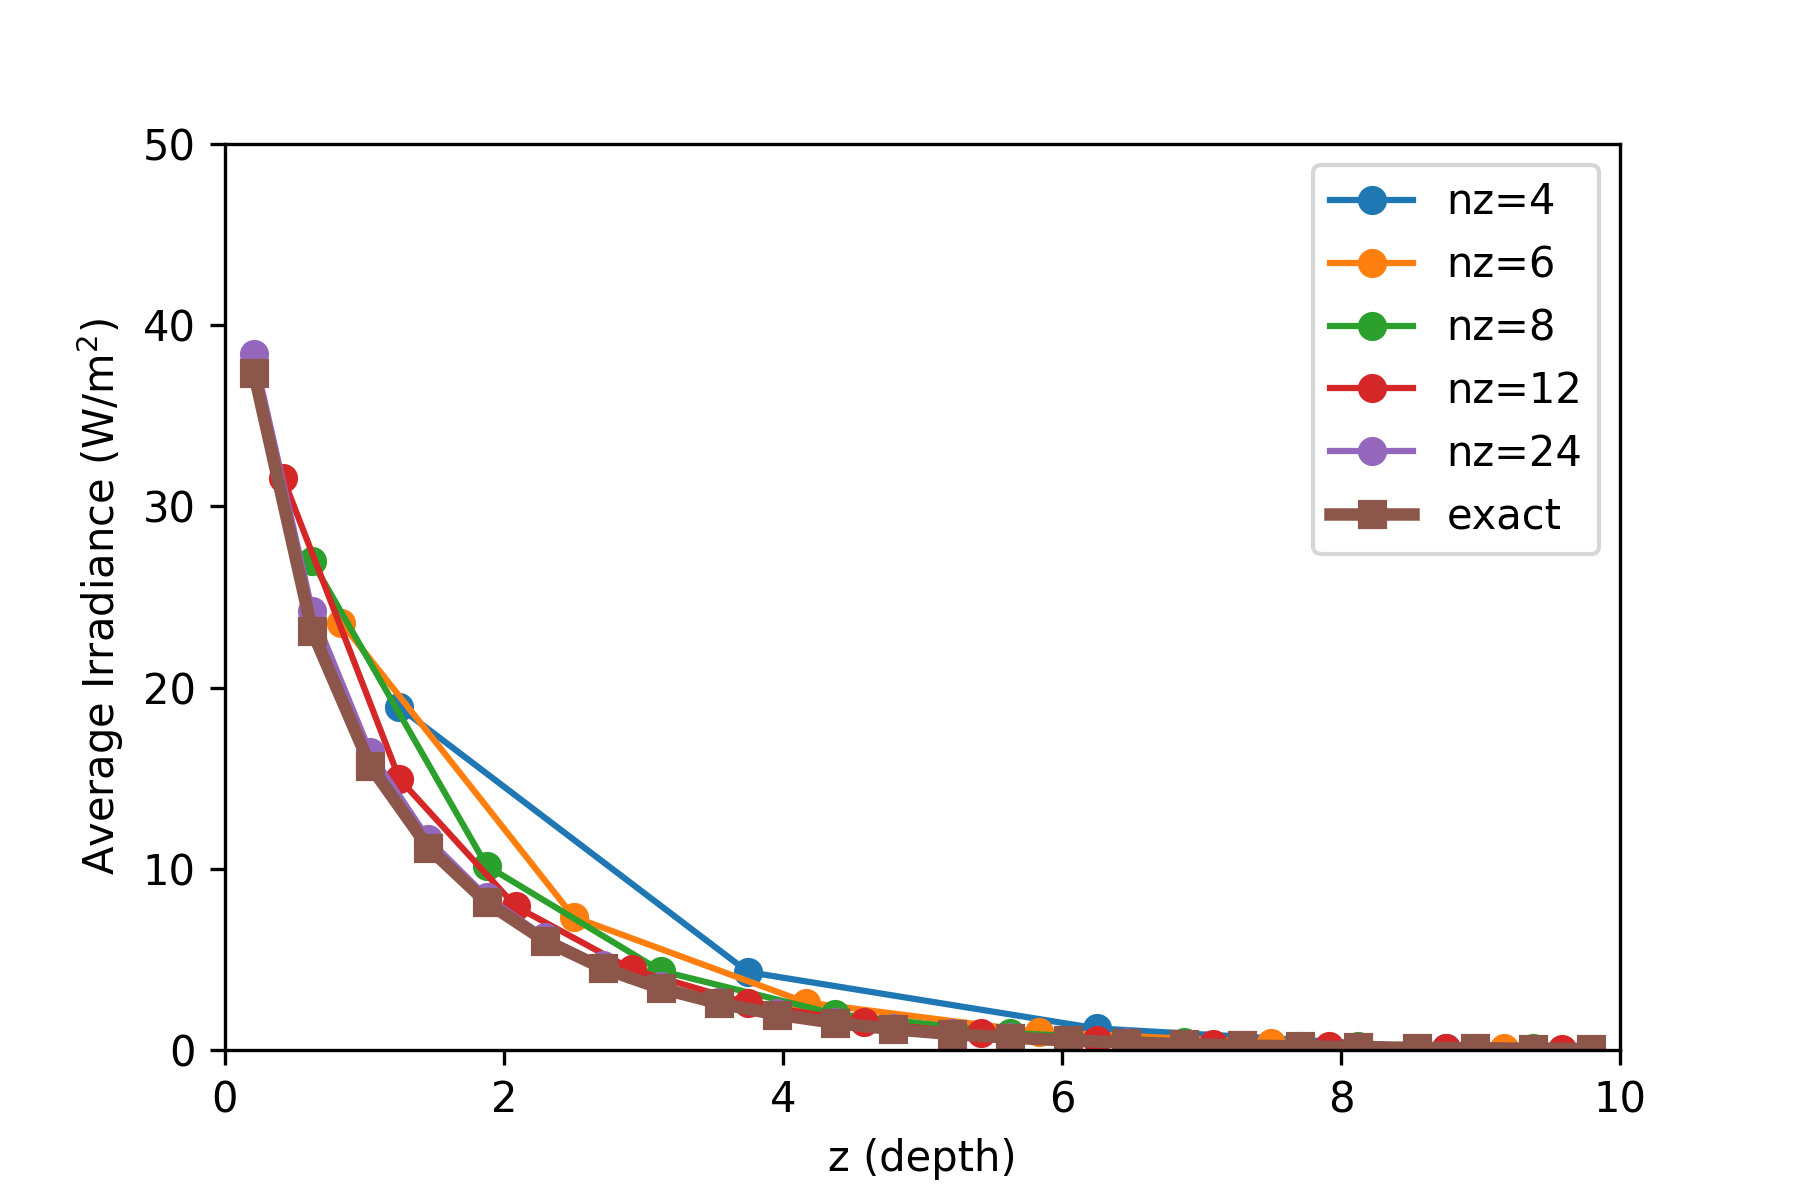
\includegraphics[width=4in]{exact_vs_fd_irrad}
  \caption{Exact v.s. finite difference irradiance, linear scale}
\end{figure}

\begin{figure}[H]
  \centering
  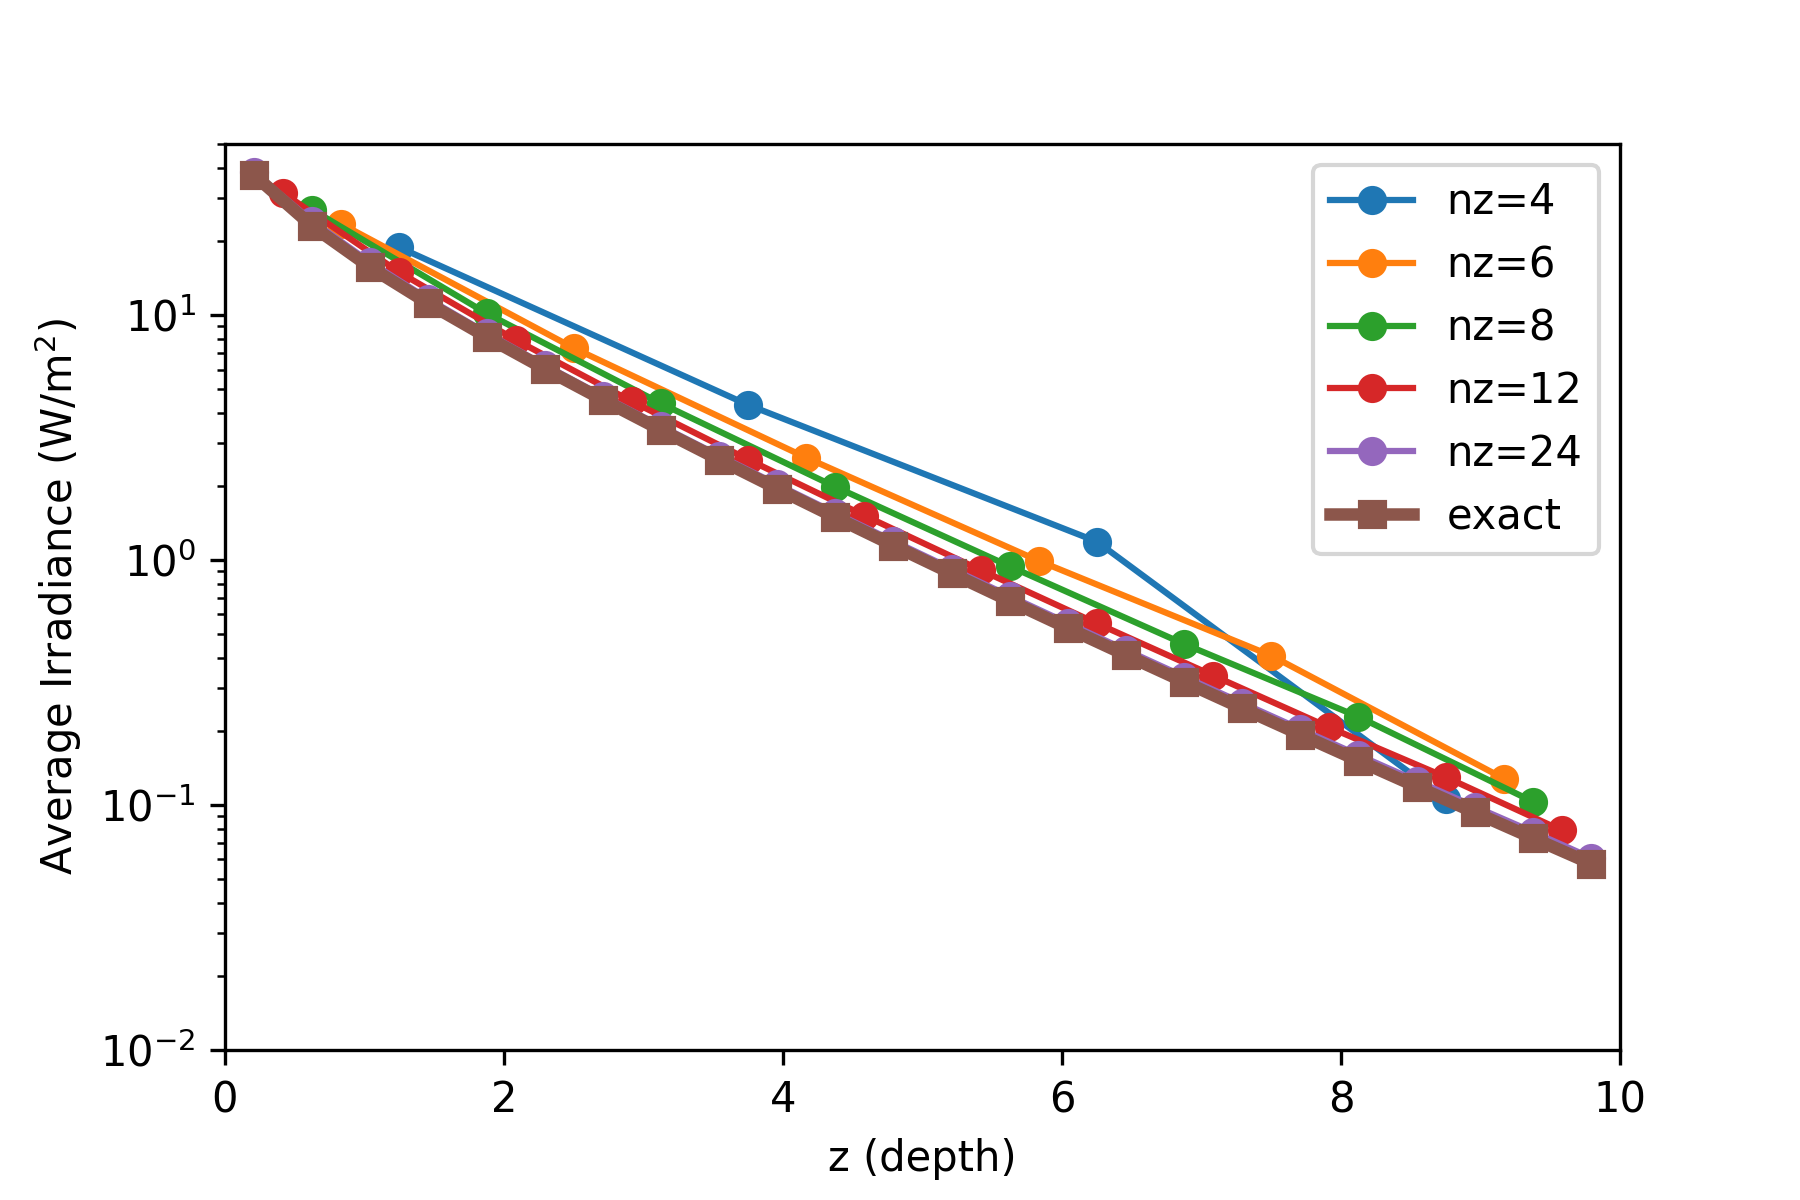
\includegraphics[width=4in]{exact_vs_fd_log_irrad}
  \caption{Exact v.s. finite difference irradiance, log scale}
\end{figure}

\begin{figure}[H]
  \centering
  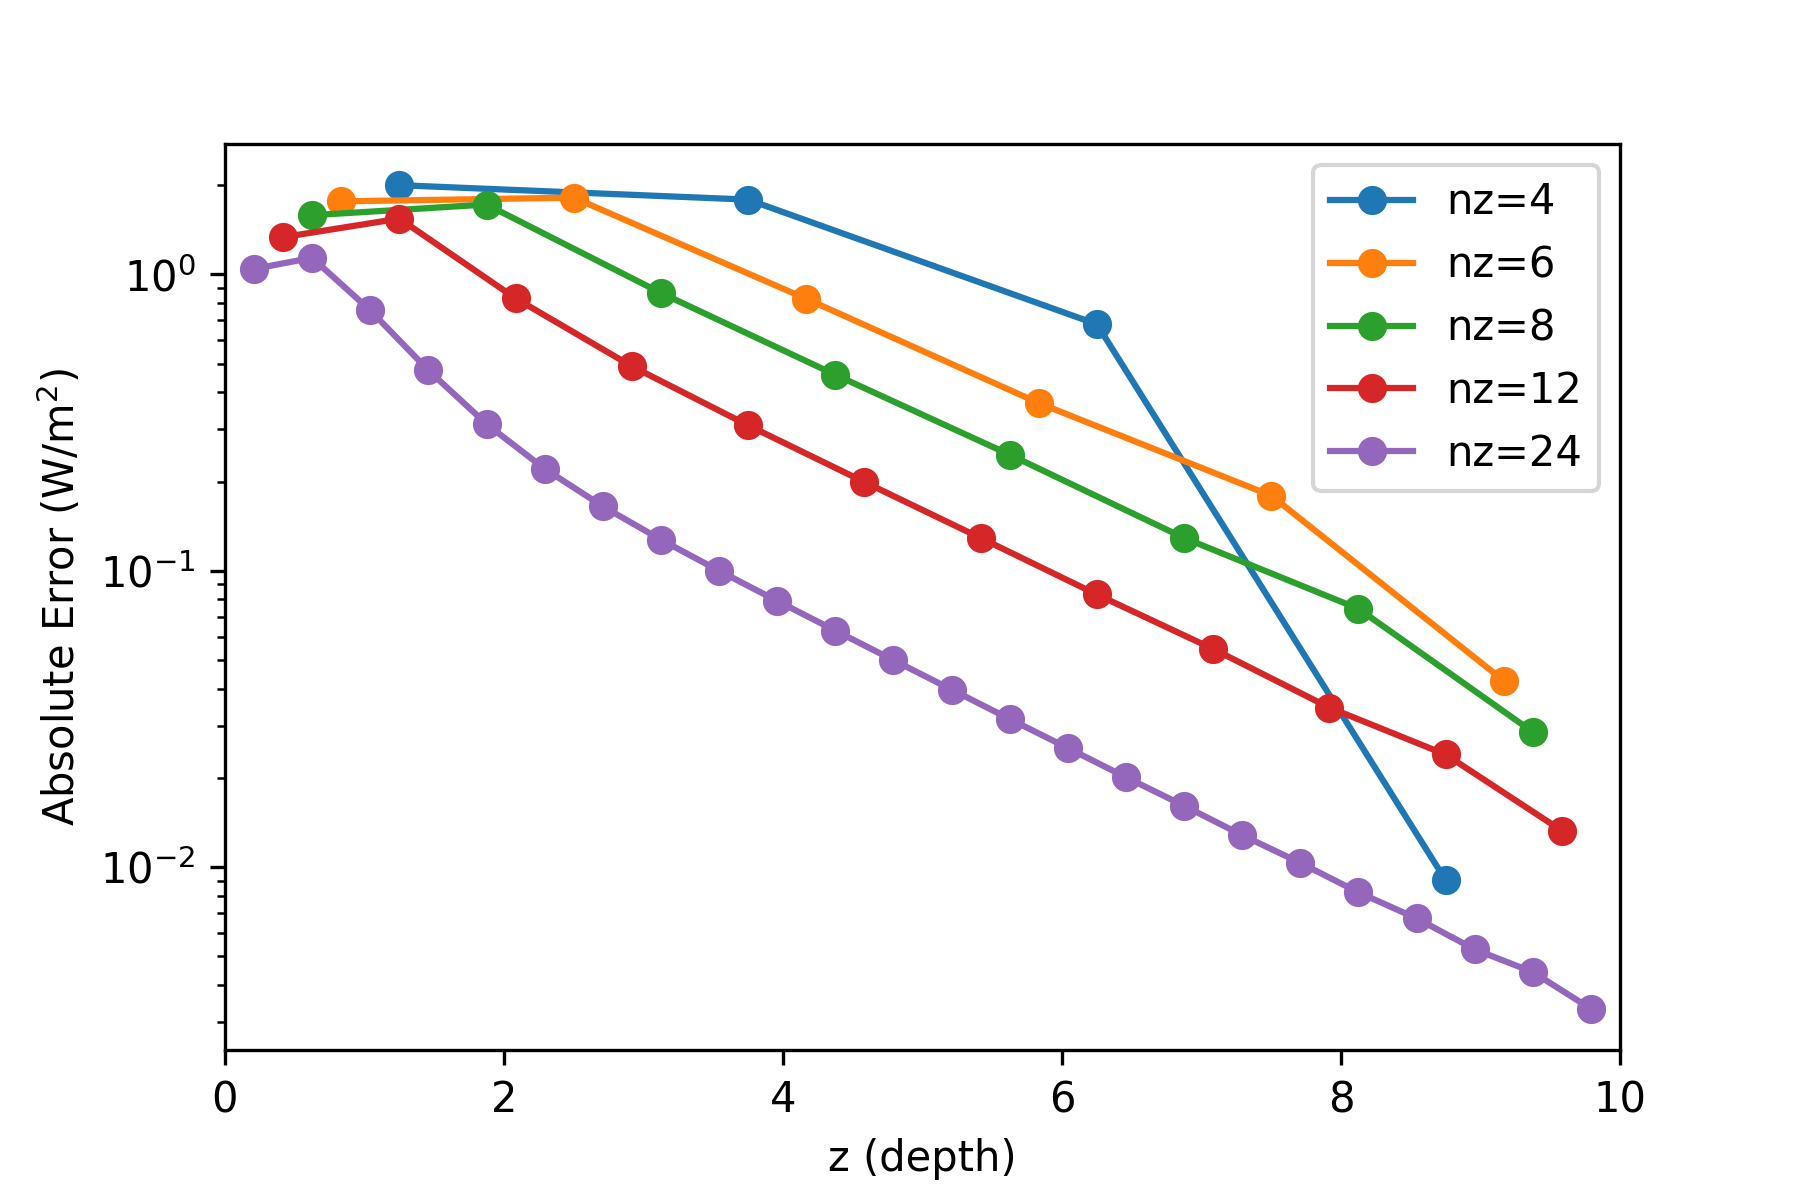
\includegraphics[width=4in]{exact_vs_fd_abs_err}
  \caption{Exact v.s. finite difference irradiance, absolute error}
\end{figure}

\begin{figure}[H]
  \centering
  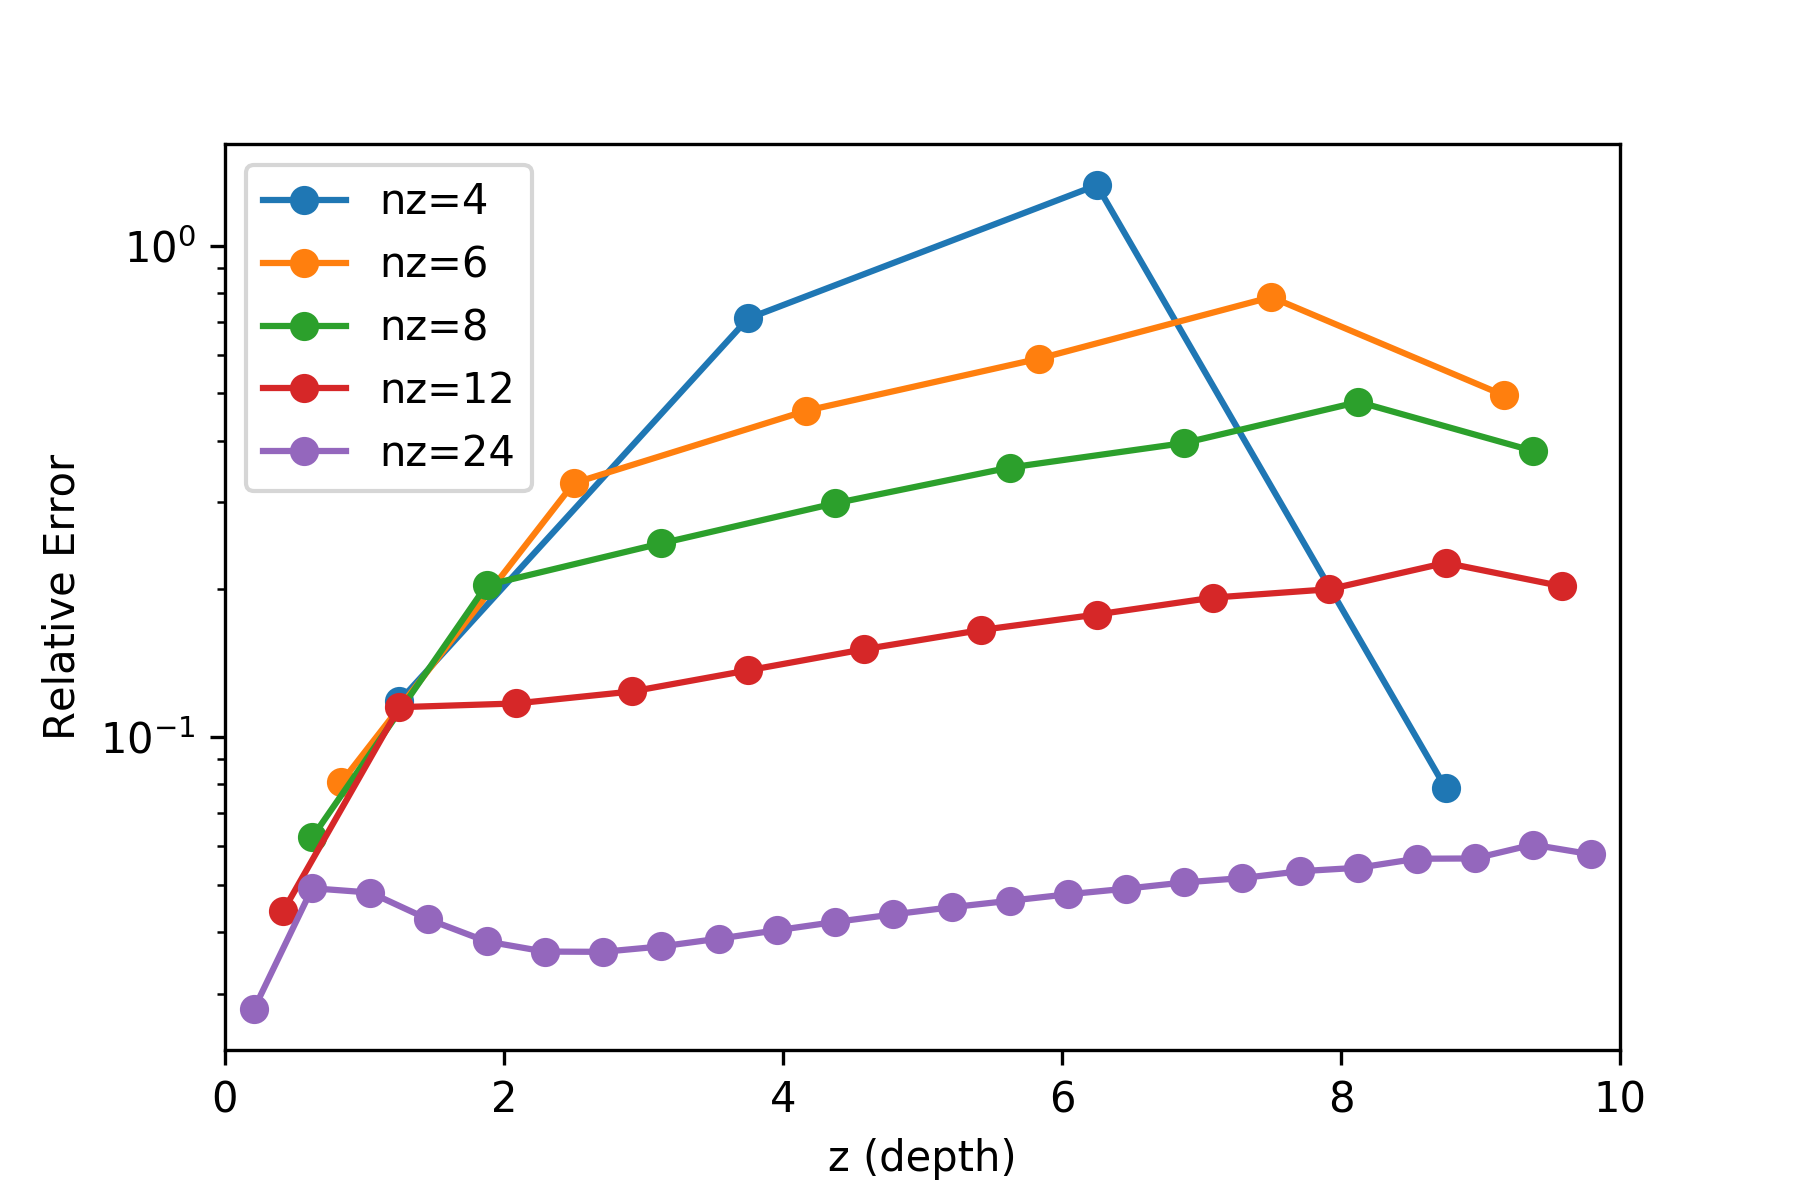
\includegraphics[width=4in]{exact_vs_fd_rel_err}
  \caption{Exact v.s. finite difference irradiance, relative error}
\end{figure}

\begin{figure}[H]
  \centering
  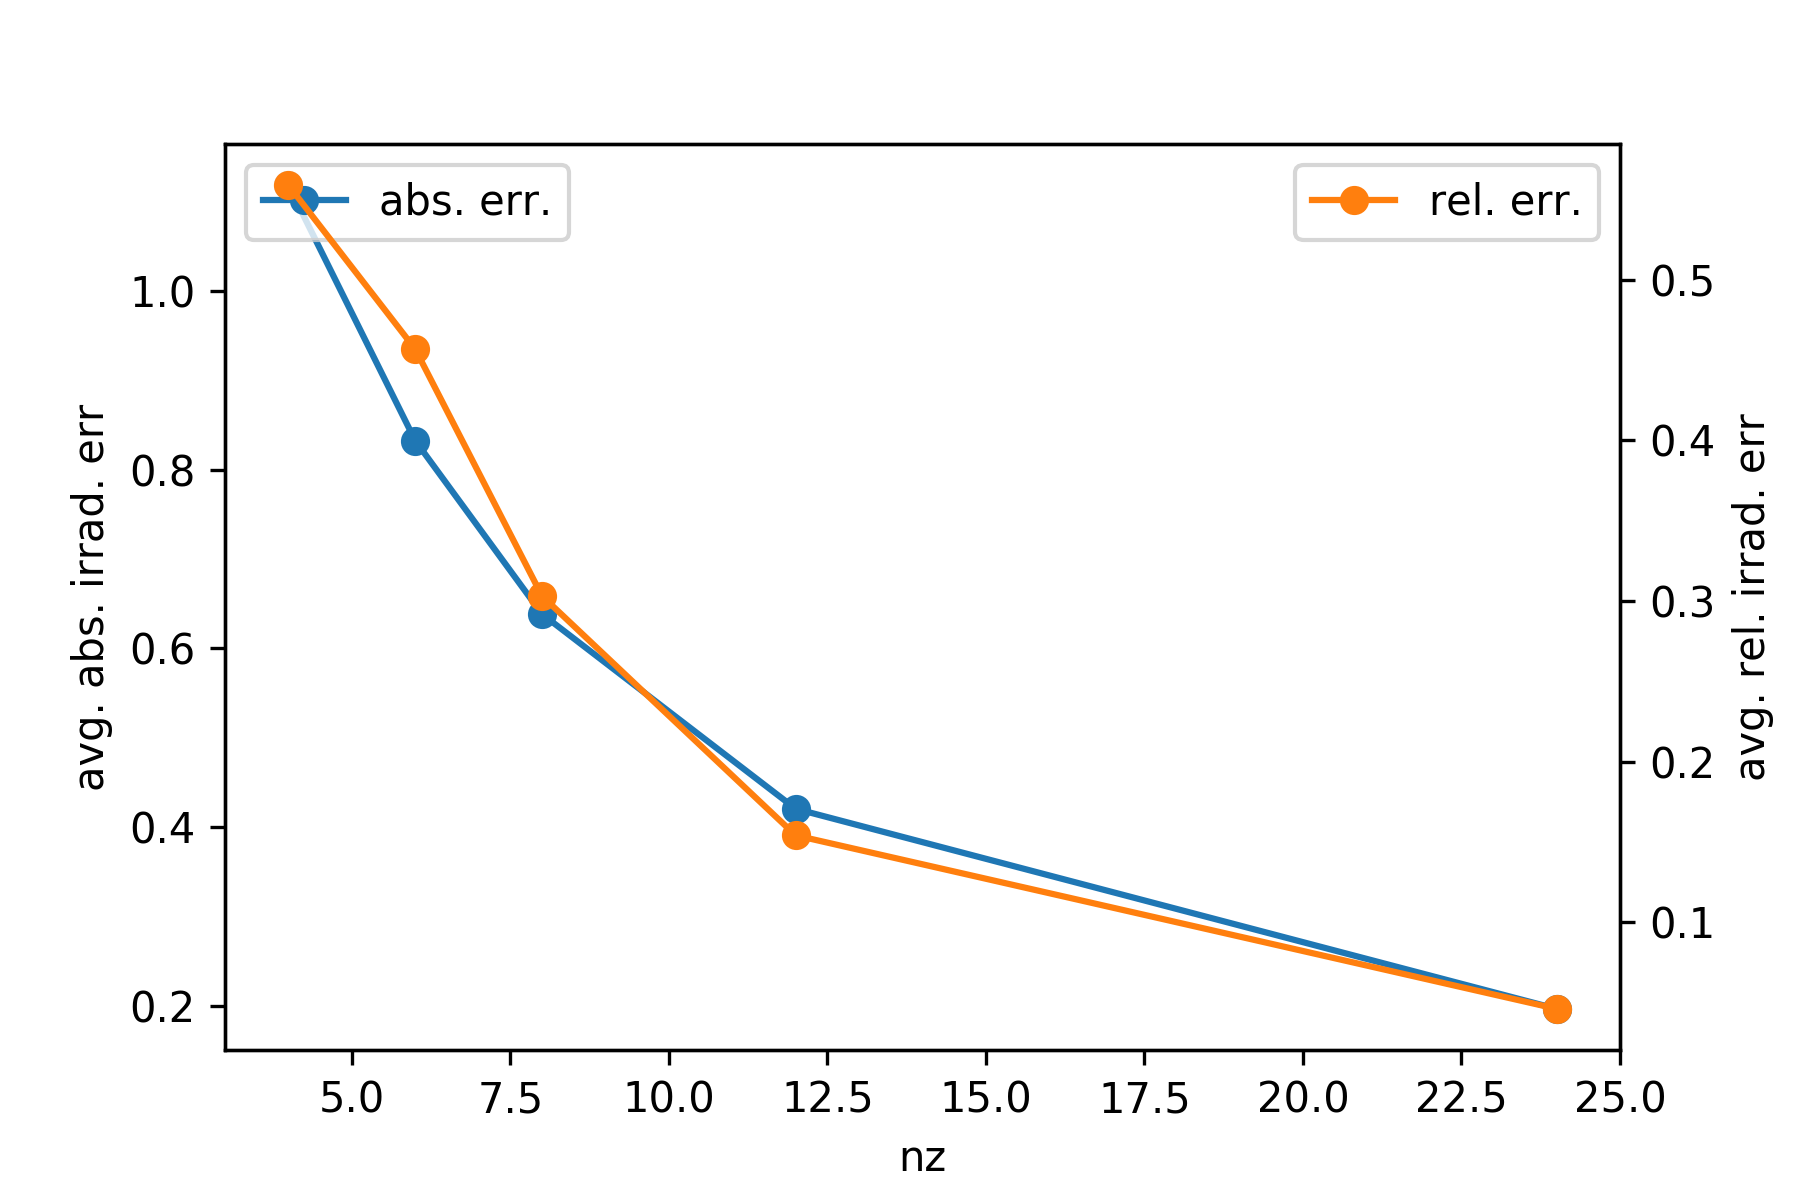
\includegraphics[width=4in]{exact_vs_fd_compare}
  \caption{Exact v.s. finite difference irradiance, relative error v.s. grid resolution}
\end{figure}

\section{Grid Study}
A five dimensional $(x,y,x,\theta,\phi)$ resolution space is nontrivial to characterize.
For the sake of reducing dimensionality, we define generic spatial and angular resolutions
$n_s$ and $n_a$ such that $n_s=n_x=n_y$ and $n_a=n_\theta=n_\phi$.
Remaining is a three-dimensional resolution space, $(n_s,n_z,n_a)$.
Rather than perform calculations at every possible combination of resolutions in the space,
we choose a maximum resolution of $20 \times 20 \times 20$.
We hold two of the three resolutions at the maximum value while varying the third.
For example, Figure \ref{fig:gs_ns} compares $4 \times 20 \times 20$, $6 \times 20 \times 20$, $8 \times 20 \times 20$, etc.
The quantity that we compare is \textit{perceived irradiance}, which is not the simple average irradiance in each depth layer.
Rather, the average is weighted by the normalized spatial kelp distribution to determine the average irradiance experienced by the kelp population.
For more detail, see Section \ref{sec:perceived_irrad}

Note the different natures of convergence in each dimension.
In varying $n_s$, we see that the accuracy is very low for small $n_s$ values.
This is because in these cases, the horizontal grid cells are too large to capture any detail
about the kelp fronds near the bottom where they are very small.
The kelp is effectively not present in these layers, and therefore the perceived irradiance is zero.
After increasing the resolution past this minimum threshold, however, little improvement results
from increasing $n_s$ further, as seen in Figure \ref{fig:gs_ns}.
On the other hand, Figure \ref{fig:gs_nz} shows that increasing the vertical resolution
consistently improves the accuracy of the solution.
Figure \ref{fig:gs_na} shows that $n_a$ is somewhere between the two,
demonstrating clear improvement with increasing resolution, though the improvement is not uniform over depth.
Figure \ref{fig:gs_compare} shows the trend of increasing accuracy with increasing resolution in each dimension.

\begin{figure}[H]
  \centering
  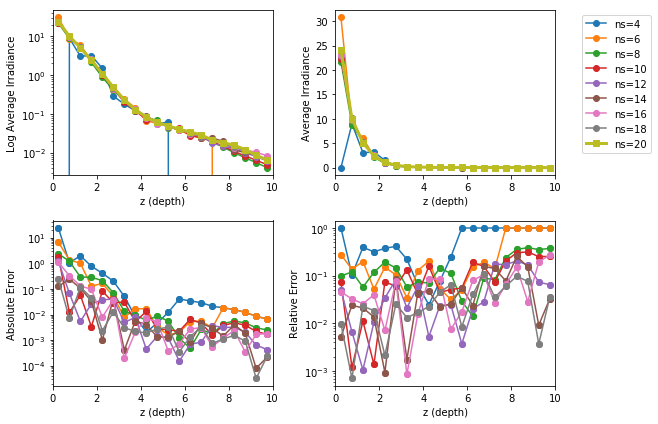
\includegraphics[width=5in]{gs_ns_20}
  \caption{Grid study, $n_s$}
  \label{fig:gs_ns}
\end{figure}

\begin{figure}[H]
  \centering
  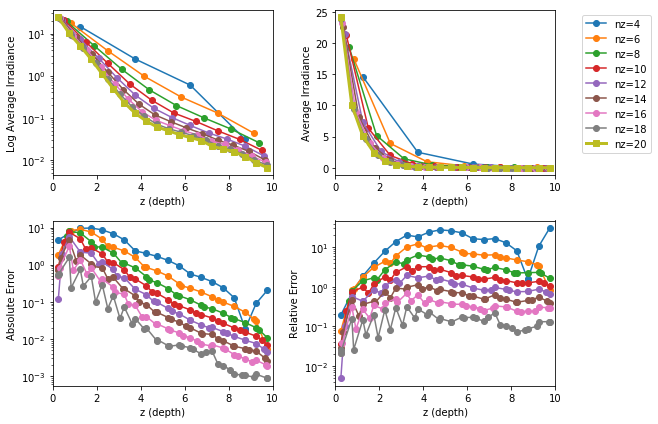
\includegraphics[width=5in]{gs_nz_20}
  \caption{Grid study, $n_z$}
  \label{fig:gs_nz}
\end{figure}

\begin{figure}[H]
  \centering
  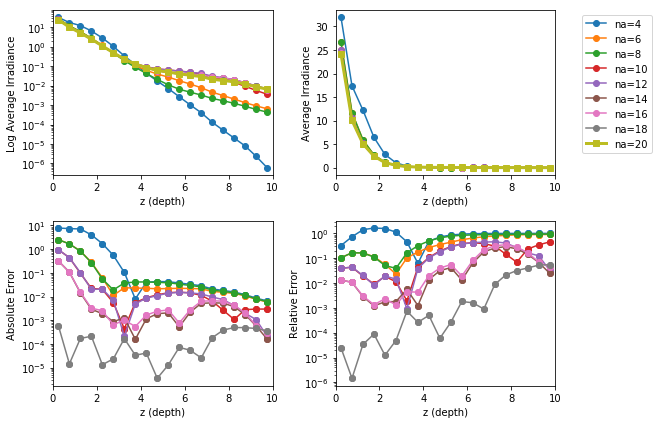
\includegraphics[width=5in]{gs_na_20}
  \caption{Grid study, $n_a$}
  \label{fig:gs_na}
\end{figure}

\begin{figure}[H]
  \centering
  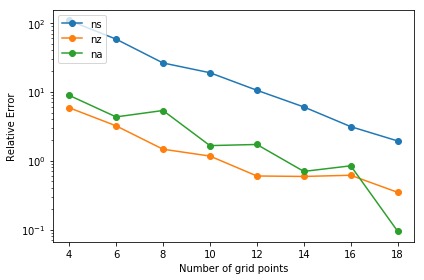
\includegraphics[width=5in]{gs_20}
  \caption{Grid study, summary}
  \label{fig:gs_compare}
\end{figure}


\section{Asymptotic Convergence}
\label{sec:asym_conv}

In this section, the four water cases from Table \ref{tab:petzold} are considered.
In each case, the full finite difference solution is calculated on an $18 \times 18 \times 18$ grid,
and asymptotic approximations are given, varying the number of terms used in the asymptotic series.
Perceived irradiances are shown, as well as errors from the finite difference solution.

In the first two cases, when the scattering coefficient is the same order or smaller as the absorption coefficient,
the asymptotic approximation converges to the finite difference solution.
However, in the very turbid water of the San Diego Harbor, the scattering coefficient is an order of magnitude higher
than the absorption coefficient, causing the asymptotic solution to quickly diverge.
In figure \ref{fig:asym_conv_compare}, average relative errors for the two converging cases are shown.
In both cases, the accuracy improves with more scattering events until it plateaus.
In the first case, 4 scattering events is sufficient, whereas in the second, the accuracy improves until 12 scattering events.

\begin{figure}[H]
  \centering
  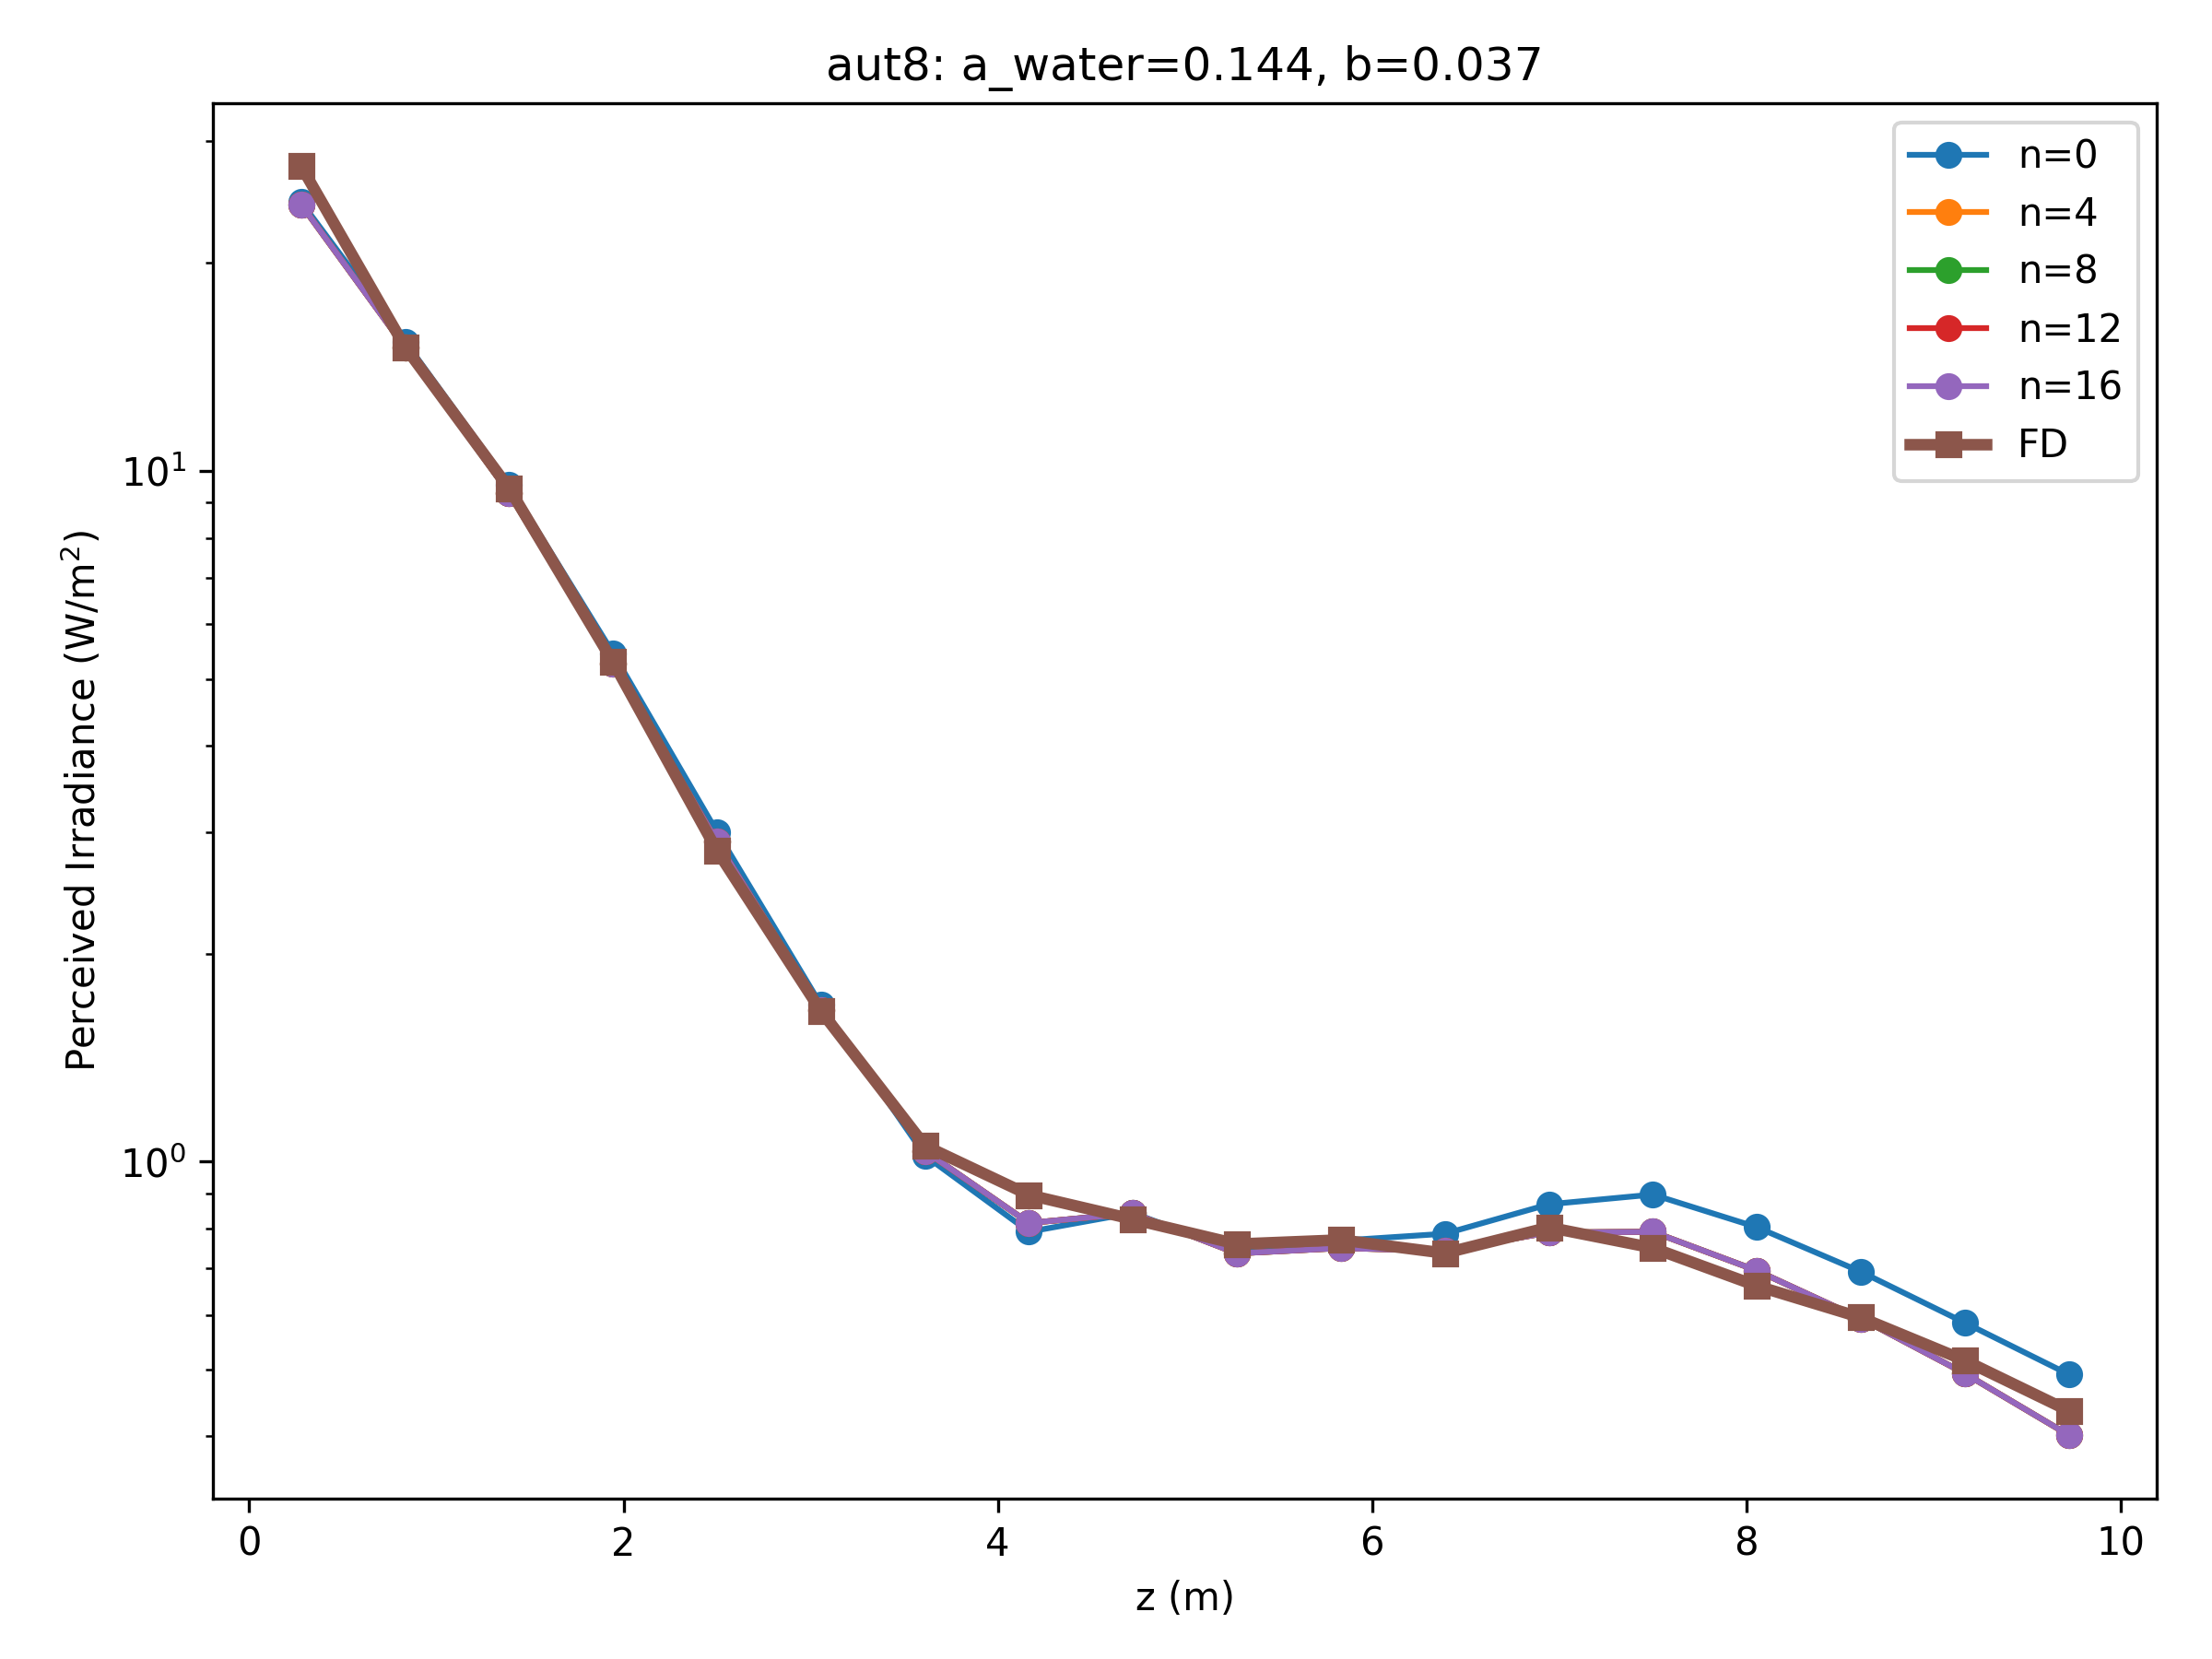
\includegraphics[width=4in]{asym_conv_irrad_aut8}
  \caption{Successive asymptotic approximations, irradiance: \texttt{AUT8}}
\end{figure}

\begin{figure}[H]
  \centering
  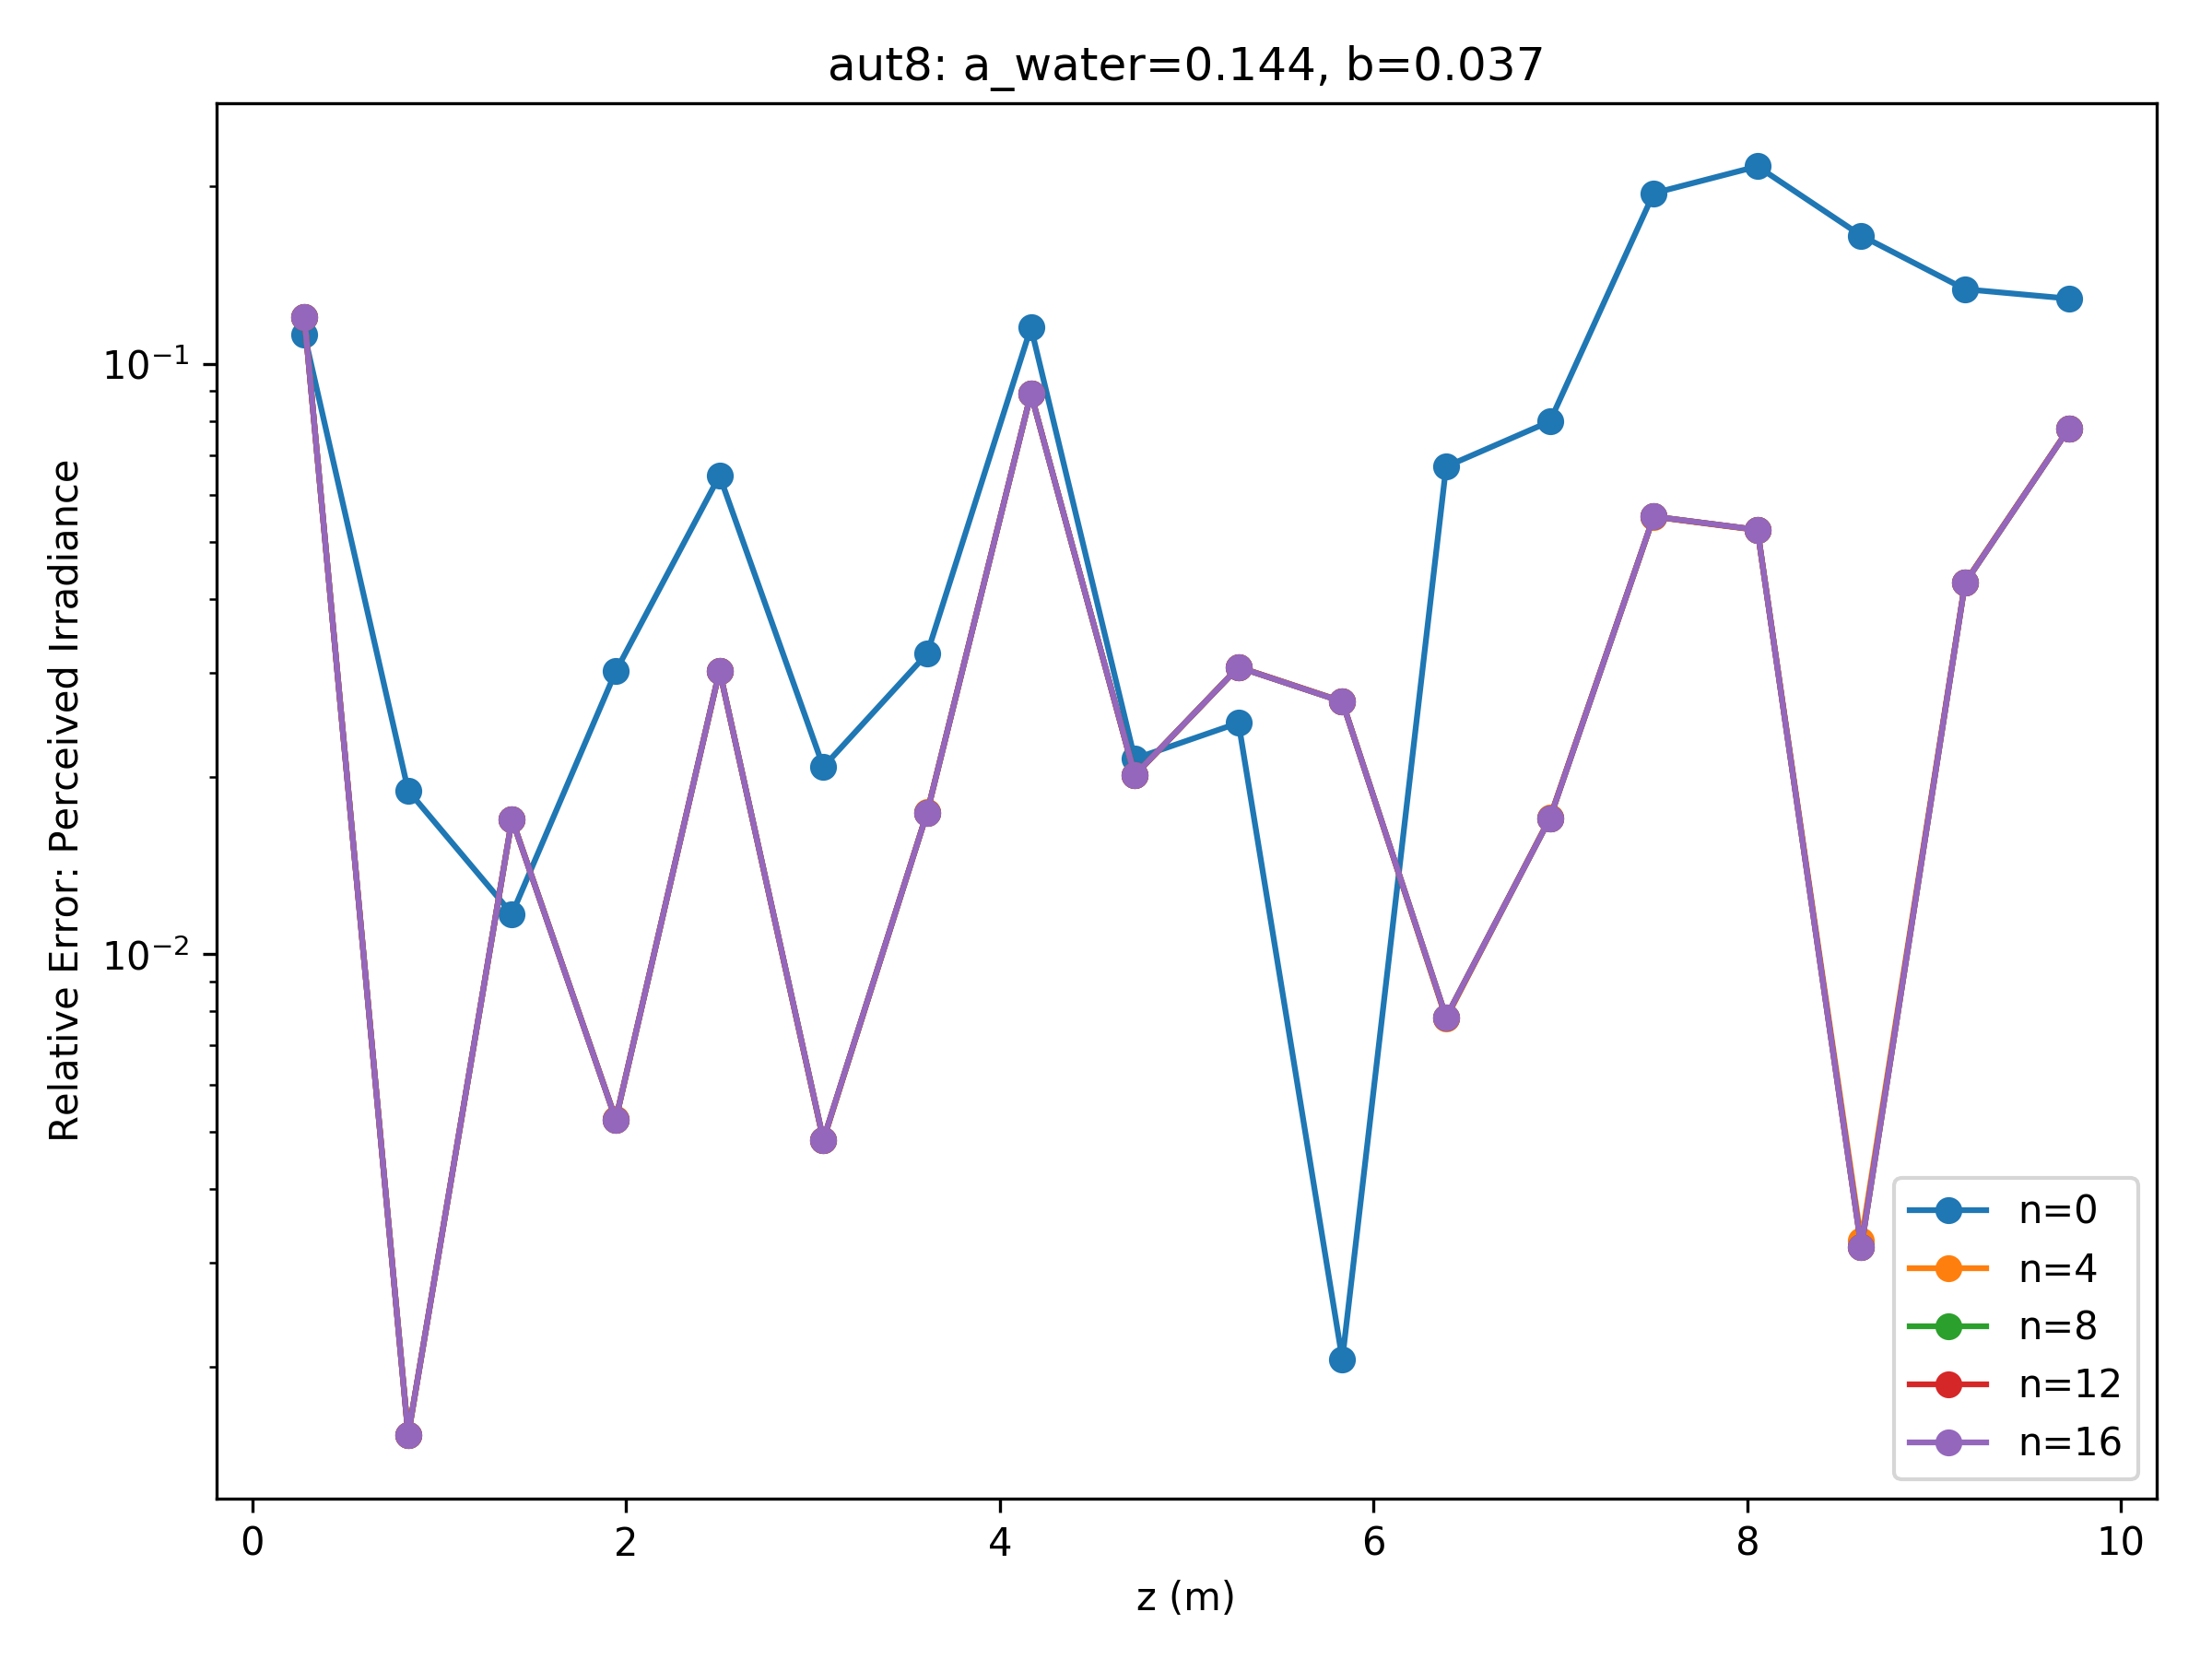
\includegraphics[width=4in]{asym_conv_rel_err_aut8}
  \caption{Successive asymptotic approximations, relative error: \texttt{AUT8}}
\end{figure}


\begin{figure}[H]
  \centering
  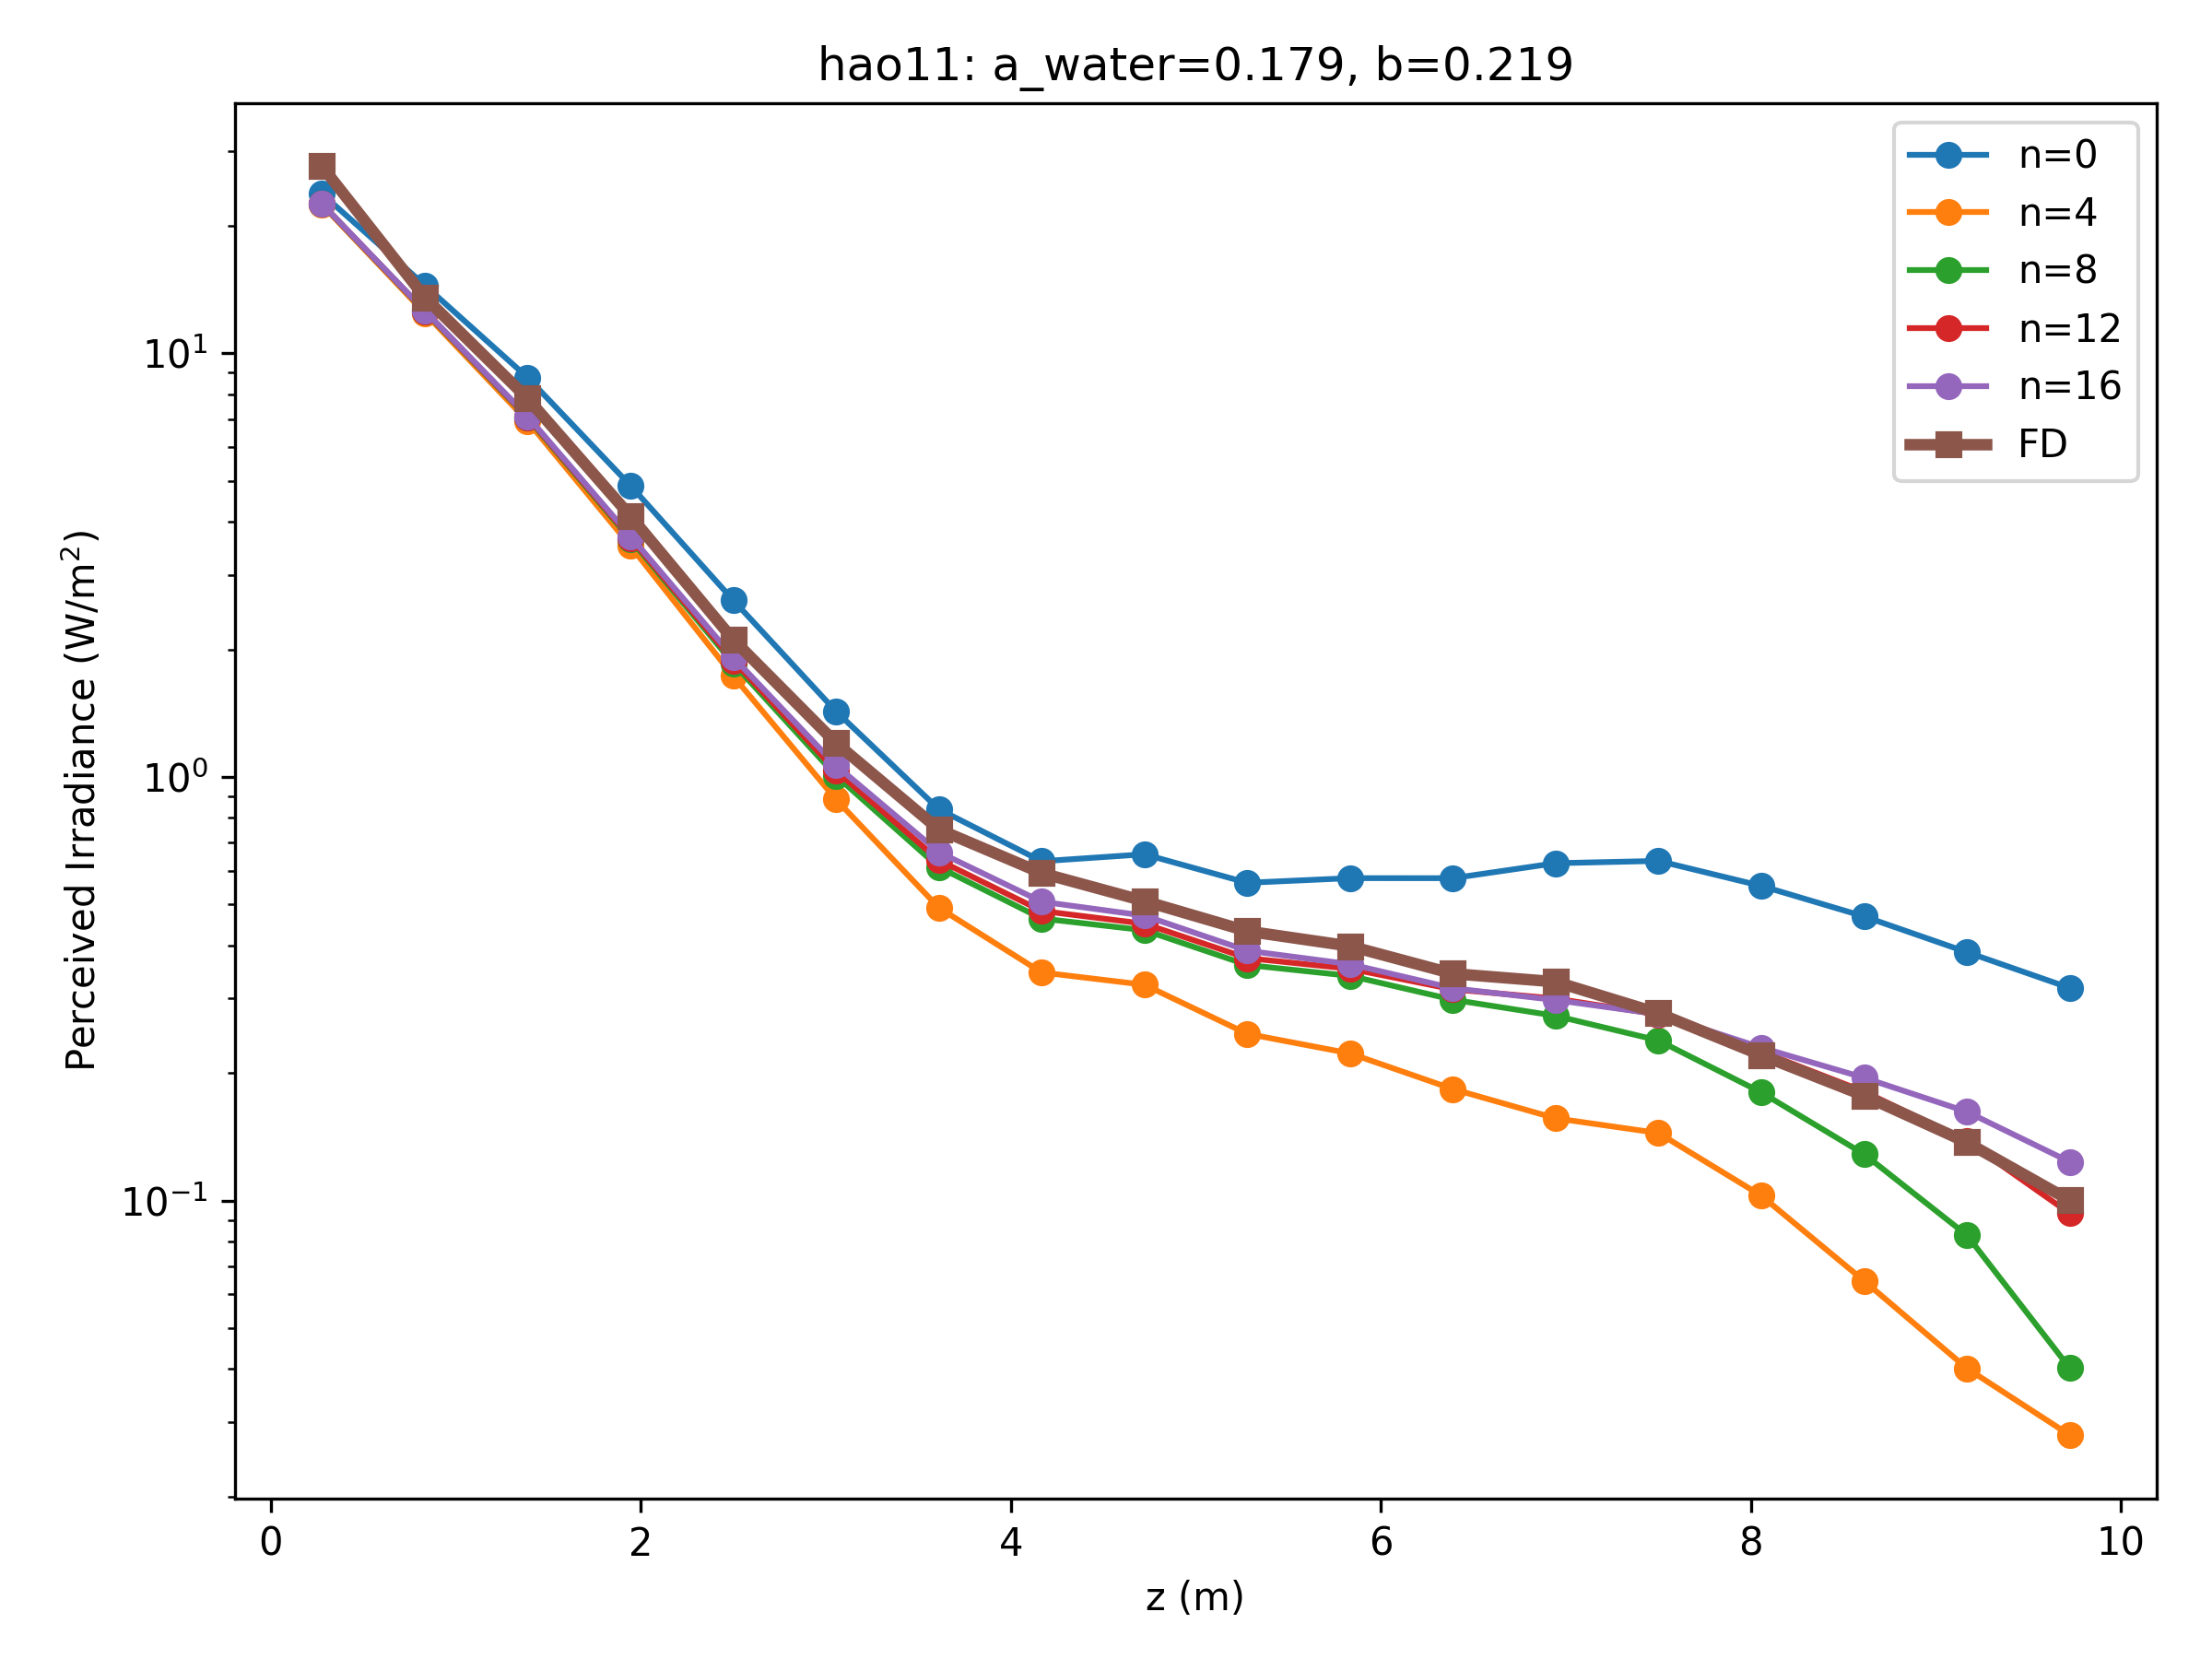
\includegraphics[width=4in]{asym_conv_irrad_hao11}
  \caption{Successive asymptotic approximations, irradiance: \texttt{HAO11}}
\end{figure}

\begin{figure}[H]
  \centering
  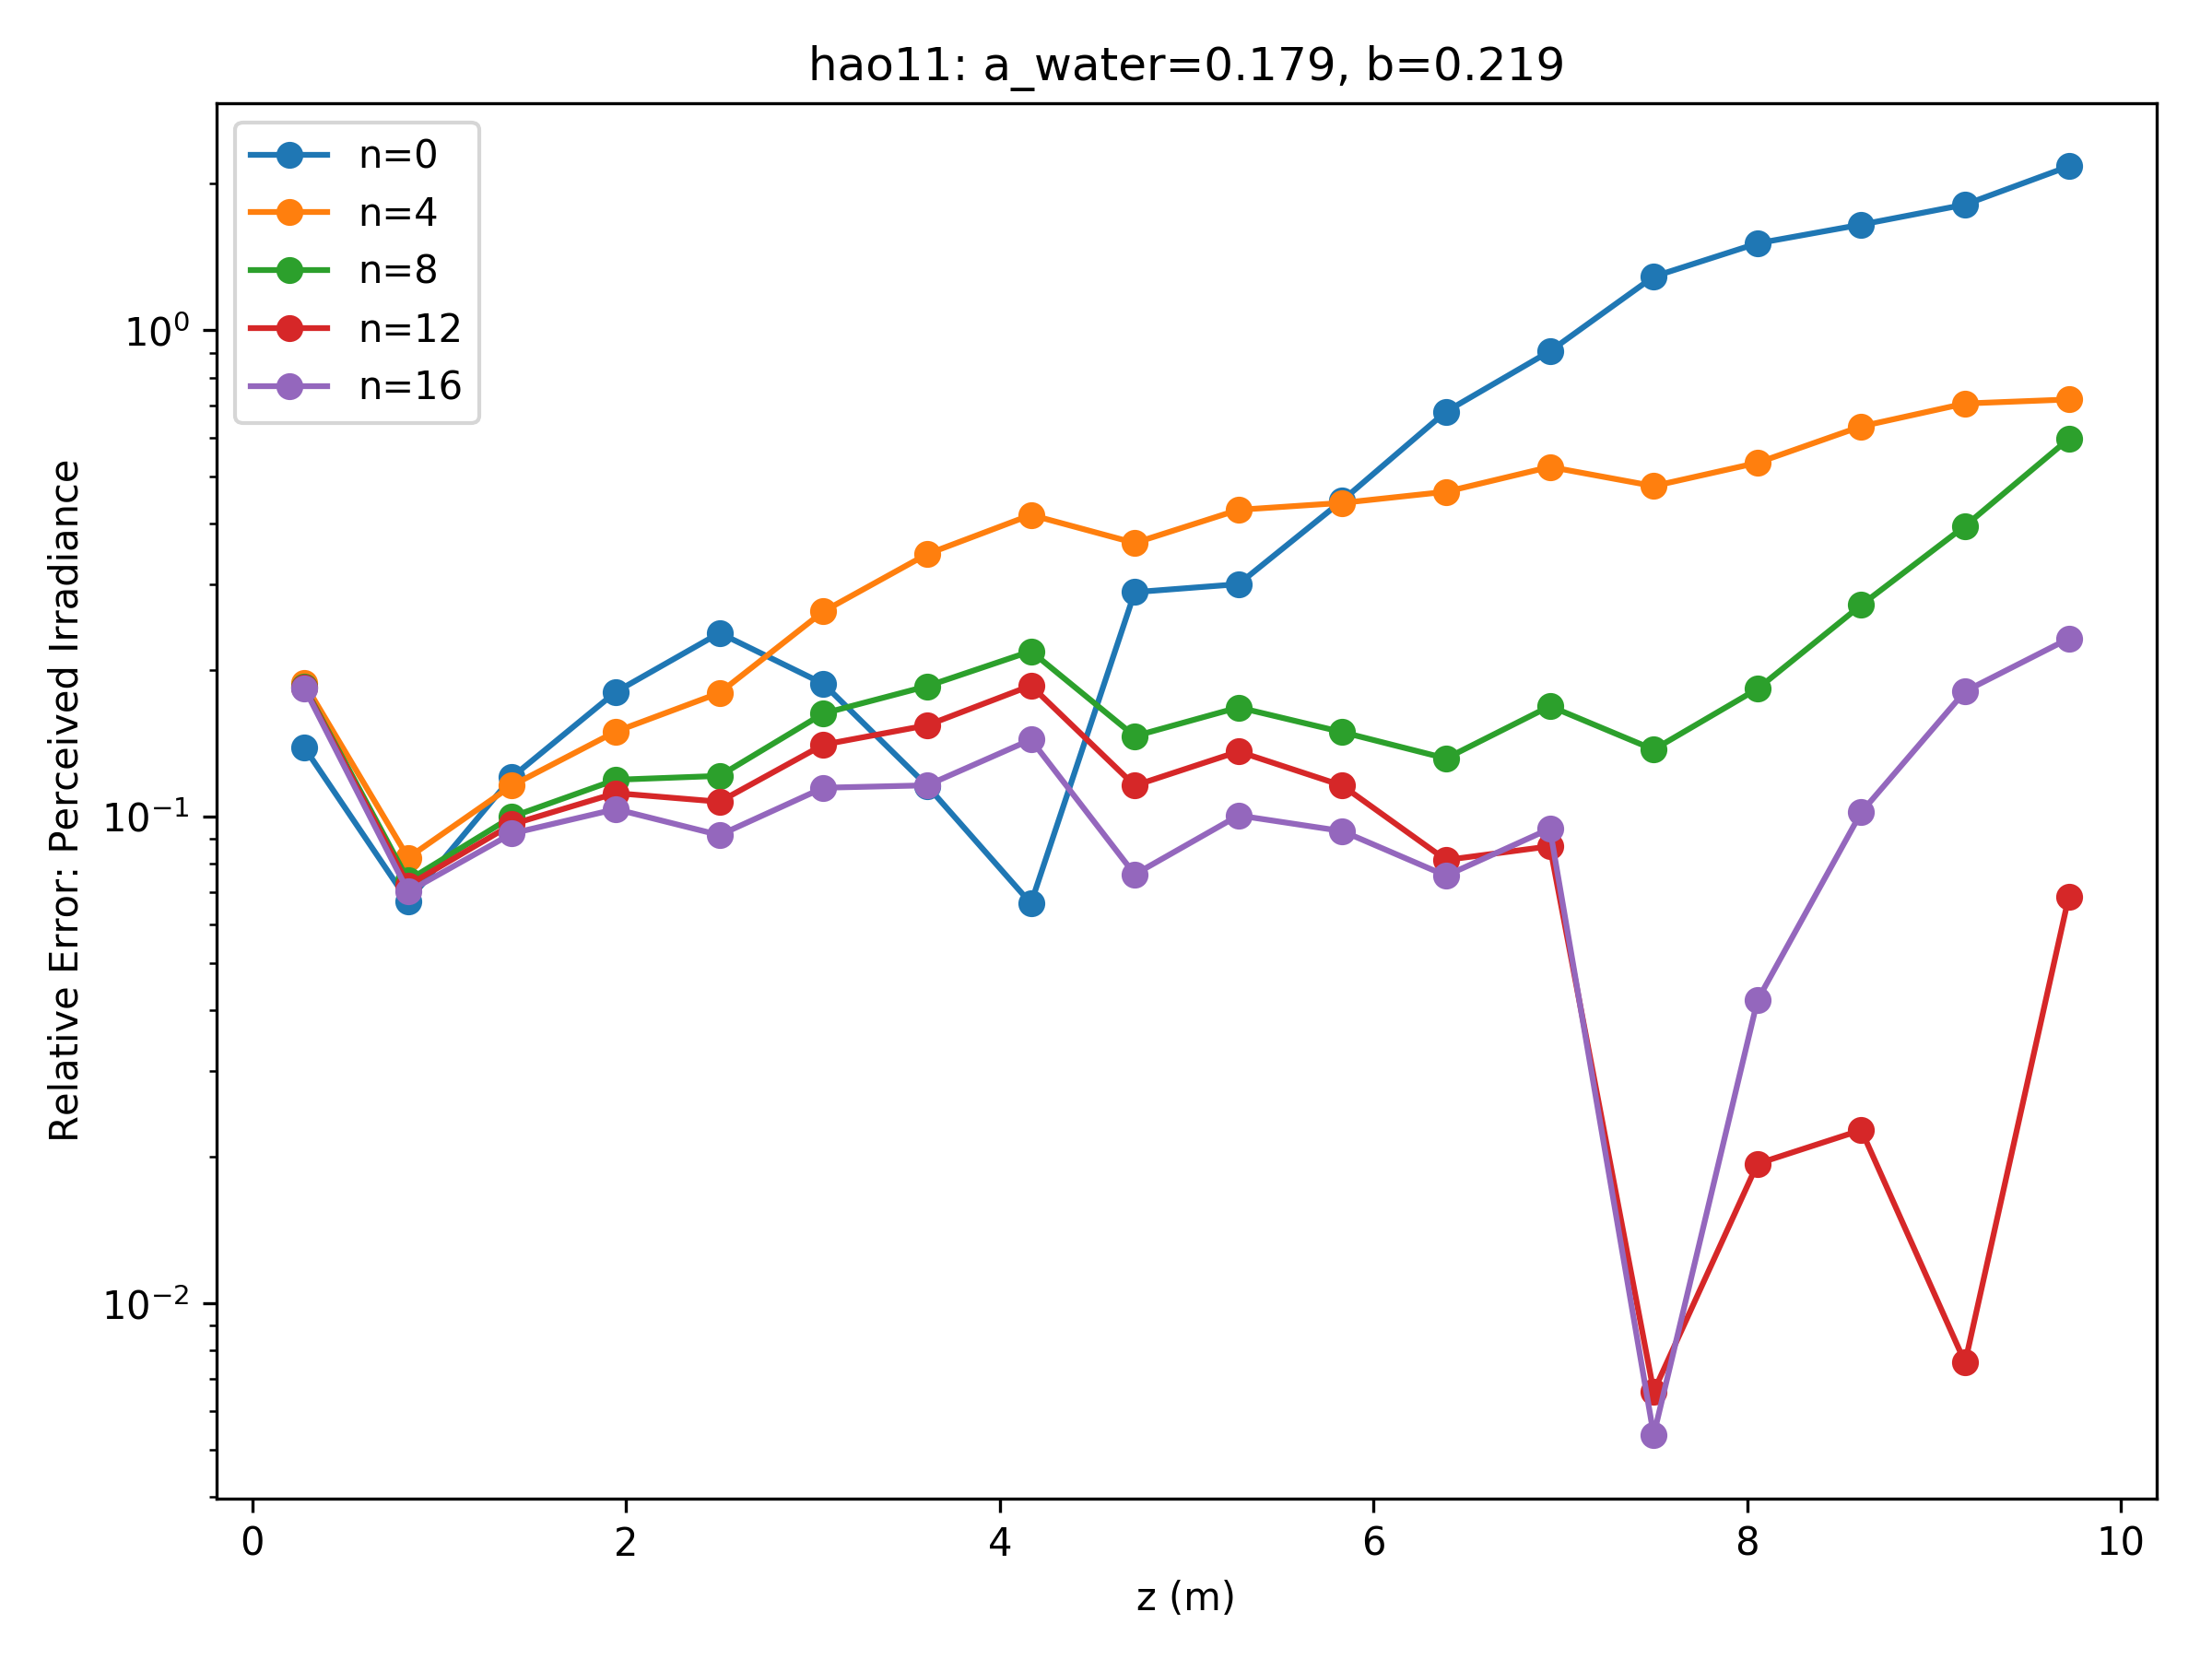
\includegraphics[width=4in]{asym_conv_rel_err_hao11}
  \caption{Successive asymptotic approximations, relative error: \texttt{HAO11}}
\end{figure}


\begin{figure}[H]
  \centering
  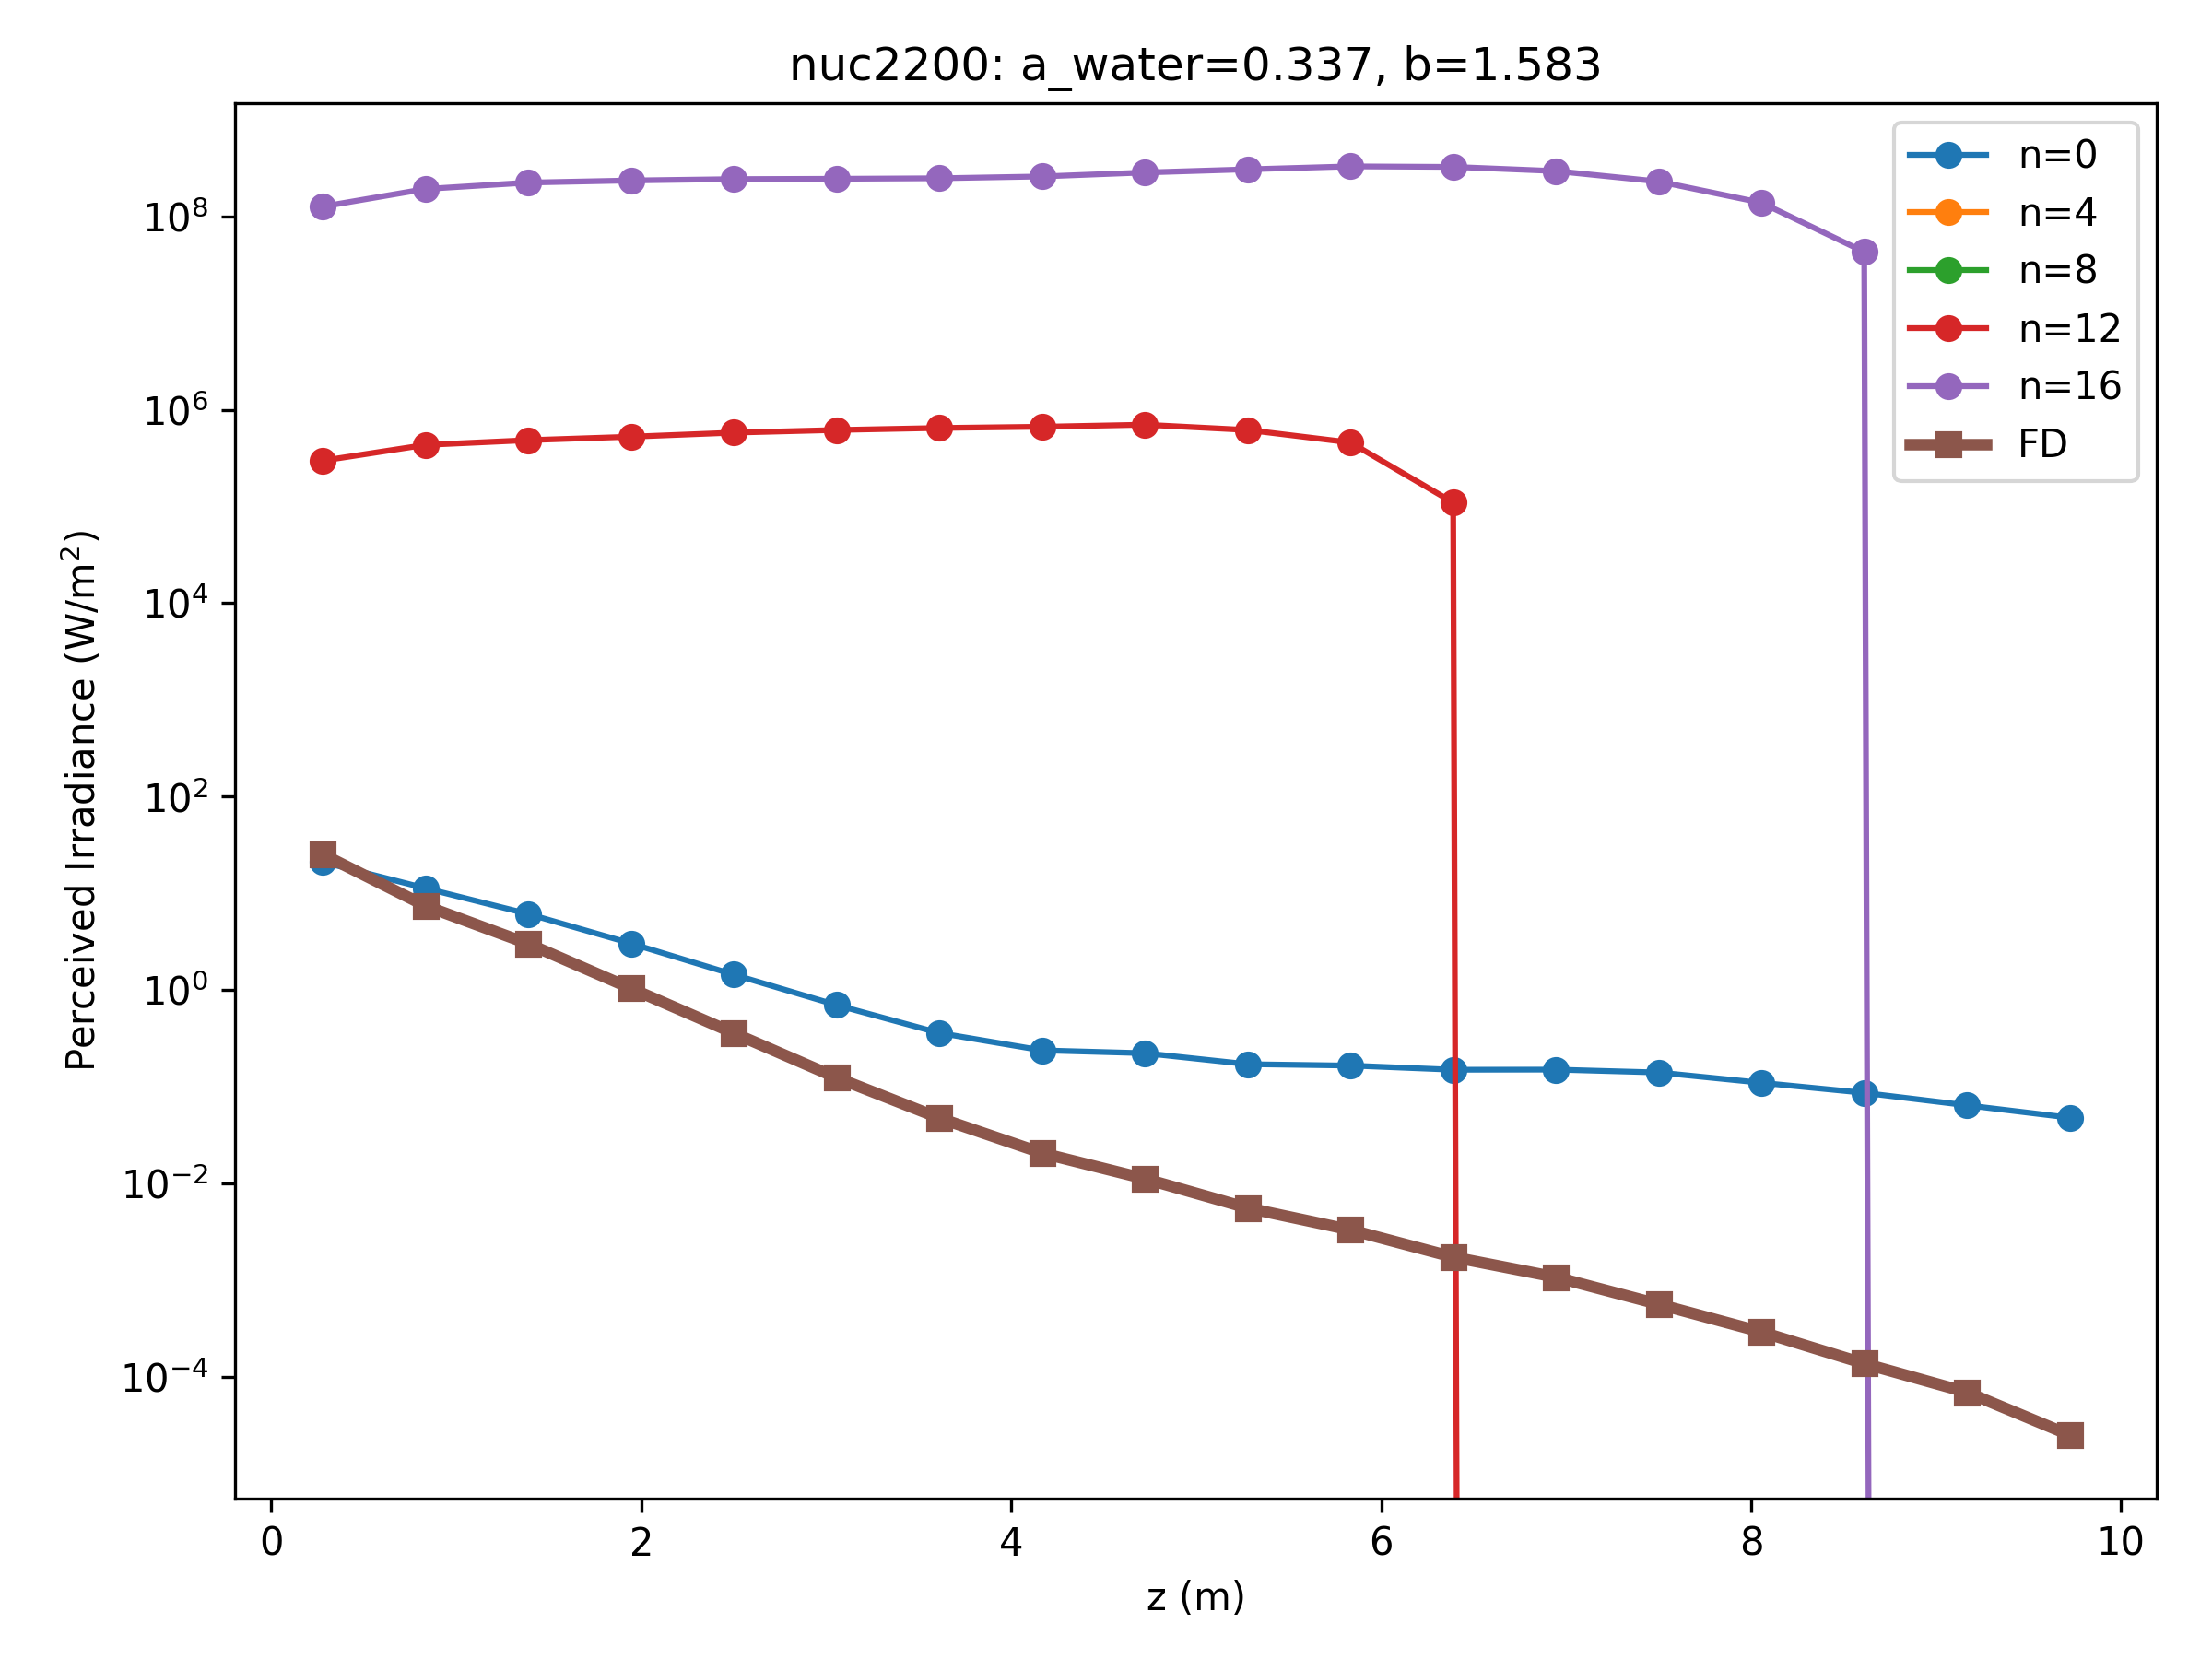
\includegraphics[width=4in]{asym_conv_irrad_nuc2200}
  \caption{Successive asymptotic approximations, irradiance: \texttt{NUC2200}}
\end{figure}

\begin{figure}[H]
  \centering
  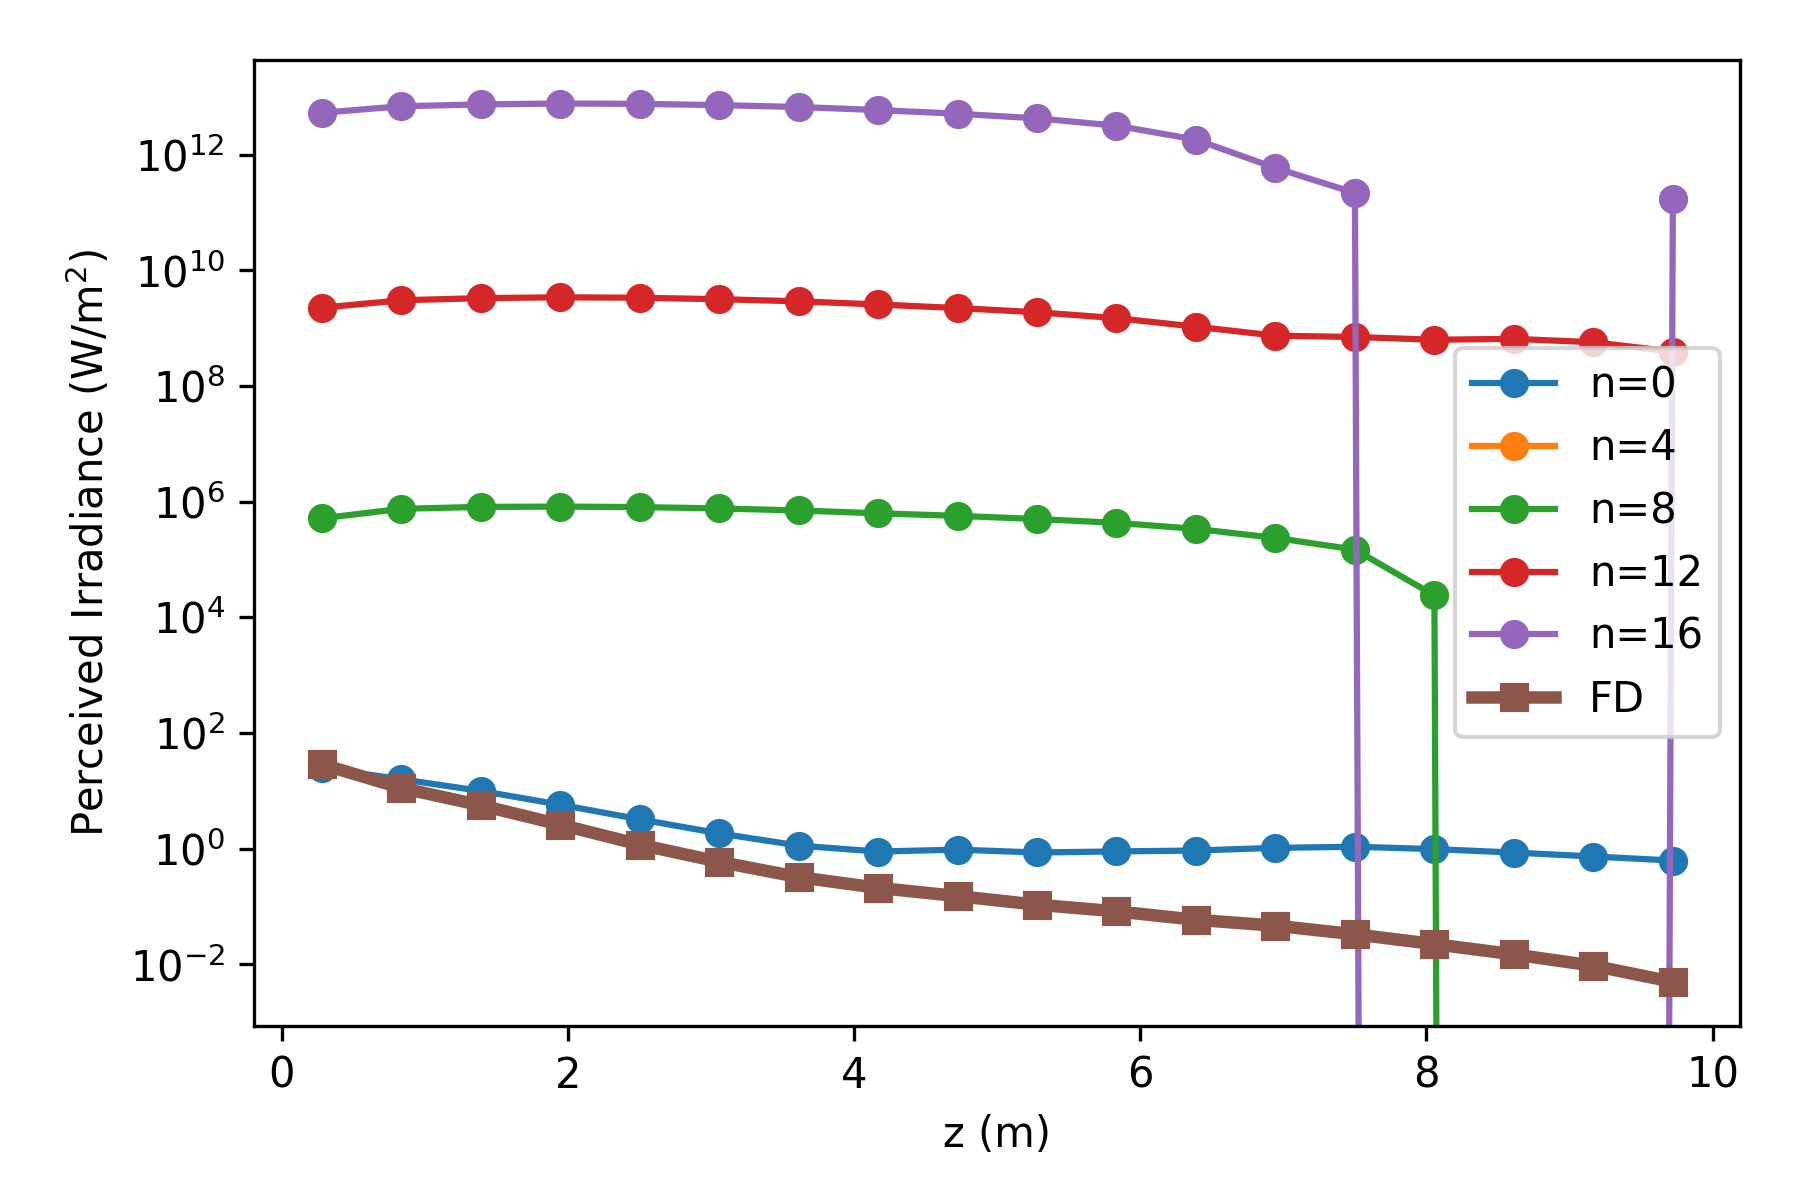
\includegraphics[width=4in]{asym_conv_irrad_nuc2240}
  \caption{Successive asymptotic approximations, relative error: \texttt{NUC2240}}
\end{figure}


\begin{figure}[H]
  \centering
  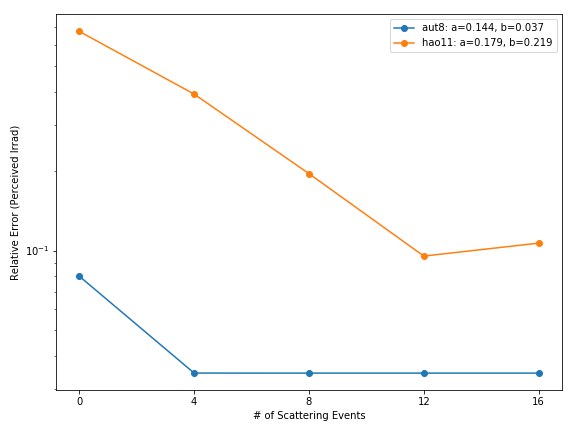
\includegraphics[width=4in]{asym_conv_compare}
  \caption{Comparison of asymptotic approximations for various waters.}
  \label{fig:asym_conv_compare}
\end{figure}

\section{Sensitivity Analysis}
In this section, we demonstrate the effect of varying some of the parameters of the model.
The 12-term asymptotic approximation is used.
In Figure \ref{fig:sens_analysis_a_water} and Figure \ref{fig:sens_analysis_b}, the solution
is shown to diverge when the ratio $b/a$ is too large, as in Section \ref{sec:asym_conv}.

\begin{figure}[H]
  \centering
  \vspace{-3em}
  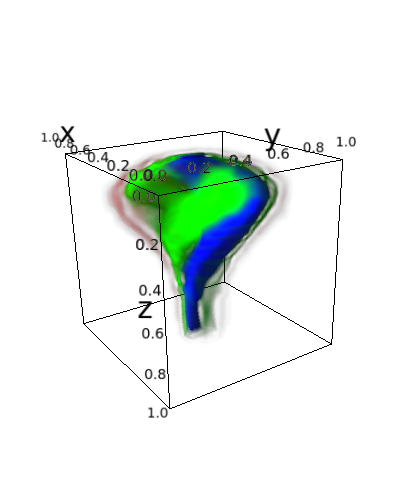
\includegraphics[width=0.45\textwidth]{top-heavy_kelp}
  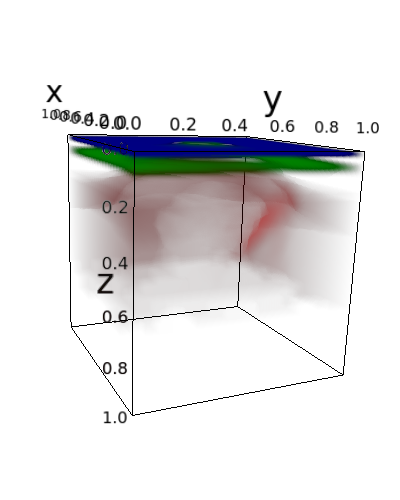
\includegraphics[width=0.45\textwidth]{top-heavy_irrad}
  \caption{\textit{top-heavy} kelp distribution (left) and no-scattering irradiance profile (right)}
\end{figure}

\begin{figure}[H]
  \centering
  \vspace{-3em}
  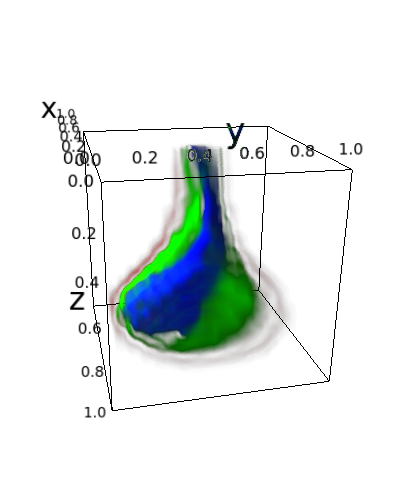
\includegraphics[width=0.45\textwidth]{bottom-heavy_kelp}
  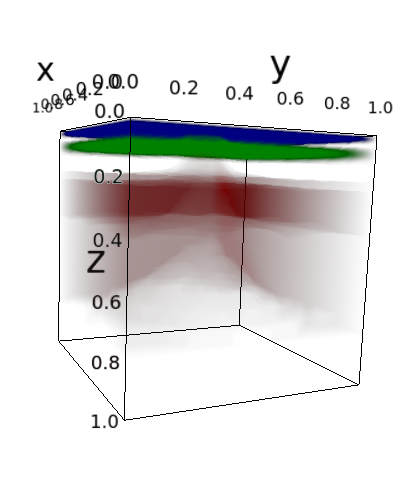
\includegraphics[width=0.45\textwidth]{bottom-heavy_irrad}
  \caption{\textit{bottom-heavy} kelp distribution (left) and no-scattering irradiance profile (right)}
\end{figure}

\begin{figure}[H]
  \centering
  \vspace{-3em}
  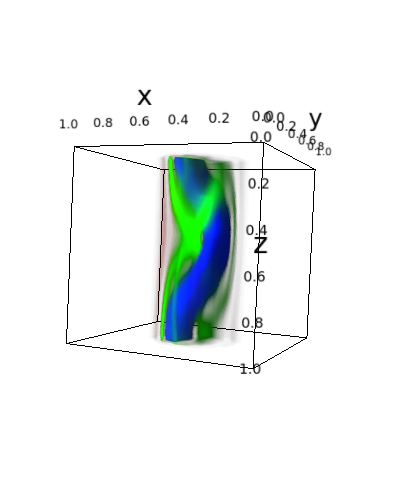
\includegraphics[width=0.45\textwidth]{uniform_kelp}
  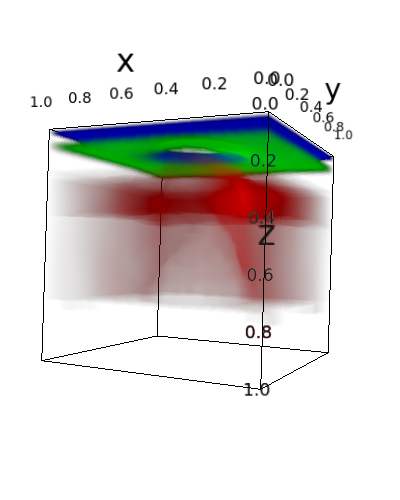
\includegraphics[width=0.45\textwidth]{uniform_irrad}
  \caption{\textit{uniform} kelp distribution (left) and no-scattering irradiance profile (right)}
\end{figure}

\begin{figure}[H]
  \centering
  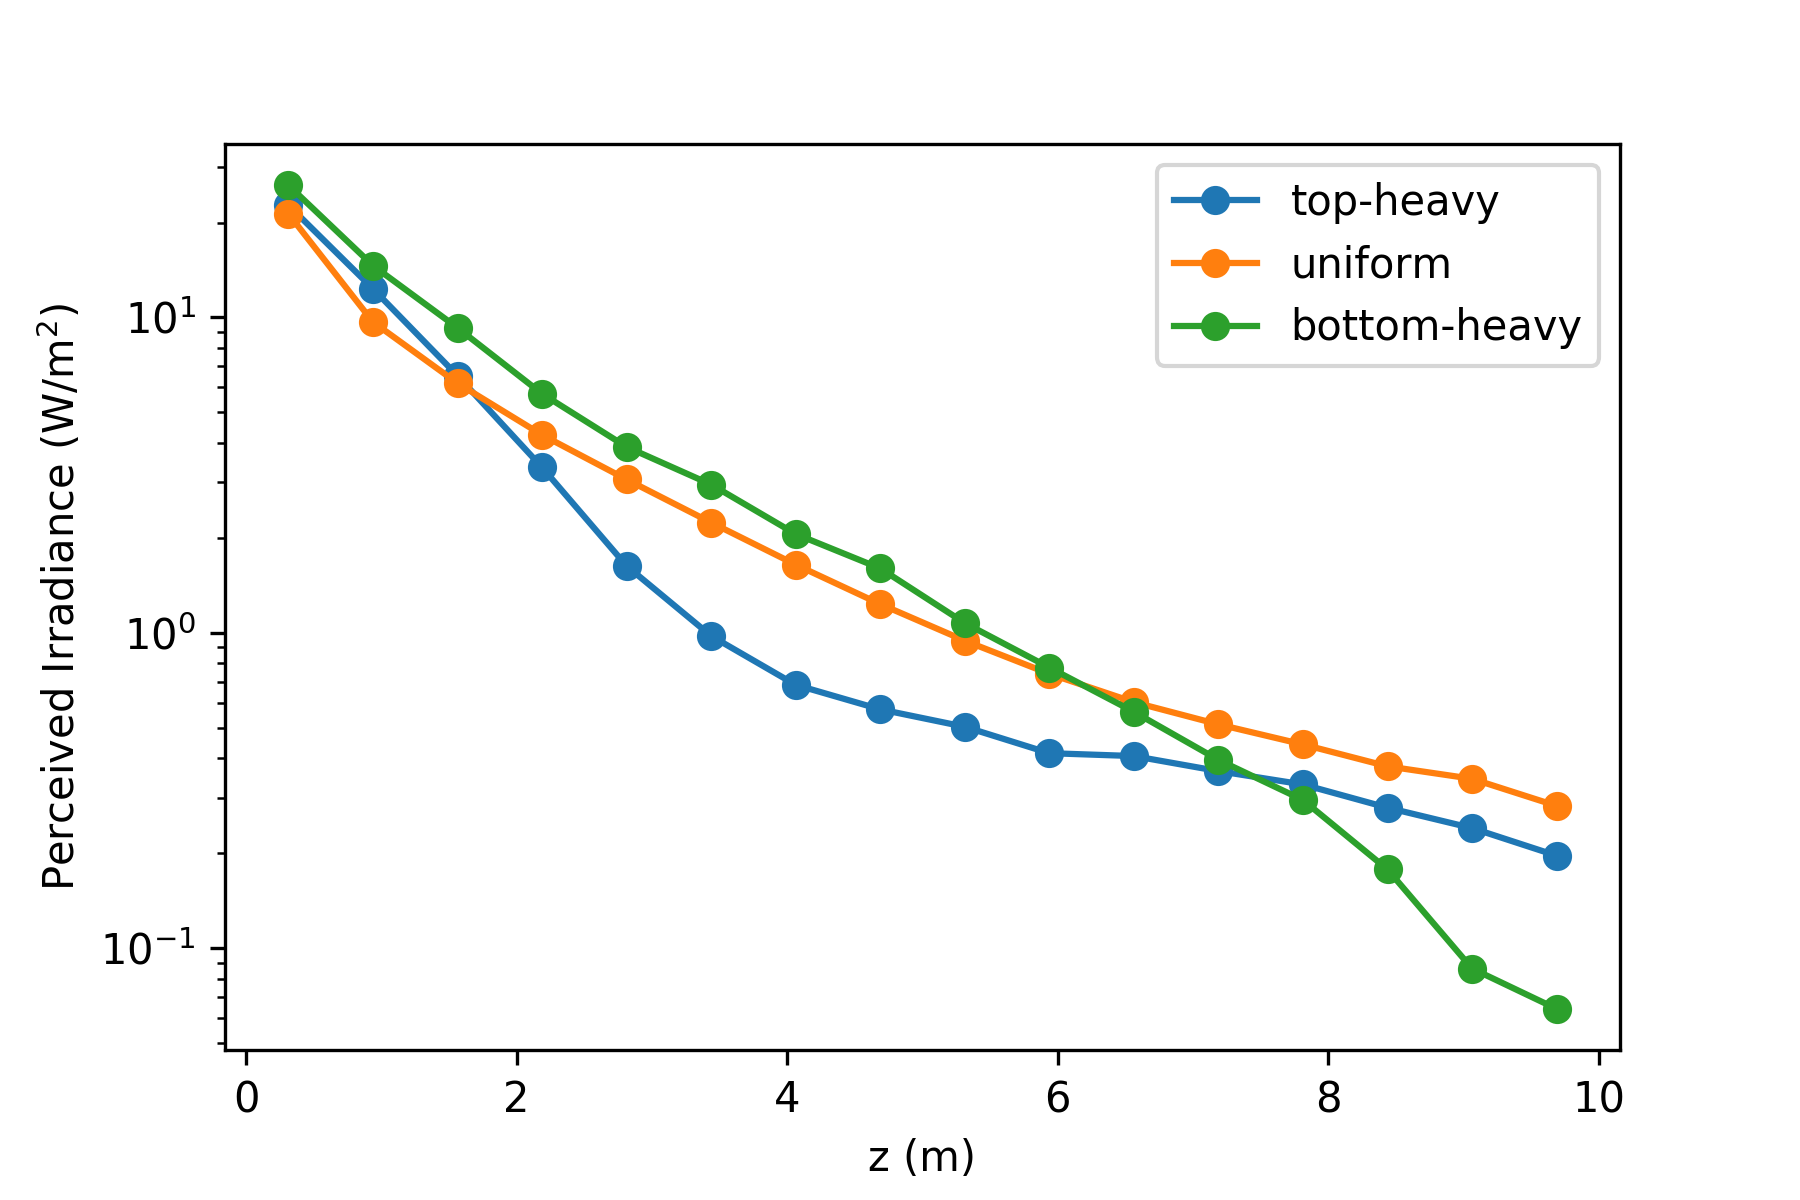
\includegraphics[width=4in]{sens_analysis_kelp_profile}
  \caption{Several kelp profiles}
\end{figure}

\begin{figure}[H]
  \centering
  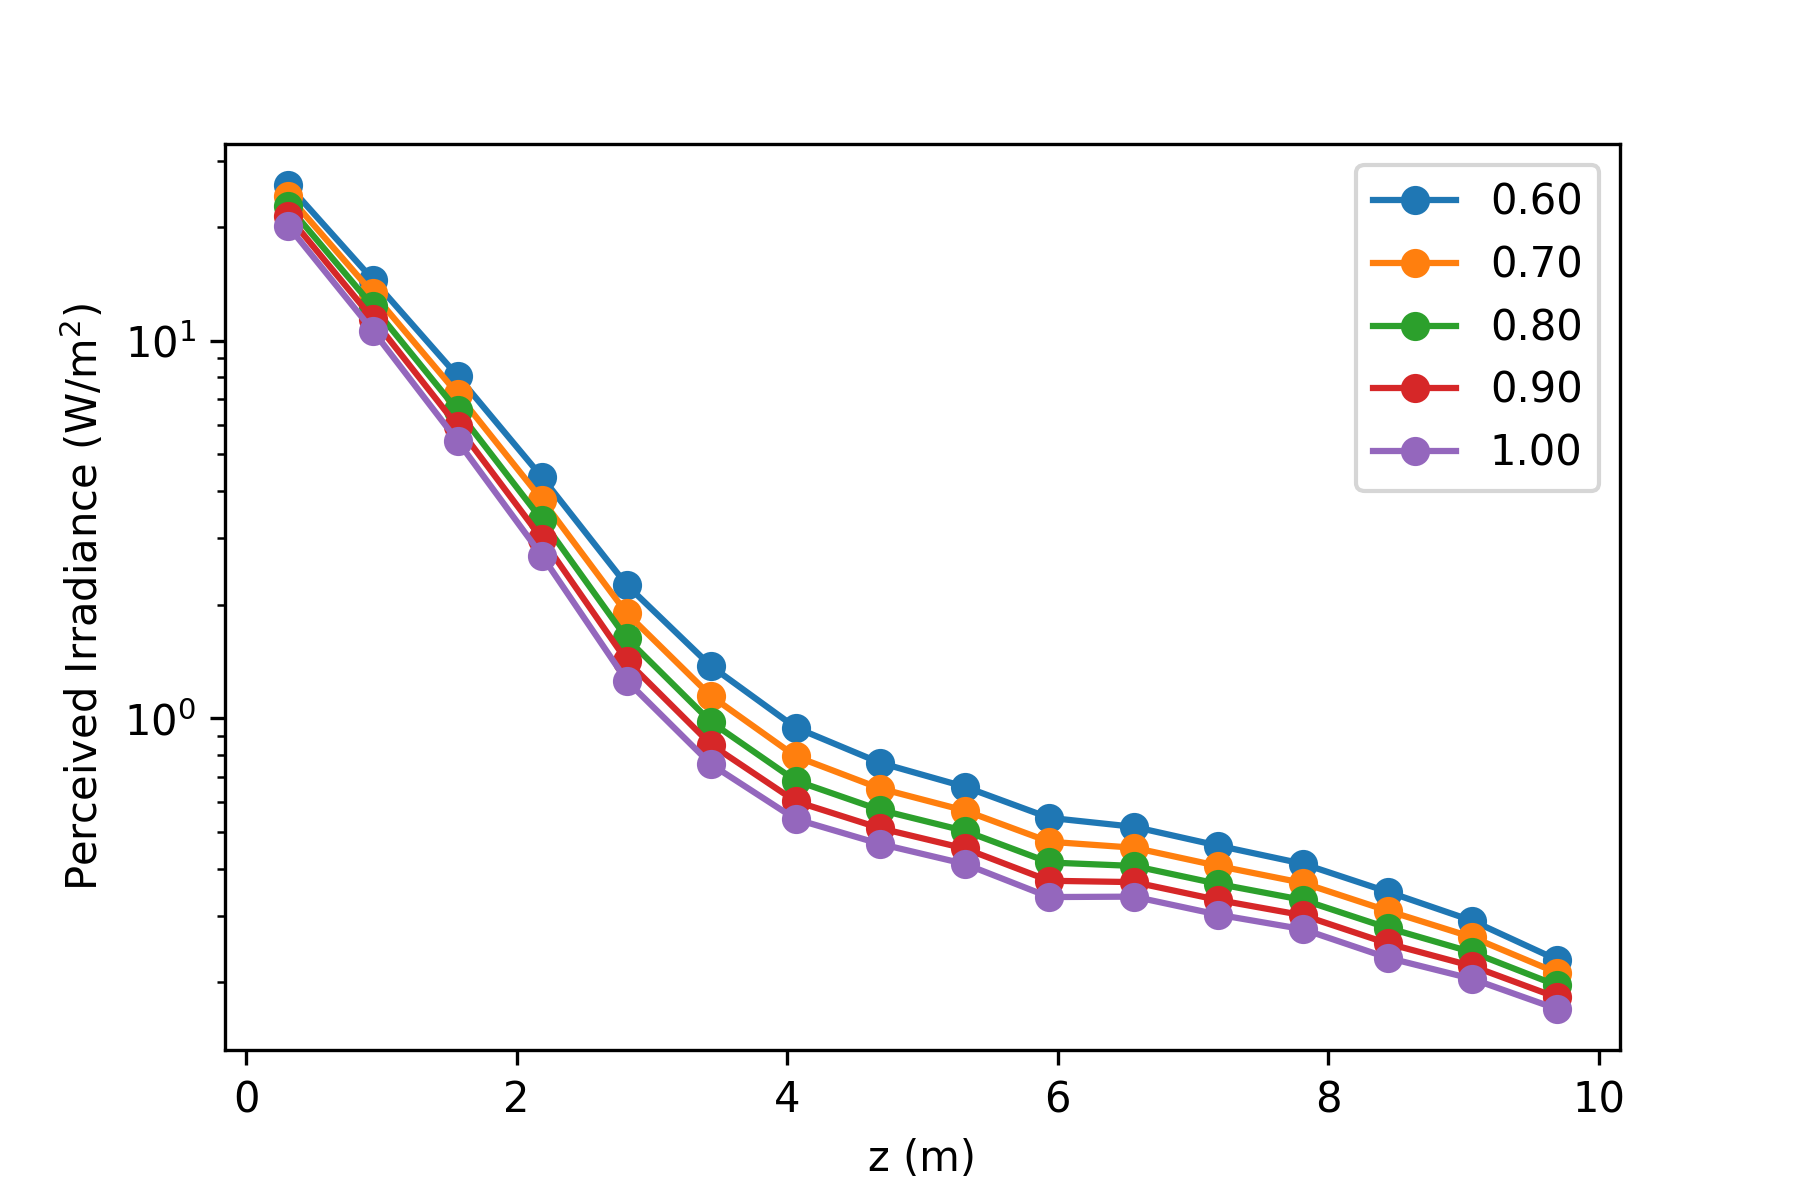
\includegraphics[width=4in]{sens_analysis_absorptance_kelp}
  \caption{Several values of kelp absorptance}
\end{figure}

\begin{figure}[H]
  \centering
  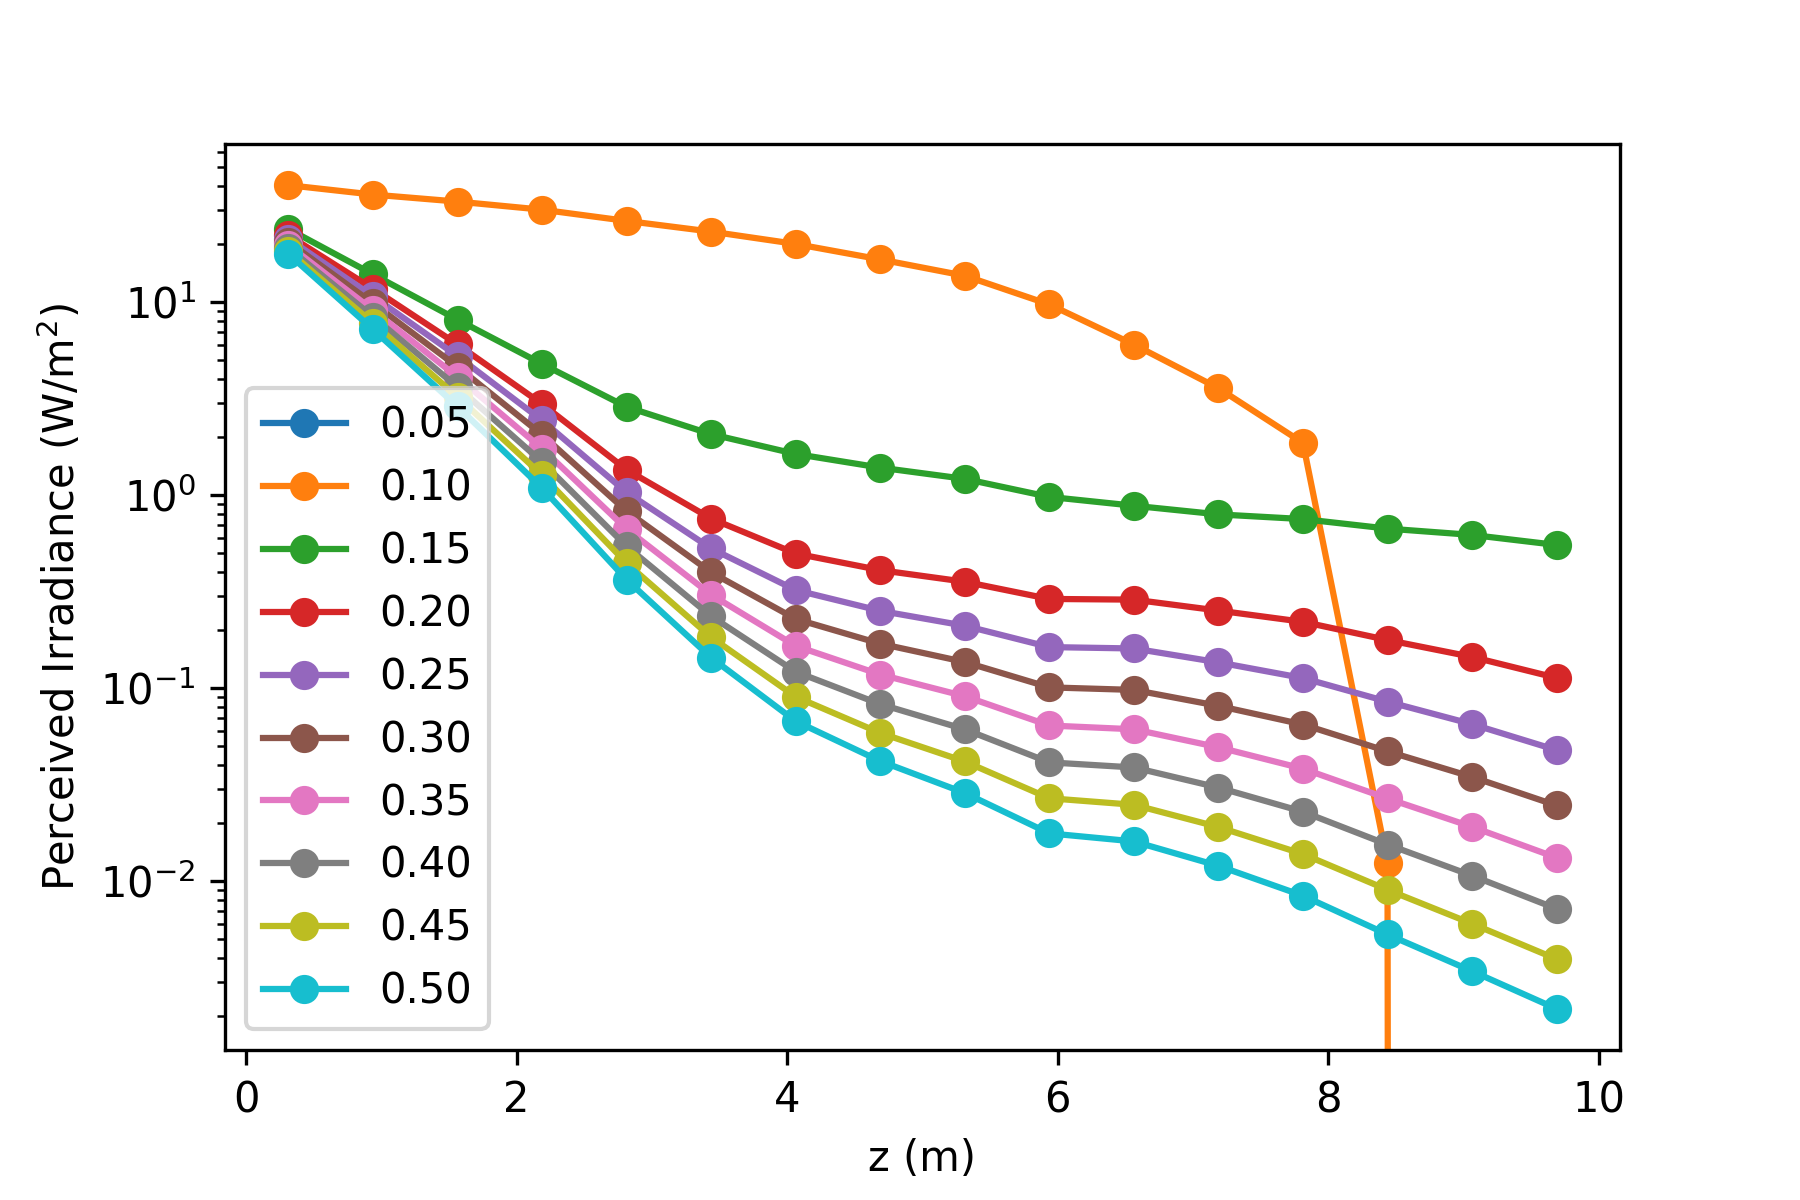
\includegraphics[width=4in]{sens_analysis_a_water}
  \caption{Several values of absorption coefficient of water}
  \label{fig:sens_analysis_a_water}
\end{figure}

\begin{figure}[H]
  \centering
  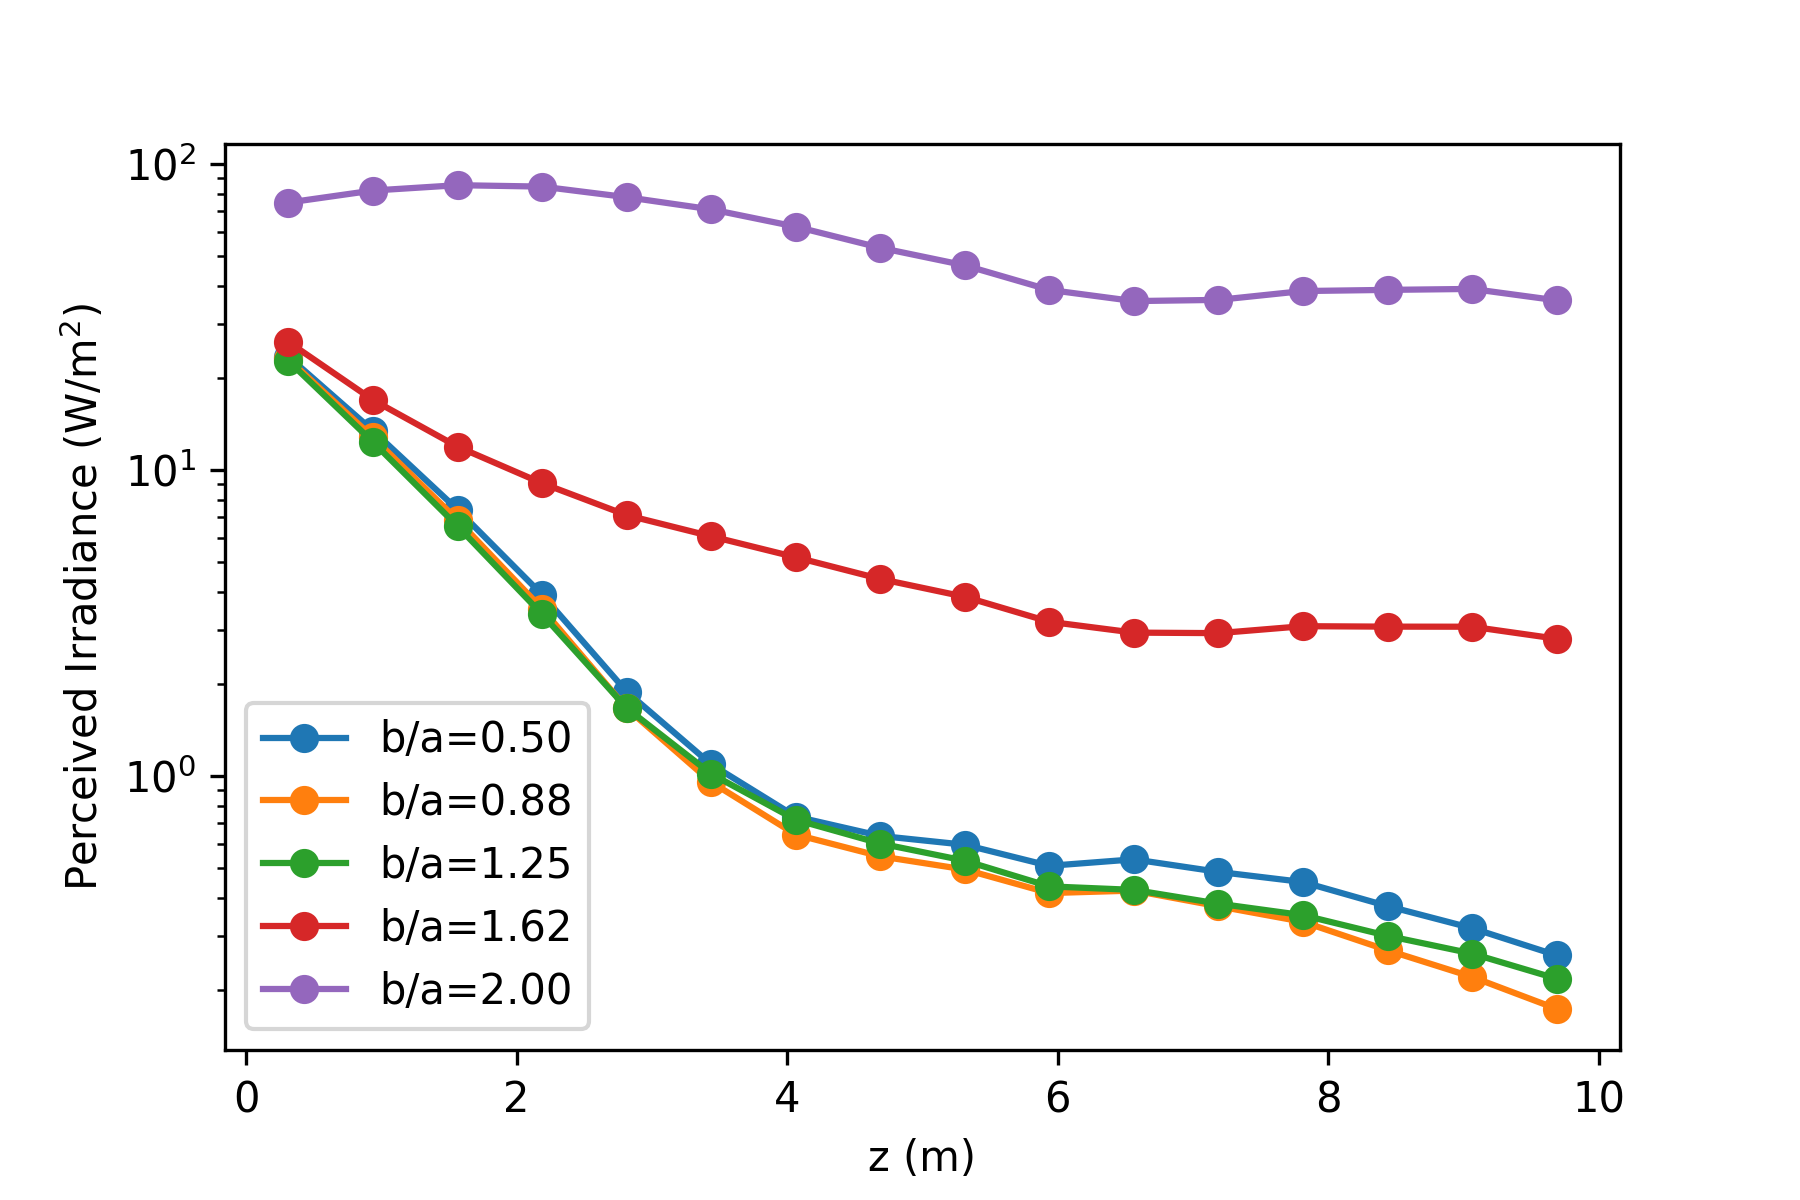
\includegraphics[width=4in]{sens_analysis_b}
  \caption{Several values of scattering coefficient}
  \label{fig:sens_analysis_b}
\end{figure}
 \chapter{CONCLUSION}
\label{chap:conclusion}

We present a probabilistic model for the spatial distribution of kelp, and develop a first-principles model for the light field, considering absorption and scattering due to the water and kelp.
A full finite difference solution is presented, and an asymptotic approximation based on discrete scattering events is subsequently developed.
The asymptotic approximation is shown to converge to the finite difference solution in cases where the absorption coefficient is the same order
of magnitude as the scattering coefficient or larger.
Otherwise, the solution diverges.

Many aspects of the model have room for future improvement.
The most pressing is probably the development of a model for long-lines, which
is more popular in practice than the vertical lines studied here.
Similar techniques can likely be applied, but the details will of course differ.

One major simplification in the calculation of the kelp model
is the assumption that the fronds are perfectly horizontal.
This could be improved in a straightforward way by including some
probability distribution for the angular elevation as a function of current speed,
similar to the study performed in \citep{norvik_design_2017}.
The cost of implementing polar rotation is that depth layers are no longer isolated.
Rather than integrating the two dimensional length-orientation distribution from
Section \ref{sec:dist_2d} to calculate the spatial kelp distribution,
it would be necessary to perform a triple integral which includes the elevation distribution.
Since frond elevation and azimuathal orientation are both related to current velocity,
it would likely be impossible to ignore the remarks at the end of \ref{sec:dist_2d}, and the
assumption of independent distributions would have to be abandoned.

Of course, real fronds are not rotating planar kites, but have a very dynamic geometry.
To consider out-of-plane frond bending would require a totally different approach.
Whether or not any improved description of the seaweed would merit the substantial work is unclear.
 \bibliographystyle{abbrv}
\bibliography{bio}
\appendix{3}
\chapter{GRID DETAILS}
\label{chap:grid_details}

The width of the spatial grid cells in each dimension are
\begin{align*}
  dx &= \frac{x_{\max}-x_{\min}}{n_x}, \\ 
  dy &= \frac{y_{\max}-y_{\min}}{n_y}, \\ 
  dz &= \frac{z_{\max}-z_{\min}}{n_z}.
\end{align*}
Denote the edges as 
\begin{align*}
  x_i^e &= (i-1)dx \mbox{ for } i=1,\ldots,n_x \\
  y_j^e &= (j-1)dy \mbox{ for } j=1,\ldots,n_y \\
  z_k^e &= (k-1)dz \mbox{ for } k=1,\ldots,n_z 
\end{align*}
and the cell centers as
\begin{align*}
  x_i &= (i-1/2)dx \mbox{ for } i=1,\ldots,n_x \\
  y_j &= (j-1/2)dy \mbox{ for } j=1,\ldots,n_y \\
  z_k &= (k-1/2)dz \mbox{ for } k=1,\ldots,n_z
\end{align*}


Note that in this convention, there are the same number of edges and cells,
and edges precede centers.

Now, we define the azimuthal angle such that
\begin{align*}
  \theta_l = (l-1)d\theta.
\end{align*}
For the sake of periodicity, we need
\begin{align*}
  \theta_1 &= 0, \\
  \theta_{n_\theta} &= 2\pi-d\theta,
\end{align*}
which requires
\begin{equation*}
  d\theta = \frac{2\pi}{n_\theta}.
\end{equation*}

For the polar angle, we similarly let
\begin{equation*}
  \phi_m = (m-1)d\phi
\end{equation*}

Since the polar azimuthal is not periodic, we also store the endpoint, so
\begin{align*}
  \phi_1 &= 0, \\
  \phi_{n_\phi} &= \pi.
\end{align*}

This gives us
\begin{align*}
  d\phi &= \frac{\pi}{n_\phi-1}.
\end{align*}

It is also useful to define the edges between angular grid cells as
\begin{alignat}{3}
  \theta_l^e &= (l-1/2) d\theta, &\quad l&=1,\ldots,n_\theta \\
  \phi_m^e &= (m-1/2) d\phi, &\quad m&=1,\ldots,n_\phi-1.
\end{alignat}

Note that while $\theta$ has its final edge following its final center, this is
not the case for $\phi$.

\begin{figure}[h]
  \centering
  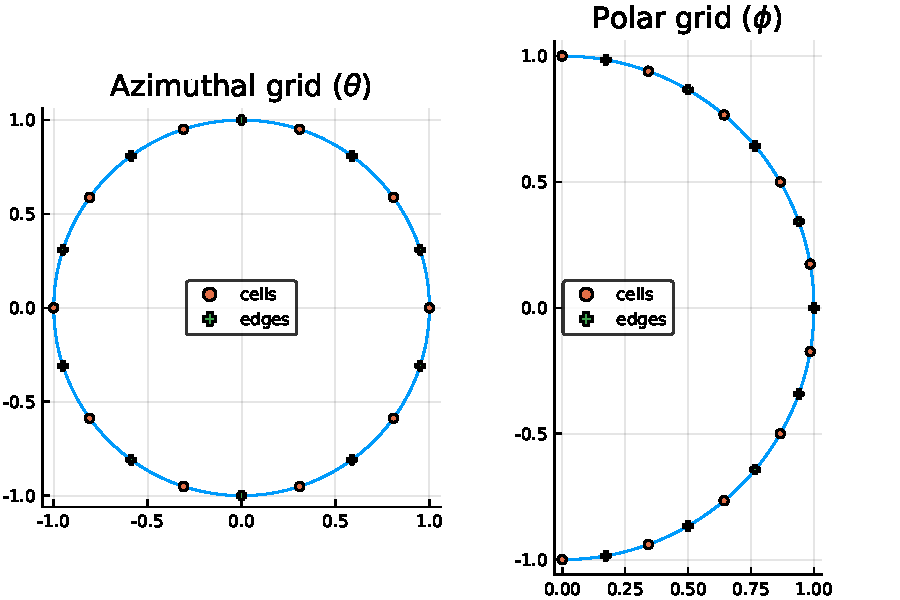
\includegraphics[width=.75\linewidth]{angular_grid_plots}
  \caption{Angular grid}
\end{figure}

The following notation is used.
\begin{align*}
  \hat{l}(p) &= \mbox{mod1}(p, n_\theta) \\
  \hat{m}(p) &= \ceil(p/n_\theta) + 1 \\
  \hat{\theta}_p &= \theta_{\hat{l}(p)} \\
  \hat{\phi}_p &= \phi_{\hat{m}(p)}
\end{align*}

Thus, it follows that
\begin{equation*}
  p = \left( \hat{m}(p)-2\right)n_\theta + \hat{l}(p).
\end{equation*}

Accordingly, define
\begin{equation*}
  \hat{p}(l,m) = (m-1)n_\theta + l.
\end{equation*}

Further, we refer to the angular grid cell centered at $\vec{\omega}_p$ as $\Omega_p$, and the solid angle subtended by $\Omega_p$ is denoted $\abs{\Omega_p}$.
The areas of the grid cells are calculated as follows.
Note that there is a temporary abuse of notation in that the same symbols ($d\theta$ and $d\phi$) are being used for infinitesimal differential and for finite grid spacing.

For the poles, we have
\begin{align*}
  \abs{\Omega_1} = \abs{\Omega_\nomega} &= \int_{\Omega_1} d{\vec{\omega}} \\
  &= \int_0^{2\pi}\int_0^{d\phi/2} \sin\phi\, d\phi\, d\theta \\
  &= 2\pi \cos\phi \Big|_{d\phi/2}^0 \\
  &= 2\pi(1-\cos(d\phi/2))
\end{align*}

And for all other angular grid cells,
\begin{align*}
  \abs{\Omega_p} &= \int_{\Omega_p} d{\vec{\omega}} \\
                 &= \int_{\theta_l^e}^{\theta_{l+1}^e}\int_{\phi_m^e}^{\phi_{m+1}^e} \sin(\phi)\, d\phi\, d\theta \\
                 &= d\theta \int_{\phi_m^e}^{\phi_{m+1}^e} \sin(\phi)\, d\phi \\
                 &= d\theta\left( \cos(\phi_m^e)-\cos(\phi_{m+1}^e) \right).
\end{align*}

 \chapter{RAY TRACING ALGORITHM}
\label{chap:ray_tracing}


In order to evaluate a path integral through the previously described grid, it
is first necessary to construct a one-dimensional piecewise constant integrand
which is discontinuous at unevenly spaced points corresponding to the
intersections between the path and edges in the spatial grid.

Consider a grid center $\vec{p_1} = (p_{1x},p_{1y},p_{1z})$ and a corresponding path $\vec{l}(\vec{x_1}, \vec{\omega}, s)$.
To find the location of discontinuities in the itegrand, we first calculate the
distance from its origin, $\vec{p_0} = \vec{x_0}(\vec{p_1}, \vec{\omega}) = (p_{0x}, p_{0y}, p_{0z})$ to grid edges in each dimension
separately.

Given
\begin{align}
  x_i &= p_{0x} + \frac{s_i^x}{\tilde{s}}(p_{1x}-p_{0x}) \\
  y_j &= p_{0y} + \frac{s_j^y}{\tilde{s}}(p_{1y}-p_{0y}) \\
  z_k &= p_{0z} + \frac{s_k^z}{\tilde{s}}(p_{1z}-p_{0z})
\end{align}

we have
\begin{align}
  s_i^x &= \tilde{s}\frac{x_i-p_{0x}}{p_{1x}-p_{0x}} \\
  s_i^y &= \tilde{s}\frac{y_i-p_{0y}}{p_{1y}-p_{0y}} \\
  s_i^z &= \tilde{s}\frac{z_i-p_{0z}}{p_{1z}-p_{0z}} \\
\end{align}


We also keep a record for each dimension specifying whether the ray increases
or decreases in the dimension. Let
\begin{align}
  \delta_x &= \sign(p_{0x}-p_{1x}) \\
  \delta_y &= \sign(p_{0y}-p_{1y}) \\
  \delta_z &= \sign(p_{0z}-p_{1z})
\end{align}

For convenience, we also store a closely related quantity, $\sigma$ with a value 1 for
increasing rays and 0 for decreasing rays in each dimension
\begin{align}
  \sigma_x = (\delta_x+1)/2 \\
  \sigma_y = (\delta_y+1)/2 \\
  \sigma_z = (\delta_z+1)/2
\end{align}

For this algorithm, we keep two sets of indices. $(i,j,k)$ indexes the grid
cell, and will be used for extracting physical quantities from each cell along
the path.
Meanwhile, $(i^e,j^e,k^e)$ will index the edges between grid cells, beginning
after the first cell. i.e., $i^e=1$ refers not to the plane $x=\xmin$, but to $x=\xmin+dx$.

Let $(i_0, j_0, k_0)$ be the indices of the grid cell containing $\vec{p_0}$.

That is,

\begin{align}
  i_0 &= \ceil\left(\frac{p_{0x}-\xmin}{dx}\right) \\
  j_0 &= \ceil\left(\frac{p_{0y}-\ymin}{dy}\right) \\
  k_0 &= \ceil\left(\frac{p_{0z}-\zmin}{dz}\right)
\end{align}

Then,
\begin{align}
  i_0^e &= i_0 + \sigma_x \\
  j_0^e &= j_0 + \sigma_y \\
  k_0^e &= k_0 + \sigma_z
\end{align}

Now, we calculate the distance from $p_0$ along the path to edges in each dimension.
\begin{align}
  s_i^x = \hat{s}\frac{x_i^e-p_{0x}}{p_{1x}-p_{0x}} \\
  s_j^y = \hat{s}\frac{y_j^e-p_{0y}}{p_{1y}-p_{0y}} \\
  s_k^z = \hat{s}\frac{z_k^e-p_{0z}}{p_{1z}-p_{0z}}
\end{align}

For each grid cell, we check the path lengths required to cross the next $x$, $y$, and
$z$ edge-planes.
Then, we move to the next grid cell in that dimension.
That is,

* We also track $s$, the path length.

Consider $i,j,k$ fixed (denoting the current grid cell).

\begin{align}  
  d = \mbox{argmin}_{x,y,z} \left\{ s_i^x-s, s_j^y-s, s_k^z \right\}
\end{align}

* This doesn't quite make sense yet.
\begin{align}
  \begin{cases}
    i = i+\delta_x, & \mbox{if } d=x \\
    j = j+\delta_y, & \mbox{if } d=y \\
    z = k+\delta_z, & \mbox{if } d=z
  \end{cases}
\end{align}

and

\begin{align}
  \begin{cases}
    i^e = i^e+\delta_x, & \mbox{if } d=x \\
    j^e = j^e+\delta_y, & \mbox{if } d=y \\
    z^e = k^e+\delta_z, & \mbox{if } d=z
  \end{cases}
\end{align}


Then, move to the adjacent grid cell in the dimension which requires the shortest
step to reach an edge. Save $ds$ of the path through this cell. Also save abs.
coef. and source.
 \chapter{FORTRAN CODE}
\label{chap:fortran}

The full FORTRAN implementation of the model described in this thesis.
This code can be found online at:

\begin{verbatim}
https://github.com/OliverEvans96/kelp
https://gitlab.com/OliverEvans96/kelp
\end{verbatim}

utils.f90
\lstinputlisting{utils.f90}

sag.f90
\lstinputlisting{sag.f90}

kelp3d.f90
\lstinputlisting{kelp3d.f90}

rte\_sparse\_matrices.f90
\lstinputlisting{rte_sparse_matrices.f90}

rte3d.f90
\lstinputlisting{rte3d.f90}

kelp\_context.f90
\lstinputlisting{kelp_context.f90}

light\_context.f90
\lstinputlisting{light_context.f90}

asymptotics.f90
\lstinputlisting{asymptotics.f90}

light\_interface.f90
\lstinputlisting{light_interface.f90}

 \end{document}
